\documentclass[12pt]{ucsddissertation}
% mathptmx is a Times Roman look-alike (don't use the times package)
% It isn't clear if Times is required. The OGS manual lists several
% "standard fonts" but never says they need to be used.
%\usepackage{mathptmx}

\usepackage{fontspec}
\usepackage{gfsdidot}          % makes math stuff look neat, but also overrides text stuff
\setmainfont{TeX Gyre Pagella} % forces back text stuff to look neat too
\setmonofont{DejaVuSansMono}   % monospace stuff should look neat too
%\renewcommand{\familydefault}{\sfdefault}
%\usepackage[scaled=1]{helvet}

\usepackage[NoDate]{currvita}
\usepackage{array}
%\usepackage{tabularx}
\usepackage{booktabs}
\usepackage{ragged2e}
\usepackage{microtype}

\usepackage[numbers]{natbib}
%\usepackage[style=ieee,natbib=true]{biblatex}

\usepackage{graphicx}

% Valentin
\usepackage[dvipsnames]{xcolor}
% xcolor must be loaded prior to tikz, pgfplots, showframe, etc.
\let\iint\relax
\let\iiint\relax
\let\iiiint\relax
\let\idotsint\relax

% Removed for preliminary appointment
%\usepackage{showframe}

\usepackage{amsmath} % loaded by mathtools?
\usepackage{amssymb}
\usepackage[english]{babel}
\usepackage{calc}
\usepackage{caption}
\usepackage{color}
\usepackage{cprotect} % to draw a fbox around a minipage, for debugging
\usepackage{DejaVuSansMono}
\usepackage{dsfont}
\let\textlozenge\relax
\usepackage[inline]{enumitem}
\usepackage{environ}
\usepackage{etoolbox}
\usepackage{fontawesome}
\usepackage{forest}
\usepackage{graphicx}
\usepackage{longtable}
\usepackage{ltablex} \keepXColumns % Made me sad for appendix tables, where was it used?
\usepackage{makecell}
\usepackage{mathpartir}
%\usepackage{mathtools} % \coloneqq
\usepackage{mdframed}
\usepackage{minted}
\usepackage{multicol}
\usepackage[parfill]{parskip}
\usepackage{pgfplots}
\usepackage{pifont} % \ding
\usepackage{soul}
\usepackage{syntax}
\usepackage{tabularx}
\usepackage[skins,theorems]{tcolorbox}
\usepackage{tikz}
\usepackage{tikzpeople}
\usepackage{tikz-qtree}
\usepackage{xpatch}
\usepackage[breaklinks=true,pdfborder={0 0 0}]{hyperref}

% gfsdidot makes ∀ and ∃ super ugly, this reverts them to something fine
\DeclareSymbolFont{CMsymbols}{OMS}{cmsy}{b}{n}
\SetSymbolFont{CMsymbols}{bold}{OMS}{cmsy}{ub}{n}
\DeclareMathSymbol{\forall}{\mathord}{CMsymbols}{"38}
\DeclareMathSymbol{\exists}{\mathord}{CMsymbols}{"39}

\definecolor{color01}{HTML}{E6194B}
\definecolor{color02}{HTML}{3CB44B}
\definecolor{color03}{HTML}{FFE119}
\definecolor{color04}{HTML}{4363D8}
\definecolor{color05}{HTML}{F58231}
\definecolor{color06}{HTML}{911EB4}
\definecolor{color07}{HTML}{46F0F0}
\definecolor{color08}{HTML}{F032E6}
\definecolor{color09}{HTML}{BCF60C}
\definecolor{color10}{HTML}{FABEBE}
\definecolor{color11}{HTML}{008080}
\definecolor{color12}{HTML}{E6BEFF}
\definecolor{color13}{HTML}{9A6324}
\definecolor{color14}{HTML}{FFFAC8}
\definecolor{color15}{HTML}{800000}
\definecolor{color16}{HTML}{AAFFC3}
\definecolor{color17}{HTML}{808000}
\definecolor{color18}{HTML}{FFD8B1}
\definecolor{color19}{HTML}{000075}
\definecolor{color20}{HTML}{808080}
\definecolor{color21}{HTML}{FFFFFF}
\definecolor{color22}{HTML}{000000}

\def\mathunderline#1#2{\color{#1}\underline{{\color{black}#2}}\color{black}}

\forestset{
  default preamble={
    for tree={
      align=center,
      draw=black,
      edge={
        ultra thick,
      },
      edge path={
        \noexpand\path[\forestoption{edge}]
        (!u.parent anchor)
        -- +(0,-10pt)
        -| (.child anchor)
        \forestoption{edge label};
      },
      font=\bfseries,
      % inner sep=10pt,
      l sep=30pt,
      % line width=2pt,
      minimum height=20pt,
      minimum width=30pt,
      parent anchor=south,
      rectangle,
      ultra thick,
    }
  }
}

\newcolumntype{Y}{>{\centering\arraybackslash}X}

% defines safecoqinline, a command like coqinline but works in tabular
% environments
\makeatletter
\def\safecoqinline#1{%
\ifx\@footnotetext\TX@trial@ftn
\detokenize{#1}%
\else
\coqinline{#1}%
\fi}
\makeatother

\captionsetup{
  justification=centering,
}

\usetikzlibrary{arrows, calc, fit, positioning, shapes, tikzmark}

\tikzset{
bicolor/.style 2 args={
  dashed,dash pattern=on 4pt off 4pt,#1,
  postaction={draw,dashed,dash pattern=on 4pt off 4pt,#2,dash phase=4pt}
  },
}

\tikzstyle{Matching}=[
black,
dashed,
line width=3pt,
]

\tikzstyle{RoundedDottedPath}=[
densely dotted,
color05,
line width=3pt,
rounded corners=10pt,
]

\tikzstyle{RoundedRectangle}=[
dashed,
draw,
line width=3pt,
rounded corners=10pt,
]

\tikzstyle{NodeLabel}=[
black,
circle,
draw,
fill=white,
font=\bfseries,
inner sep=1pt,
ultra thick,
]

\newtcbox{\bicolorbox}[1][]{
nobeforeafter,math upper,tcbox raise base,
enhanced,frame hidden,boxrule=0pt,
size=fbox,
boxrule=2pt,
colback=white,
%interior style={top color=green!10!white,
%bottom color=green!10!white,middle color=green!50!yellow},
borderline={2pt}{0mm}{color07},
borderline={2pt}{0mm}{color08,dashed},
%fuzzy halo=1pt with green,
#1
}

\graphicspath{ {./images/} }

\AtBeginDocument{%
	\settowidth\cvlabelwidth{\cvlabelfont 0000--0000}%
}

% Fix a mdframed bug where skipbelow is ignored
\makeatletter
\xpatchcmd{\endmdframed}
  {\aftergroup\endmdf@trivlist\color@endgroup}
  {\endmdf@trivlist\color@endgroup\@doendpe}
  {}{}
\makeatother

%\surroundwithmdframed[
%backgroundcolor=white,
%linecolor=white,
%skipabove=1em,
%skipbelow=-0.5em,
%leftmargin=10pt,
%innertopmargin=1pt,
%innerbottommargin=0pt
%]{minted}

\setminted{
  % DO NOT use bgcolor, use mdframed instead
  %bgcolor=white,
  linenos=true,
  style=xcode,
  breaklines=true,
  encoding=utf8,
  fontsize=\small,
  baselinestretch=1,
}

% need bgcolor for the display to be nice in rules
\newmintinline{coq}{bgcolor=white}

% This works for some styles but not all, instead I hijack the tokens directly
% in background.tex

% \AtBeginEnvironment{minted}{%
%   \renewcommand{\fcolorbox}[4][]{#4}}
% \def\dontdofcolorbox{\renewcommand\fcolorbox[4][]{##4}}

% These do not seem to work...
% \xpatchcmd{\coqinline}{\minted@fvset}{\minted@fvset\dontdofcolorbox}{}{}
% \xpatchcmd{\mintinline}{\minted@fvset}{\minted@fvset\dontdofcolorbox}{}{}

\makeatletter
% \AtBeginEnvironment{minted}{\dontdofcolorbox}
% \def\dontdofcolorbox{\renewcommand\fcolorbox[4][]{##4}}
% \xpatchcmd{\inputminted}{\minted@fvset}{\minted@fvset\dontdofcolorbox}{}{}
% \xpatchcmd{\mintinline}{\minted@fvset}{\minted@fvset\dontdofcolorbox}{}{}

% \expandafter\def\csname PYGmonokai@tok@err\endcsname{
%   \def\PYGmonokai@tc##1{\textcolor[rgb]{0.59,0.88,0.31}{##1}}
%   \def\PYGmonokai@bc##1{\setlength{\fboxsep}{0pt}\colorbox[rgb]{0.88,0.00,0.06}{\strut ##1}}
% }
\makeatother

\makeatletter
\pgfdeclareshape{document}{
\inheritsavedanchors[from=rectangle] % this is nearly a rectangle
\inheritanchorborder[from=rectangle]
\inheritanchor[from=rectangle]{center}
\inheritanchor[from=rectangle]{north}
\inheritanchor[from=rectangle]{south}
\inheritanchor[from=rectangle]{west}
\inheritanchor[from=rectangle]{east}
% ... and possibly more
\backgroundpath{% this is new
% store lower right in xa/ya and upper right in xb/yb
\southwest \pgf@xa=\pgf@x \pgf@ya=\pgf@y
\northeast \pgf@xb=\pgf@x \pgf@yb=\pgf@y
% compute corner of ‘‘flipped page’’
\pgf@xc=\pgf@xb \advance\pgf@xc by-10pt % this should be a parameter
\pgf@yc=\pgf@yb \advance\pgf@yc by-10pt
% construct main path
\pgfpathmoveto{\pgfpoint{\pgf@xa}{\pgf@ya}}
\pgfpathlineto{\pgfpoint{\pgf@xa}{\pgf@yb}}
\pgfpathlineto{\pgfpoint{\pgf@xc}{\pgf@yb}}
\pgfpathlineto{\pgfpoint{\pgf@xb}{\pgf@yc}}
\pgfpathlineto{\pgfpoint{\pgf@xb}{\pgf@ya}}
\pgfpathclose
% add little corner
\pgfpathmoveto{\pgfpoint{\pgf@xc}{\pgf@yb}}
\pgfpathlineto{\pgfpoint{\pgf@xc}{\pgf@yc}}
\pgfpathlineto{\pgfpoint{\pgf@xb}{\pgf@yc}}
\pgfpathlineto{\pgfpoint{\pgf@xc}{\pgf@yc}}
}
}
\makeatother

% OGS recommends increasing the margins slightly.
\increasemargins{.1in}

% These are just for testing/examples, delete them
%\usepackage{trace}
%\usepackage{showframe} % This package was just to see page margins
%\usepackage[english]{babel}
%\usepackage{blindtext}
\overfullrule5pt
% ---

% Required information
\title{Front-end tooling for building and maintaining dependently-typed functional programs}
\author{Valentin Robert}
\degree{Computer Science}{Doctor of Philosophy}
% Each member of the committee should be listed as Professor Foo Bar.
% If Professor is not the correct title for one, then titles should be
% omitted entirely.
\chair{Professor Sorin Lerner}
%\cochair{Professor Gamma Delta} % Optional
% Your committee members (other than the chairs) must be in alphabetical order
\committee{Professor William Griswold}
\committee{Professor James Hollan}
\committee{Professor Ranjit Jhala}
\committee{Professor Todd Millstein}
\degreeyear{2018}

%%%%% General-purpose text macros %%%%%
\newcommand{\define}[1]{\emph{#1}}
\newcommand{\mycite}[1]{\citeauthor{#1}~\cite{#1}}

\newcommand{\Language}[1]{\emph{#1}}
\newcommand{\Tool}[1]{\emph{#1}}
\newcommand{\Gallina}{\Language{Gallina}}
\newcommand{\Ltac}{\Language{Ltac}}
\newcommand{\Vernacular}{\Language{Vernacular}}

\newcommand{\Chick}{\Language{Chick}}
\newcommand{\Coq}{\Language{Coq}}
\newcommand{\CoqIDE}{\Tool{CoqIDE}}
\newcommand{\Haskell}{\Language{Haskell}}
\newcommand{\JavaScript}{\Language{JavaScript}}
\newcommand{\OCaml}{\Language{OCaml}}
\newcommand{\PeaCoq}{\Language{PeaCoq}}
\newcommand{\RxJS}{\Language{RxJS}}
\newcommand{\SerAPI}{\Tool{SerAPI}}
\newcommand{\Snap}{\Language{Snap}}
\newcommand{\TypeScript}{\Language{TypeScript}}

\newcommand{\OperatorColor}{purple}
\newcommand{\Operator}[1]{\textcolor{\OperatorColor}{\ #1\ }}
\newcommand{\Entails}{\Operator{\vdash}}
\newcommand{\HasType}{\Operator{:}}

%\newmintinline{coq}{fontsize=\small}
% \newcommand{\coqinline}[1]{%
%   %\colorbox{monokaibg}{%
%   \parbox[c][0.9em]{\widthof{\mycoq{#1}}}{\mycoq{#1}}%
%   %}%
% }

\newcommand{\modified}[1]{\color{Orange}{#1}}
\newcommand{\repaired}[1]{\color{PineGreen}{#1}}

\newcommand{\rulename}[1]{$\LeftTirNameStyle{#1}$}

\newcommand{\RmApp}{Rm-App}
\newcommand{\RmPi}{Rm-Pi}
\newcommand{\InsApp}{Ins-App}

%%%%% Math-mode macros %%%%%

\newcommand{\opcolor}{purple}
\newcommand{\out}[1]{ \boxed{ \textcolor{teal}{#1} } }
\newcommand{\MathPatches}[3]{%
#1 \overset{#2}{\mathbin{\textcolor{\opcolor}{\rightsquigarrow}}} \out{#3}%
}

\newcommand{\App}{\$}
\newcommand{\Mod}{Mod}
\newcommand{\Drop}{Drop}
\newcommand{\Ins}{Ins}
\newcommand{\Keep}{Keep}
\newcommand{\Lam}{\lambda}

\newcommand{\oMod}{\overset{\mathtt{\Mod}}}
\newcommand{\oDrop}{\overset{\mathtt{\Drop}}}
\newcommand{\oIns}{\overset{\mathtt{\Ins}}}
\newcommand{\oKeep}{\overset{\mathtt{\Keep}}}

\newcommand{\Cons}{::}
\newcommand{\permute}[2]{%
\overline{#2}^{\overset{#1}{\rightleftarrows}}%
}
\newcommand{\permuteOp}[2]{%
\overset{\overset{#1}{\rightleftarrows}}{#2}%
}

\newcommand{\mkMathPiRaw}[4]{#3{\Pi} #4{#1} \rightarrow #2}
\newcommand{\mkMathPi}[5]{\mkMathPiRaw{(#2 : #1)}{#3}{#4}{#5}}


\newcommand{\MathCons}[2]{#1 \Cons #2}
\newcommand{\MathDrop}[1]{\oDrop{\Cons} #1}
\newcommand{\MathDropApp}[1]{\oDrop{\App} #1}
\newcommand{\MathDropLam}[1]{\oDrop{\Lam} #1}
\newcommand{\MathDropPi}[1]{\oDrop{\Pi} #1}
\newcommand{\MathHole}{\texttt{\_}}
\newcommand{\MathIns}[2]{#1 \oIns{\Cons} #2}
\newcommand{\MathInsApp}[2]{\mkMathApp{#1}{#2}{\oIns}}
\newcommand{\MathInsAppOp}{\oIns{\App}}
\newcommand{\MathInsLam}[2]{\mkMathLam{#1}{#2}{\oIns}{}}
\newcommand{\MathInsLamOp}{\oIns{\Lam}}
\newcommand{\MathInsPi}[3]{\mkMathPi {#1}{#2}{#3}{\oIns}{}}
\newcommand{\MathInsPiOp}{\oIns{\Pi}}
\newcommand{\MathLam}[2]{\mkMathLam{#1}{#2}{}{}}
\newcommand{\MathLams}[3]{\mkMathLam{#1}{#2}{}{\BarCount{#3}}}
\newcommand{\MathKeepPiOp}{\oKeep{\Pi}}
\newcommand{\MathMod}[2]{#1 \oMod{\Cons} #2}
\newcommand{\MathModAppOp}{\oMod{\App}}
\newcommand{\MathModLamOp}{\oMod{\Lam}}
\newcommand{\MathModPiOp}{\oMod{\Pi}}
\newcommand{\MathPermute}[2]{\permuteOp{#1}{\Cons} #2}
\newcommand{\MathPermuteLams}[2]{\permuteOp{#1}{\lambda} #2}
\newcommand{\MathPermutePis}[2]{\permuteOp{#1}{\Pi} #2}
\newcommand{\MathPi}[3]{\mkMathPi{#1}{#2}{#3}{}{}}
\newcommand{\MathPis}[4]{\mkMathPi{#1}{#2}{#3}{}{\BarCount{#4}}}
\newcommand{\MathReplace}[1]{\mathds{K}({#1})}
\newcommand{\MathSame}{\mathds{1}}

\newcommand{\mkMathApp}[3]{#1 #3{ \$ } #2}

%%% REPAIR %%%

\newcommand{\op}[1]{\textcolor{\opcolor}{#1}}

\newcommand{\boundOp}{\op{\text{Bound}}}
\newcommand{\freshOneOp}{\op{\text{Fresh}_1}}
\newcommand{\freshTwoOp}{\op{\text{Fresh}_2}}
\newcommand{\repairIndOp}{\op{R_{I}}}
\newcommand{\repairProgOp}{\op{R_{P}}}
\newcommand{\repairTermOneOp}{\op{R_{T_1}}}
\newcommand{\repairTermTwoOp}{\op{R_{T_2}}}
\newcommand{\repairTermThreeOp}{\op{R_{T_2}}}
\newcommand{\repairVernacOp}{\op{R_{V}}}
\newcommand{\vernacEnvOp}{\op{E_{V}}}
\newcommand{\repairBranchesOp}{\op{R_{B}}}

\newcommand{\blackbrackets}[1]{\left[ #1 \right]}
\newcommand{\blackdiff}[2]{\blackbrackets{\genfrac{}{}{0pt}{}{#1}{#2}}}
\newcommand{\bound}[1]{\boundOp\op{(}#1\op{)}}
\newcommand{\brackets}[1]{%
  \color{\opcolor} \left[ \normalcolor #1 \color{\opcolor} \right] \normalcolor%
}
\newcommand{\context}[2]{#1 \op{,} #2}
\newcommand{\dcontext}[4]{\context{\diff{#1}{#2}}{\diff{#3}{#4}}}
\newcommand{\denv}[2]{\diff{#1}{#2}}
\newcommand{\diff}[2]{\brackets{\genfrac{}{}{0pt}{}{#1}{#2}}}
\newcommand{\dtau}[1]{\delta_{\tau_{#1}}}
\newcommand{\equals}[2]{#1 \mathbin{\textcolor{\opcolor}{=}} #2}
\newcommand{\freshOne}[3]{\freshOneOp\op{(}\diff{#1}{#2}\op{) =}\ \out{#3}}
\newcommand{\freshTwo}[3]{\freshTwoOp\op{(}#1\op{,}#2\op{) =}\ \out{#3}}
\newcommand{\genericrepair}[3]{\mkrepair{\repairTermTwoOp}{#1}{#2}{#3}{\op{?}}}
\newcommand{\nturnstile}[2]{#1 \mathbin{\textcolor{\opcolor}{\nvdash}} #2}
\newcommand{\qmark}{\textcolor{\opcolor}{?}}
\newcommand{\squiggly}[2]{#1 \mathbin{\textcolor{\opcolor}{\rightsquigarrow}} #2}
\newcommand{\subst}[2]{#1 \leftarrow #2}
\newcommand{\turnstile}[2]{#1\ \mathbin{\textcolor{\opcolor}{\vdash}}\ #2}
\newcommand{\repair}[4]{ \mkrepair{\repairTermOneOp}{#1}{#2}{#3}{#4} }
\newcommand{\repairBranches}[3]{\mksimplerepair{\repairBranchesOp}{#1\op{,}\ #2}{#3}}
\newcommand{\repairInd}[7]{
  \mksimplerepair%
  {\repairIndOp}
  {\diff{#1}{#2}\op{,}\ \diff{#3}{#4}\op{,}\ \diff{#5}{#6}}
  {#7}
}
\newcommand{\repairProg}[3]{
  \repairProgOp\op{(}\blackdiff{#1}{#2}\op{)}\ \op{=}\ \out{#3}
}
\newcommand{\repairTerm}[4]{\mkrepair{\repairTermOneOp}{#1}{#2}{#3}{#4}}
\newcommand{\repairTermWithoutType}[2]{\mksimplerepair{\repairTermThreeOp}{#1}{#2}}
\newcommand{\repairVernac}[3]{
  \repairVernacOp\op{(}\blackdiff{#1}{#2}\op{)}\ \op{=}\ \out{#3}
}

\newcommand{\DefinitionText}{\text{Definition}}
\newcommand{\InductiveText}{\text{Inductive}}
\newcommand{\ConstructorText}{\text{Constructor}}
\newcommand{\GlobalDefinitionText}{\text{GlobalDefinition}}
\newcommand{\GlobalInductiveText}{\text{GlobalInductive}}

\newcommand{\Definition}[4]{ \DefinitionText(\{ #1, #2, #3, #4 \}) }
\newcommand{\Inductive}[5]{ \InductiveText(\{ #1, #2, #3, #4, #5 \}) }
\newcommand{\Constructor}[3]{ \ConstructorText(\{ #1, #2, #3 \}) }
\newcommand{\GlobalDefinition}[3]{ \GlobalDefinitionText(\{ #1, #2, #3 \}) }
\newcommand{\GlobalInductive}[5]{ \GlobalInductiveText(\{ #1, #2, #3, #4, #5 \}) }

\newcommand{\ModifyDefinition}[4]{ \delta_{\DefinitionText}(\{ #1, #2, #3, #4 \}) }
\newcommand{\ModifyInductive}[5]{ \delta_{\InductiveText}(\{ #1, #2, #3, #4, #5 \}) }
\newcommand{\ModifyGlobalDefinition}[3]{ \delta_{\GlobalDefinitionText}(\{ #1, #2, #3 \}) }
\newcommand{\ModifyGlobalInductive}[5]{ \delta_{\GlobalInductiveText}(\{ #1, #2, #3, #4, #5 \}) }

\newcommand{\GlobalDefinitionAnon}{\GlobalDefinitionText(\{ \ldots \})}
\newcommand{\GlobalInductiveAnon}{\GlobalInductiveText(\{ \ldots \})}

\newcommand{\DefinitionAnon}{\DefinitionText(\{ \ldots \})}
\newcommand{\InductiveAnon}{\InductiveText(\{ \ldots \})}

\newcommand{\RepairProg}[1]{R-Prog-#1}

\newcommand{\RProgMod}{\RepairProg{Modify}}
\newcommand{\RProgKeep}{\RepairProg{Keep}}
\newcommand{\RProgSameCons}{\RepairProg{Same-Cons}}

\newcommand{\scalefactor}{1}
\newcommand{\invscalefactor}{1}

\NewEnviron
    {Rules}[2]
    {
      \begin{figure*}
        %\scalebox{\invscalefactor}{
          %\begin{minipage}{\scalefactor\textwidth}
            %\begin{mathpar}
              \BODY
            %\end{mathpar}
          %\end{minipage}
        %}
        \caption{#2}
        \label{#1}
      \end{figure*}
    }

\newcommand{\MathSameProg}{\MathSame_P}
\newcommand{\MathSameVernac}{\MathSame_V}
\newcommand{\MathSameGlobal}{\MathSame_G}

\newcommand{\MathProp}{\mathtt{Prop}}
\newcommand{\MathSet} {\mathtt{Set}}
\newcommand{\MathType}{\mathtt{Type}}

\newcommand{\hasType}[2]{ #1\ \op{:}\ #2 }

\newcommand{\mkrepair}[5]{
  #1
  \op{(}
  \hasType
  { #2 }
  { \diff{ #4 }{ #5 } }
  \op{) =\ }
  \out{ #3 }
}

\newcommand{\MathLocalAssum}[2]{ ( #1 : #2 ) }
\newcommand{\MathLocalDef}[3]{ ( #1 : #2 \coloneqq #3 ) }

\newcommand{\mksimplerepair}[3]{
  #1
  \op{(}
  #2
  \op{) =\ }
  \out{ #3 }
}

\newcommand{\RModPi}{\RepairTerm{Mod-$\Pi$}}
\newcommand{\RInsPi}{\RepairTerm{Ins-$\Pi$}}
\newcommand{\RDropPi}{\RepairTerm{Drop-$\Pi$}}
\newcommand{\RPermutePis}{\RepairTerm{Permute-$\Pi$s}}
\newcommand{\RReplace}{\RepairTerm{Replace}}
\newcommand{\RSame}{\RepairTerm{$\MathSame{}$-Other}}
\newcommand{\RSamePi}{\RepairTerm{$\MathSame{}$-$\Pi$}}

\newcommand{\RepairTermPrefix}{RT1}
\newcommand{\GenericRepairPrefix}{R-Term-2}
\newcommand{\UnknownTypeRepairPrefix}{R-Term-2}

\newcommand{\RepairTerm}[1]{\RepairTermPrefix-#1}
\newcommand{\GenericRepair}[1]{\GenericRepairPrefix-#1}
\newcommand{\UnknownTypeRepair}[1]{\UnknownTypeRepairPrefix-#1}

\newcommand{\mkMathLam}[4]{#3{\lambda} #4{#1} \rightarrow #2}

\newcommand{\MathModApp}[2]{ \mkMathApp{#1}{#2}{\oMod}{} }
\newcommand{\MathModLam}[2]{ \mkMathLam{#1}{#2}{\oMod}{} }
\newcommand{\MathModPi} [3]{ \mkMathPi{#1}{#2}{#3}{\oMod}{} }
\newcommand{\MathKeepPi}[1]{ \MathKeepPiOp \rightarrow #1 }

\newcommand{\MathAnnot}[2]{#1 : #2}

\newcommand{\UTRApp}{\UnknownTypeRepair{App}}
\newcommand{\UTRMatch}{\UnknownTypeRepair{Match}}
\newcommand{\UTRPi}{\UnknownTypeRepair{Pi}}
\newcommand{\UTRType}{\UnknownTypeRepair{Universe}}
\newcommand{\UTRVar}{\UnknownTypeRepair{Var}}
\newcommand{\UTRAnnot}{\UnknownTypeRepair{Annot}}
\newcommand{\UTRHole}{\UnknownTypeRepair{Hole}}
\newcommand{\UTROtherwise}{\UnknownTypeRepair{Otherwise}}

\newcommand{\repairArgsOp}{\op{R_{Fn}}}

\newcommand{\repairArgs}[5]{
  \op{\repairArgsOp(}#1\op{,} #2\op{,} #3\op{,} #4\op{) =}\ \out{#5}
}

\newcommand{\declDiff}[3]{
  \hasType
      { \diff{ #1 }{ \out{#2} } }
      { \diff{ \op{?} }{ \out{#3} } }
}

\newcommand{\MathMatch}[2]{ \text{match}\ #1\ \text{with}\ #2 }

\newcommand{\RuleRProgSameNil}{
  {
    \inferrule*
    [lab=\RepairProg{Same-Nil}]
    {  }
    {\turnstile%
      { \denv{E}{\delta_E} }
      { \repairProg{[]}{\MathSame}{\MathSame} }
    }
  }
}

\newcommand{\RuleRProgModify}{
  {
    \inferrule*
    [lab=\RepairProg{Modify}]
    {
      {\turnstile%
        { \denv{E}{\delta_E} }
        { \repairVernac{v}{\delta_v}{\delta_v'} }
      }
      \and
      {\turnstile%
        { \denv{v \Cons{} E}{\MathMod{\delta_v'}{\delta_E}} }
        { \repairProg{p}{\delta_p}{\delta_p'} }
      }
    }
    {\turnstile%
      { \denv{E}{\delta_E} }
      { \repairProg{\MathCons{v}{p}}{\MathMod{\delta_v}{\delta_p}}{\MathMod{\delta_v'}{\delta_p'}} }
    }
  }
}


\setlength\parindent{0.5in}
%\titleformat\paragraph{\sectioningformatting\normalsize\bfseries}{\theparagraph}{1em}{}

% Start the document
\begin{document}
% Begin with frontmatter and so forth
\frontmatter
\maketitle
\makecopyright
\makesignature
% Optional
% \begin{dedication}
% \setsinglespacing
% \raggedright % It would be better to use \RaggedRight from ragged2e
% \parindent0pt\parskip\baselineskip
% In recognition of reading this manual before beginning to format the
% doctoral dissertation or master's thesis; for following the
% instructions written herein; for consulting with OGS Academic Affairs
% Advisers; and for not relying on other completed manuscripts, this
% manual is dedicated to all graduate students about to complete the
% doctoral dissertation or master's thesis.

% In recognition that this is my one chance to use whichever
% justification, spacing, writing style, text size, and/or textfont that
% I want to while still keeping my headings and margins consistent.
% \end{dedication}
% % Optional
% \begin{epigraph}
% \vskip0pt plus.5fil
% \setsinglespacing
% {\flushright
% True ease in writing comes from art, not chance,\\
% As those move easiest who have learn'd to dance.\\
% 'T is not enough to no harshness gives offence,---\\
% The sound must seem an echo to the sense.

% \vskip\baselineskip
% \textit{Alexander Pope}\par}
% \vfil
% \begin{center}
% You write with ease to show your breeding,\\
% But easy writing's curst hard reading.

% \vskip\baselineskip
% \textit{Richard Brinsley Sheridan}
% \end{center}
% \vfil
% \noindent Writing, at its best, is a lonely life. Organizations for
% writers palliate the writer's loneliness, but I doubt if they improve
% his writing. He grows in public stature as he sheds his loneliness and
% often his work deteriorates. For he does his work alone and if he is a
% good enough writer he must face eternity, or the lack of it, each day.

% \vskip\baselineskip
% \hskip0pt plus1fil\textit{Ernest Hemingway}\hskip0pt plus4fil\null

% \vfil
% \end{epigraph}

% Next comes the table of contents, list of figures, list of tables,
% etc. If you have code listings, you can use \listoflistings (or
% \lstlistoflistings) to have it be produced here as well. Same with
% \listofalgorithms.
\tableofcontents
\listoffigures
\listoftables

% Preface
% \begin{preface}
% \end{preface}

% Your fancy acks here. Keep in mind you need to ack each paper you
% use. See the examples here. In addition, each chapter ack needs to
% be repeated at the end of the relevant chapter.
\begin{acknowledgements}
I would like to thank Professor Sorin Lerner for his support as my advisor and
the chair of my committee.

Committing oneself to more than half a decade to a mentally-challenging,
ill-paying, self-motivated job seems like an awful idea.  Yet, it is the ordeal
that most graduate students choose, with little to no foresight as to where the
journey will lead them.  I would like to dedicate the next paragraphs to all
past, current, and future graduate students.

Throughout my six years as a graduate student, I have only been able to visit my
family for a total of three months, both my grandparents passed away after I was
unable to attend a Christmas with them, nor was I able to attend their
respective funeral.  I have needed to move twice, I have needed to TA seven
quarters, I have developed repetitive stress injuries in both my arms, and I
have loaned over \$10.000 to be able to bring this work to completion.

It was not without its worth though.

I have made a solid group of friends without which the journey would have been
too much to bear.  Zachary Tatlock brought me up to speed and offered me several
great opportunities over the years.  Alexander Bakst has been a great roommate,
and it was always nice going for a bike ride to our local coffee shop for
getting work done.  Neha Chachra was a great neighbour, and helped me work
through a lot of mental issues.  Marcela Mendoza also provided mental support,
and helped me focus on working hard for several years, as well as recovering
from hard work sessions by being a great travel companion.  Sohini Manna was
helpful in yelling at me to get things done.  Many recent new friends have made
the final years of the journey wonderful, with lots of music and enjoyable
hangouts.  Dimitar Bounov accompanied me all the way to the end of the journey,
as well as on many memorable hikes.  In particular, my partner Andrea Frank
provided a wonderful emotional support over the past year, and with her
roommate, John Renner, have provided the hosting without which I would not have
been financially able to complete this journey.

I would like to thank the rest of the UCSD Programming Systems group, who have
provided a great environment for research.  In particular, Eric Seidel has
always been tremendous at listening to my issues and offering the perfect,
appropriate technical pointers to resolve them.  My work would often have been
weeks behind without his help.

I would also like to thank the Gallium team of Inria, and in particular my
former mentor, Xavier Leroy, for his great mentorship and the confidence he
inspired in me.  Gabriel Scherer, Jonathan Protzenko, and Nicolas Pouillard,
among many others, have also been excellent lunch and coffee break companions,
who opened my eyes to many of the great concepts of the programming language
community.  Working with all of them was a daily delight.

Andrew Kennedy, who accepted me as an intern at Microsoft Research, gave me the
opportunity to work on a project where I got to improve my understanding of
\Coq{} at a tremendous speed, and introduced me to a project that I had not
believed possible.

Thanks to all the employees of Galois, Inc., where I gave a presentation of my
work earlier this year that was very well received, and followed by great
feedback.  In particular, David Christiansen pointed me to relevant literature
that made part of the work much easier.  It is an immense pleasure to have been
offered a position to work alongside the people I met that day.

Finally, I must thank my mother for her love and support.  This journey must
have been quite the ordeal for her too, and it was hard to convey the reasons
why I still had so much left to do before I was done.  Yet, she was
understanding, and always came through at the most difficult moments, no
questions asked.  Such care is commendable.

Chapters~\ref{chick} and~\ref{coop}, in part, are currently being prepared for
submission for publication of the material.  The dissertation author was the
primary investigator and author of this material.

% I would like to acknowledge Professor Eta Theta for his support as the
% chair of my committee. Through multiple drafts and many long nights,
% his guidance has proved to be invaluable.

% I would also like to acknowledge the ``Smith Clan'' of lab~28, without
% whom my research would have no doubt taken fives times as long. It is
% their support that helped me in an immeasurable way.

% Chapter 2, in full, is a reprint of the material as it appears in
% Numerical Grid Generational in Computational Fluid Mechanics~2009.
% Smith, Laura; Smith, Jane~D., Pineridge Press,~2009. The dissertation
% author was the primary investigator and author of this paper.

% Chapter 3, in part, has been submitted for publication of the material
% as it may appear in Education Mechanics,~2009, Smith, Laura; Smith,
% Jane~D., Trailor Press,~2009. The dissertation author was the primary
% investigator and author of this paper.

% Chapter 5, in part is currently being prepared for submission for
% publication of the material. Smith, Laura; Smith, Jane~D\@. The
% dissertation author was the primary investigator and author of this
% material.

\end{acknowledgements}

% Stupid vita goes next
\begin{vita}
\noindent
\begin{cv}{}
\begin{cvlist}{}
\item[2012 - 2018] Doctorate of Philosophy, Computer Science, University of California San Diego
\item[2008 - 2012] Diploma of Engineering (Master's degree), ENSEIRB-MATMECA
\item[2006 - 2008] Classe pr\'eparatoire, Lyc\'ee Louis Barthou
\item[2001 - 2006] Baccalaur\'eat, Science specialization, Lyc\'ee Saint-Cricq
% \item[1996] Bachelor of Arts, University of California, Berkeley
% \item[1996--2000] U.S. Marines
% \item[2000--2002] Teaching Assistant, Department of Mechanical
% Engineering\\University of California, San Diego
% \item[2002--2006] Research Assistant, University of California, San
% Diego
% \item[2010] Doctor of Philosophy, University of California, San Diego
\end{cvlist}
\end{cv}

% This puts in the PUBLICATIONS header. Note that it appears inside
% the vita environment. It is optional.
\publications

\noindent Robert, V. and Leroy, X., 2012, December. A formally-verified alias
analysis. In International Conference on Certified Programs and Proofs
(pp. 11-26). Springer, Berlin, Heidelberg.

\noindent Ricketts, D., Robert, V., Jang, D., Tatlock, Z. and Lerner, S., 2014,
June. Automating formal proofs for reactive systems. In ACM SIGPLAN Notices
(Vol. 49, No. 6, pp. 452-462). ACM.

% This puts in the FIELDS OF STUDY. Also inside vita and also
% optional.
% \fieldsofstudy
% \noindent Major Field: Engineering (Specialization or Focused Studies)
% \vskip\baselineskip
% Studies in Applied Mathematics\par
% Professors Alpha Beta and Gamma Delta
% \vskip\baselineskip
% Studies in Mechanices\par
% Professors Epsilon Zeta and Eta Theta
% \vskip\baselineskip
% Studies in Electromagnetism\par
% Professors Iota Kappa and Lambda Mu
\end{vita}

% Put your maximum 350 word abstract here.
\begin{dissertationabstract}

Dependently-typed functional languages are increasingly popular, but due to the
complexity of their type systems, there is still a lot of friction in the user
experience, both for beginners who try to learn the concepts, and expert users
who must write and maintain complex code bases.  We explore ways to alleviate
those burdens by providing novel front-end tooling for this class of languages.

In order to help beginners, we explore new visualizations and automation
techniques, focusing on three pain points we identified in the learning process.
We evaluate, via a longitudinal user study and an A-B study, their effectiveness
in terms of learning to use those languages, enjoyment of the learning process,
and productivity on solving beginner-level exercises.

In order to help experts, we prototype a tool that helps in the refactoring of
programs, partially eliminating the tedium of propagating changes throughout
large code bases.  Our tool is built around a small dependently-typed functional
core language, but it supports extensions to richer languages, with similar or
weaker type systems.  We demonstrate this by extending it to support \OCaml{}, a
widely used, modern functional language without dependent types.

% The Abstract begins here. The abstract is limited to 350 words for a
% doctoral dissertation. It should consist of a short statement of the
% problem, a brief explanation of the methods and procedures employed in
% generating the data, and a condensed summary of the findings of the
% study. The abstract may continue onto a second page if necessary. The
% text of the abstract must be double spaced.
\end{dissertationabstract}

% This is where the main body of your dissertation goes!
\mainmatter

% Optional Introduction
\begin{dissertationintroduction}

This thesis aims to design and evaluate novel tools for assisting users of
functional programming languages and proof assistants.

Over the past couple decades, the concept of \emph{functional programming} has
flourished from an academic object of interest to a trending topic in both
academia and industry.  Concepts that used to be mostly relevant in the context
of functional programming languages, for instance, \emph{anonymous functions},
\emph{currying}, \emph{monads}, or \emph{dependent types}, are percolating into
many functional languages as well as mainstream imperative languages.


% This optional section is barely described in the OGS manual other than
% saying it is optional and that it appears in the table of contents
% between the Abstract and the first chapter.

% No formatting guidelines appear so presumably, it should be formatted
% like an ordinary chapter. It should appear after the
% \verb!\mainmatter! macro because it should start on page~1.
\end{dissertationintroduction}

\chapter{Background}\label{background}

This section provides a brief high-level introduction to basic concepts used in
the rest of the dissertation.

\section{Static typing}
\label{static-typing}

% Define static typing

% Discipline of prescribing valid programs from invalid ones

Programmers typically do not write programs by simply manipulating bits in the
computer's memory: most languages offer abstraction mechanisms that let their
users reason at a higher level.  One such high-level abstraction is the notion
of a \define{data type}.  A programmer will want to manipulate structured data
such as numbers, Boolean values, or compound values made out of different values
organized together in some fashion.  They will then use, and possibly define, a
set of operations to work on values from different data types.  Those operations
might sometimes be entirely oblivious to what data type they are manipulating,
but frequently, they will expect some properties out of their input values, and
provide some properties for their output values.

A \define{type system} is a mechanism that enforces some discipline about the
proper use of values in a program according to a set of typing rules.
\define{Typing rules} usually ascribe a type to every value of a program, and
prescribe the typed contexts within which a value of a given type may be used.
A \define{type} can be anything from a simple classification of values according
to their nature (for instance, distinguishing numbers from functions), to more
semantic rules that may sometimes be defined by the user of the language.  In
this dissertation, we will use the notation \mintinline{coq}{t : τ} to indicate
that a term \coqinline{t} has type \coqinline{τ}.

A \define{static} typing discipline allows the programming environment (be it a
compiler, an interpreter, or any other language tool) to reject programs
\textbf{before they run}.  On the opposite, a \define{dynamic} typing discipline
enforces its typing discipline on-the-fly, as programs execute.  This allows
more programs to execute, as long as their execution path does not encounter a
typing violation.  On the other hand, this provides less safety, as latent
errors in the programs stay unnoticed until an execution path triggers them.  In
this dissertation, we will focus solely on static typing disciplines.

There can be many reasons for wanting to reject a program, whether statically or
dynamically.  The simplest case is a breach of expectation between a value and
the context into which it is passed: this is usually called a \define{type
error}.  For instance, a function declared to expect a number input might not be
allowed to receive a string instead.

Another, less obvious, unfortunate reason for rejecting a syntactically-valid,
semantically valid program, is that the static enforcement of typing rules
cannot, in general, be complete.  For instance, dependent type systems (covered
in Section~\ref{dependent-types}) cannot safely ensure their typing discipline
in the presence of arbitrary recursion.  In order to reject all \define{unsafe}
programs before they are run, they must restrict the programs they allow to some
conservative subsets of all \define{safe} programs.

While the idea of preventing programmers from running syntactically-valid
programs might seem like a nuisance, it provides at least two benefits.  From
the programmer's point of view, a disciplined use of the type system can help
them catch, before their program is run, conditions that would make the program
crash were it to be executed.  These conditions can often be indicated at
locations close to the source of error.  The typing discipline can also provide
information that can be leveraged as documentation, or in order to perform code
analyses and transformations that would be intractable or unsafe without types.

Strong typing disciplines can even benefit the programmer tenfold, by providing
means of tracking security properties~\mycite{volpano1997type}, resource usage
and sharing\mycite{naden2012type}, dimensions of
units-of-measure~\mycite{kennedy1994dimension}, etc.

\section{Dependent types}
\label{dependent-types}

This dissertation will mostly focus on \define{dependent} type systems.  A
\define{dependent} type is a type whose definition depends on a program value.
Non-dependent type systems can only express lightweight relationships between
the input and output of functions, as well as lightweight constraints on what
these inputs and outputs may be.  In a dependent type system, one can express
such types as \textit{the type of functions that take a number and return a
larger number}, or \textit{the type of positive numbers that are less than 256}.
In order to express these, one must be able to mention in the type, either
concrete values like \coqinline{256}, or program values like the input value of
the function.

In order to define functions whose output type depend on the value of their
input, dependent type systems must have a \define{type former} (i.e.\ a
syntactic construct) for \define{dependent functions}~\footnotemark.  In the
literature, the type of functions which accept an input value \coqinline{a} of
type \coqinline{A}, and return an output value of type \coqinline{B(a)} (where
\coqinline{B} is a family of types indexed by values of type \coqinline{A}), is
often written as either:

\footnotetext{ \textit{Dependent functions} are sometimes referred to as
\textit{dependent products} in the literature.  Unfortunately, the similar but
different concept of a \textit{dependent pair} is sometimes referred to as
either a \textit{dependent sum} or, confusingly, a \textit{dependent product}.
Since both views are reasonable, and in order to avoid confusion, we will
strictly adhere to the unambiguous names of \textit{dependent function type} and
\textit{dependent pair type} in this dissertation. }

% Pygments/minted put annoying boxes on Unicode because the Coq lexer is stupid
\makeatletter
\expandafter\def\csname PYGlovelace@tok@err\endcsname{\def\PYGlovelace@bc##1{\textcolor[rgb]{0.0,0.0,0.0}{##1}}}
\makeatother

\begin{itemize}

  \item \coqinline{(a : A) → B(a)} % $(a : A) \rightarrow B(a)$

  \item \coqinline{∀(a : A), B(a)}
  % $\forall (a : A), B(a)$
        ~\footnote{The $\forall$ symbol is pronounced ``for all''.}

  \item \coqinline{Π(a : A) → B(a)} % $\Pi (a : A) \rightarrow B(a)$
        ~\footnote{The $\Pi$ symbol may also be pronounced ``for all'' in such context, or ``pi''.}

\end{itemize}

\noindent
We will tend to use the latter, and refer to those types as $\Pi$-types.

When a dependent function takes several arguments, we will group them all into a
single $\Pi$, and coalesce successive values of the same type in groups under
the same set of parentheses.  In practice, this means that the types:

\noindent
\coqinline{Π(a : X) (b c : Y) (d : Z) → R(a, b, c, d)}

\noindent
and

\noindent
\coqinline{Π(a : X) → Π(b : Y) → Π(c : Y) → Π(d : Z) → R(a, b, c, d)}

\noindent
are syntactically equivalent, and we will favor the former (shorter) syntax.

% Introduce Π-telescopes

Nested $\Pi$-types, that is, ones that appear to the right of the arrow of an
enclosing $\Pi$-type, can depend on the values of the previously quantified
variables.  We call a \define{$\Pi$-telescope} any sequence of $\Pi$-types
\emph{directly} nested within one another.  We can summarize them in a list of
bindings and their types, where each type is allowed to, but does not have to,
depend on previous bindings.  For instance, the type:

\noindent
\coqinline{Π(a : X) (b : Y(a)) (c : Z(a)) → R(a, b, c)}

\noindent
contains a telescope of three bindings (namely, \coqinline{a}, \coqinline{b},
and \coqinline{c}), and the type of the last two bindings depend on the value of
the first binding.

Dependent types may also manifest themselves in other forms depending on the
constructs of the language that integrates them.  For instance, languages with
records may allow dependent records, where the type of some fields may depend on
the value of some other fields.  A typical example is the packing of a plain
data structure with extra properties that we want it to have, for instance,
ensuring the binary-search-tree (or \define{BST}) property of a binary tree:

\begin{minted}{coq}
Inductive BinarySearchTree a := MakeBinarySearchTree
  { tree  : BinaryTree a
  , isBST : IsBinarySearchTree tree
  }.
\end{minted}

For the scope of this dissertation, we do not handle such features explicitly,
but believe that the constructions we present are amenable to the introduction
of those features: the simplest flavor of dependent records can be simulated
using a combination of constructs we cover.

\section{Proof assistants}

Our first contribution focuses mostly on programs built using a \define{proof
assistant}.  A proof assistant is a software tool allowing a user to define
mathematical structures, with their axioms and rules, and carry mechanized
proofs of properties of those structures.  By \define{mechanized}, we mean that
the software has the ability to check that a proof is correct, with respect to a
set of rules.  Many proof assistants rely on the Curry-Howard
isomorphism~\cite{howard1980formulae}, bridging the gap between formal logic and
typed programming.  In those systems, logical propositions can be readily
expressed as types, in the same formal system within which programs can be
defined.  Proofs built this way are essentially programs, whose computational
content is often less interesting than the fact that they are well-typed, and as
such, are \define{witnesses} for the type/proposition they inhabit.

Proof assistants come in a large variety, both from a theoretical point of view,
and in terms of user experience.  On the theory side, there are many logical
systems of interest, and different proof assistants tend to focus on some
classes of those.  For instance, the \Coq{} proof assistant focuses, by default,
on an intuitionistic fragment of the calculus of (co)-inductive constructions,
or \Language{CoC}, but allows itself to be extended with axioms to support
classical reasoning, or extensional notions of equality, if needed.

A proof assistant is typically composed of several interacting pieces:

\begin{itemize}

  \item a \emph{programming language}, allowing the user to define programs that
they wish to execute and/or reason about formally,

  \item a \emph{specification language}, allowing the user to define properties
of programs, or general theorems, that they wish to prove,

  \item a \emph{proof language}, allowing the user to build those proofs.

\end{itemize}

Note that these languages need not be different from one another, and several
languages can help fulfill one of those purposes.  For instance, in the \Coq{}
proof assistant, the programming language and the specification language are the
same language, called \Gallina{}, and the proof language can be either
\Gallina{} itself, or a proof-building scripting language called \Ltac{}.

Learning to use such a proof assistant therefore requires familiarizing oneself
with not only a programming language with a complex type system, but also the
logical foundation of formal proofs, and the idiosyncrasies of the proof
environment of choice.

For the \Coq{} proof assistant, novice users are generally taught to use \Ltac{}
to build proofs, since manually building \Gallina{} terms requires more
expertise and is usually tedious.  An \Ltac{} script is a sequence of commands
(usually called \define{tactics}) directing the proof assistant as to what
logical rules to use in order to progress in building the proof term.  These
tactics include:

\begin{itemize}

  \item \emph{proof-solving tactics}, which attempt to complete a proof
obligation by constructing the complete proof,

  \item \emph{case-splitting tactics}, which break a proof obligation into
several sub-obligations, by using some rule of the formal logic with multiple
antecedents,

  \item \emph{bookkeeping tactics}, which modify the context or the goal of the
current proof obligation, either by adding/removing/reordering/rewriting in
hypotheses, or by performing modifications in the goal.

\end{itemize}

A typical proof can therefore be thought of as a tree, branching on
case-splitting tactics, extending on bookkeeping tactics, and with proof-solving
tactics as leaves.  The proving process is rarely linear: many proofs will
require using concepts such as \emph{case analysis} and \emph{induction} in
order to break down a complex goal into specialized sub-goals that can be solved
separately.  In those sub-cases, one will often need to perform applications and
rewriting using existing theorems.

The \define{application} of a theorem (or a hypothesis) \coqinline{(t : τ)} can
be performed in either a hypothesis or a goal.  To apply it in a hypothesis
\coqinline{(a : α)}:

\begin{itemize}

  \item the type of the applied term, \coqinline{τ}, must reduce to a Π-telescope:

    \coqinline{Π(t1 : τ1) ... (tn : τn) → tr : τr}

  \item the type of the target hypothesis, \coqinline{α}, must be compatible
with of one of the \coqinline{τi} (if there are multiple candidates, the first
such \coqinline{τi} will be considered)

\end{itemize}

It then yields the conclusion of the applied term, \coqinline{τr}, as a
hypothesis, but also adds new obligations for all the other antecedents in the
telescope.  Intuitively, the applied term \coqinline{t} was fully applied, with
formal parameter \coqinline{τi} receiving argument \coqinline{a}, and all other
formal parameters receiving arguments to be determined by solving the new
obligations.  That is, given the context:

\begin{minted}{coq}
A, B, C : Prop
H1 : A → B → C
H2 : B
==================
C
\end{minted}

\noindent applying hypothesis \coqinline{H1} in hypothesis \coqinline{H2} yields
the following two obligations:

\begin{minted}{coq}
(* 1. Hypothesis H2 became the conclusion of H1. *)
A, B, C : Prop
H1 : A → B → C
H2 : C
==================
C
\end{minted}

and:

\begin{minted}{coq}
(* 2. In the original context, one must prove A. *)
A, B, C : Prop
H1 : A → B → C
H2 : B
==================
A
\end{minted}

Conversely, a theorem or hypothesis can be applied to the goal of the current
obligation if its conclusion matches the goal.  It yields an obligation for each
antecedent.  For instance, applying hypothesis \coqinline{H1} from the original
context to the goal would yield the following two obligations:

\begin{minted}{coq}
(* 1. One must prove the first antecedent A. *)
A, B, C : Prop
H1 : A → B → C
H2 : B
==================
A
\end{minted}

and:

\begin{minted}{coq}
(* 2. One must prove the second antecedent B. *)
A, B, C : Prop
H1 : A → B → C
H2 : B
==================
B
\end{minted}

\define{Rewriting} with a theorem or a hypothesis is a similar concept, but for
dealing with equalities (or, more generally, structures that admit equivalence
relations, called \define{setoids}).  We will focus on the simple case of
equalities.  Again, one can either use rewrite in a hypothesis, or over the
goal.  One can rewrite with a theorem or hypothesis as long as its conclusion is
an equality.  The rewriting consists of replacing one side of the equality with
the other side, for a given occurrence.  It is a directed operation, either
replacing the left operand of the binary relation with the right one, or
vice-versa.

For instance, given this original context:

\begin{minted}{coq}
P, Q : ℕ → Prop
x, y, z : ℕ
H1 : Q z → x = y
H2 : P x
==================
P y
\end{minted}

rewriting from left to right with hypothesis \coqinline{H1} in hypothesis
\coqinline{H2} yields the two obligations:

\begin{minted}{coq}
(* 1. x has been replaced with y in H2. *)
P, Q : ℕ → Prop
x, y, z : ℕ
H1 : Q z → x = y
H2 : P y
==================
P y
\end{minted}

and:

\begin{minted}{coq}
(* 2. One must prove the antecedent. *)
P, Q : ℕ → Prop
x, y, z : ℕ
H1 : Q z → x = y
H2 : P x
==================
Q z
\end{minted}

while rewriting from right to left with hypothesis \coqinline{H1} in the goal
yields the two obligations:

\begin{minted}{coq}
(* 1. y has been replaced with x in the goal. *)
P, Q : ℕ → Prop
x, y, z : ℕ
H1 : Q z → x = y
H2 : P x
==================
P x
\end{minted}

and:

\begin{minted}{coq}
(* 2. Again, one must prove the antecedent. *)
P, Q : ℕ → Prop
x, y, z : ℕ
H1 : Q z → x = y
H2 : P x
==================
Q z
\end{minted}

A novice user will need to learn to use these tactics effectively, but will also
need to learn about the families of theorems that are applicable in their proof
development.  For instance, the \Coq{} prelude contains 106 equality theorems,
and importing the module about lists increases this number to 1006.  While there
are facilities to look up theorems of interest based on the shape of their type,
this still lacks in ease of discovery, and it is not rare for one to miss or
re-derive an existing theorem.

\section{Program refactoring}

TODO

\chapter{PeaCoq: novel display and user interaction in proof
assistants}\label{peacoq}

This chapter will focus on the development and evaluation of innovative
front-end features for proof assistants, with a focus on helping novice users.

\section{Background}

A proof assistant is typically composed of several interacting pieces:

\begin{itemize}

  \item a \emph{programming language}, allowing the user to define programs that
they wish to execute and/or reason about formally,

  \item a \emph{specification language}, allowing the user to define properties
of programs, or general theorems, that they wish to prove,

  \item a \emph{proof language}, allowing the user to build those proofs.

\end{itemize}

Note that these languages need not be different from one another, and several
languages can help fulfill one of those purposes.  For instance, in the Coq
proof assistant, the programming language and the specification language are the
same language, called \Gallina{}, and the proof language can be either
\Gallina{} itself, or a proof-building scripting language called \Ltac{}.

Learning to use such a proof assistant therefore requires familiarizing oneself
with not only a programming language with a complex type system, but also the
logical foundation of formal proofs, and the idiosyncrasies of the proof
environment of choice.

For the Coq proof assistant, novice users are generally taught to use \Ltac{} to
build proofs, since manually building \Gallina{} terms requires more expertise
and is usually tedious.  An \Ltac{} script is a sequence of commands (usually
called \define{tactics}) directing the proof assistant as to what logical rules
to use in order to progress in building the proof term.  These tactics include:

\begin{itemize}

  \item \emph{proof-solving tactics}, which attempt to complete a proof
obligation by constructing the complete proof,

  \item \emph{case-splitting tactics}, which break a proof obligation into
several sub-obligations, by using some rule of the formal logic with multiple
antecedents,

  \item \emph{bookkeeping tactics}, which modify the context or the goal of the
current proof obligation, either by adding/removing/reordering/rewriting in
hypotheses, or by performing modifications in the goal.

\end{itemize}

A typical proof can therefore be thought of as a tree, branching on
case-splitting tactics, extending on bookkeeping tactics, and with proof-solving
tactics as leaves.  The proving process is rarely linear: many proofs will
require using concepts such as \emph{case analysis} and \emph{induction} in
order to break down a complex goal into specialized sub-goals that can be solved
separately.  In those sub-cases, one will often need to perform applications and
rewriting using existing theorems.

The \define{application} of a theorem can be performed on either a hypothesis or
a goal.  A theorem or hypothesis can be applied to a hypothesis if the
hypothesis matches one of the antecedents of the theorem.  It then yields the
conclusion of the theorem as a hypothesis, but also adds new obligations for all
the other antecedents. That is, given the context:

\begin{minted}{coq}
A, B, C : Prop
H1 : A → B → C
H2 : B
==================
C
\end{minted}

applying hypothesis \mintinline{coq}{H1} to hypothesis \mintinline{coq}{H2}
yields the following two obligations:

\begin{minted}{coq}
A, B, C : Prop
H1 : A → B → C
H2 : C
==================   (* 1. Hypothesis H2 became the conclusion of H1. *)
C

A, B, C : Prop
H1 : A → B → C
H2 : B
==================   (* 2. In the original context, one must prove A. *)
A
\end{minted}

Conversely, a theorem or hypothesis can be applied to the goal of the current
obligation if its conclusion matches the goal.  It yields an obligation for each
antecedent.  For instance, applying hypothesis \mintinline{coq}{H1} from the
original context to the goal would yield the following two obligations:

\begin{minted}{coq}
A, B, C : Prop
H1 : A → B → C
H2 : B
==================   (* 1. One must prove the first antecedent A. *)
A

A, B, C : Prop
H1 : A → B → C
H2 : B
==================   (* 2. One must prove the second antecedent B. *)
B
\end{minted}

\define{Rewriting} with a theorem or a hypothesis is a similar concept, but for
dealing with equalities (or, more generally, structures that admit equivalence
relations, called \define{setoids}).  We will focus on the simple case of
equalities.  Again, one can either use rewrite in a hypothesis, or over the
goal.  One can rewrite with a theorem or hypothesis as long as its conclusion is
an equality.  The rewriting consists of replacing one side of the equality with
the other side, for a given occurrence.  It is a directed operation, either
replacing the left operand of the binary relation with the right one, or
vice-versa.

For instance, given this original context:

\begin{minted}{coq}
P, Q : nat -> Prop
x, y, z : nat
H1 : Q z → x = y
H2 : P x
==================
P y
\end{minted}

rewriting from left to right with hypothesis \mintinline{coq}{H1} in hypothesis
\mintinline{coq}{H2} yields the two obligations:

\begin{minted}{coq}
P, Q : nat -> Prop
x, y, z : nat
H1 : Q z → x = y
H2 : P y
==================   (* 1. x has been replaced with y in H2. *)
P y

P, Q : nat -> Prop
x, y, z : nat
H1 : Q z → x = y
H2 : P x
==================   (* 2. One must prove the antecedent. *)
Q z
\end{minted}

while rewriting from right to left with hypothesis \mintinline{coq}{H1} in the
goal yields the two obligations:

\begin{minted}{coq}
P, Q : nat -> Prop
x, y, z : nat
H1 : Q z → x = y
H2 : P x
==================   (* 1. y has been replaced with x in the goal. *)
P x

P, Q : nat -> Prop
x, y, z : nat
H1 : Q z → x = y
H2 : P x
==================   (* 2. Again, one must prove the antecedent. *)
Q z
\end{minted}

A novice user will need to learn to use these tactics effectively, but will also
need to learn about the families of theorems that are applicable in their proof
development.  For instance, the Coq prelude contains 106 equality theorems, and
importing the module about lists increases this number to 1006.  While there are
facilities to look up theorems of interest based on the shape of their type,
this still lacks in ease of discovery, and it is not rare for one to miss or
re-derive an existing theorem.

% TODO

These are the three challenges we have identified in the learning process for
novice users:

\begin{enumerate}

  \item conceptualizing and keeping track of the \emph{proof tree structure}
while building proofs,

  \item identifying the effects of a tactic on the proof context,

  \item identifying tactics

\end{enumerate}


\section{Design}

\subsection{Global design of \PeaCoq{}}

We will discuss the global architecture of \PeaCoq{} that allows us to build all
the features we mentioned.  Each feature will then be described individually.

\PeaCoq{} is designed following a client-server architecture.  The server
handles the \Coq{} process, and exposes end-points to communicate with it via
HTTP.\@ The client is a web application, containing the front-end view that users
interact with, and facilities for driving the interactions with the server.  Let
us describe each side further.

\tikzset{>=latex}

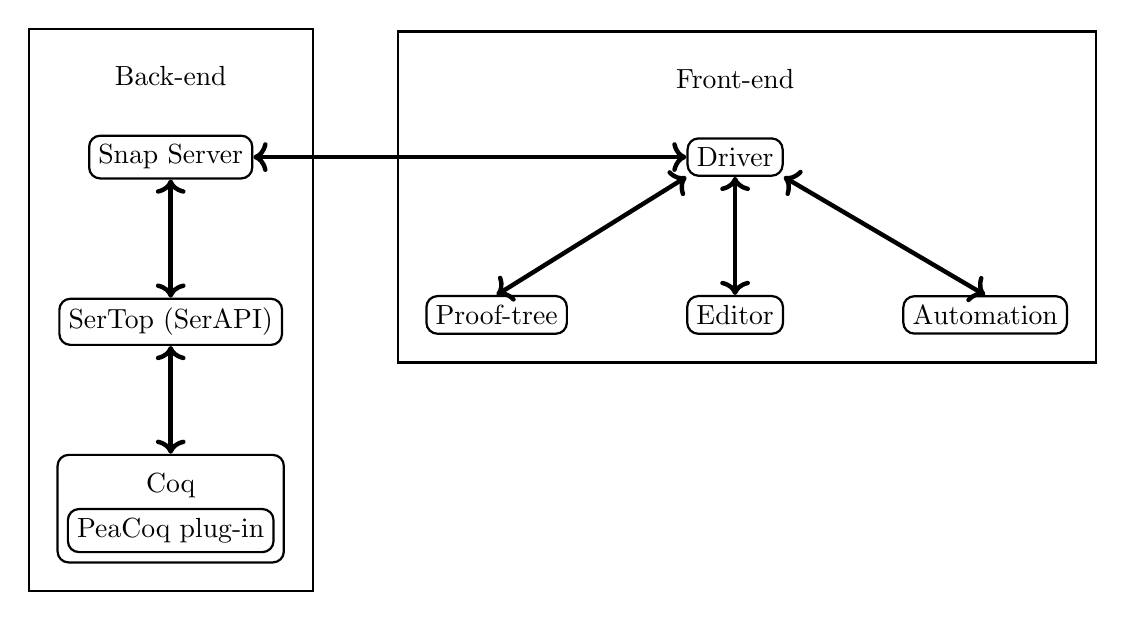
\begin{tikzpicture}[node distance=1.5cm]

  % \tikzstyle{state} = [draw, very thick, fill=white, rectangle, minimum height=3em, minimum width=7em, node distance=8em, font={\sffamily\bfseries}]
  % \tikzstyle{stateEdgePortion} = [black,thick];
  % \tikzstyle{stateEdge} = [stateEdgePortion,->];
  % \tikzstyle{edgeLabel} = [pos=0.5, text centered, font={\sffamily\small}];

  \tikzstyle{outer} = [rectangle,draw = black,thick,inner sep = 10pt];
  \tikzstyle{inner} = [rectangle,rounded corners,draw = black,thick];
  \tikzstyle{arrow} = [thick];

  \node [inner]                         (snap)       {Snap Server};
  \node [inner,below=of snap]           (sapi)       {SerTop (SerAPI)};
  \node [below=of sapi]                 (coq-label)  {Coq};
  \node [inner, below=0cm of coq-label] (plugin)     {PeaCoq plug-in};

  \node [inner,fit={(coq-label) (plugin)}] (coq) {};

  \node [above=0.5cm of snap] (backend-label) {Back-end};
  \node [outer,fit={(backend-label) (snap) (sapi) (coq)}] (backend) {};

  \draw[<->,ultra thick] (snap.south) -- (sapi.north);
  \draw[<->,ultra thick] (sapi.south) -- (coq.north);

  \node [inner,right=5.5cm of snap] (driver)     {Driver};
  \node [inner,below=of driver]     (editor)     {Editor};
  \node [inner,left=of editor]      (prooftree)  {Proof-tree};
  \node [inner,right=of editor]     (automation) {Automation};

  \draw[<->,ultra thick] (driver.south west) -- (prooftree.north);
  \draw[<->,ultra thick] (driver.south) -- (editor.north);
  \draw[<->,ultra thick] (driver.south east) -- (automation.north);

  \node [above=0.5cm of driver] (frontend-label) {Front-end};
  \node [outer,fit={(frontend-label) (driver) (prooftree) (editor) (automation)}] (frontend) {};

  \draw[<->,ultra thick] (snap.east) -- (driver.west);

\end{tikzpicture}

\subsubsection*{Back-end / Server}

In order to let front-ends interact with it, the \Coq{} process exposes an API
that serializes some meta-data and accepts certain commands.  Unfortunately,
prior to \PeaCoq{}'s development, very few tools had used this API, and as a
result, it is lacking both in polish and in features.

The protocol it uses is based upon XML syntax, and exposes commands to
manipulate an abstract document (a collection of \Coq{} sentences) and command
and observe its execution.

While developing \PeaCoq{}, we interacted with Emilio Jesús Gallego Arias, who
was developing a layer over this XML protocol, named \SerAPI{} (for
serialization API).  This layer offers a less rough API based on s-expressions,
abstracting over some minute details of \Coq{}'s implementation.

However, at the time \PeaCoq{} was built, \Coq{} was not exposing enough of its
internals for our needs.  In order to remedy this, we also built a \Coq{}
plug-in to expose this data.  Plug-ins circumvent the IDE API by directly being
compiled and loaded alongside the \Coq{} code: thus, they have access to all the
public interfaces of \Coq{}'s internal modules.  Once our plug-in is loaded, it
registers as a \Vernacular{} command that can be invoked either by users, or
through the IDE API.\@

In order to communicate with front-ends, the back-end is driven by a HTTP
server, based on \Haskell{}'s \Snap{} framework.  The details of its
implementation are fairly mundane: it simply listens to requests from the
front-end, passes them down to \Coq{} through \SerAPI{}, and forwards the
responses back without much processing.  However, this architecture provided
several advantages:

\begin{itemize}

  \item Since the back-end communicates with the front-end over HTTP, the two
need not be on the same physical machine.  For instance, we have had the
back-end running on a powerful Internet-facing machine, and connected it from a
less powerful phone, on public transit.  It worked flawlessly, even in the
presence of computation-intensive loads like our automation, because the
computation was happening server-side.  Meanwhile, the lightweight client was
only processing display and communication with the server.

  \item The back-end was built in such a way that it could accept multiple
connections at once.  Each connection would spawn its own, separate instance of
\Coq{}.  This means that multiple clients could independently connect and work
on the same server.  We used this in our study at the University of Washington,
where one server was shared among all students, who did not need to install
\Coq{} on their machine.

\end{itemize}

\subsubsection*{Front-end / Client}

The front-end of \PeaCoq{} is a simple web application.  It is currently written
in \TypeScript{}, a statically-typed dialect of \JavaScript{}.  We call driver
the part of the code responsible for communicating with the back-end.  We use a
reactive programming library called \RxJS{}, which provides a stream abstraction
for sequences of values.  Messages from the back-end are published as streams,
and each of the components involved in the front-end (namely, the editor, the
proof-tree, and the automation layer) can subscribe to those messages they need
to observe.  Conversely, those components publish streams of commands they'd
like the back-end to process, which the driver subscribes to, and orchestrates
the dispatch of.

This orchestration can require some finesse.  The API provided by \Coq{} is
fairly stateless, that is, \emph{not} in the sense that there are no states, but
rather, in the sense that there is no notion of a current, mutable state.
Instead, each state is given a unique identifier, and subsequent commands may
explicitly state over which previous state they wish to be applied.  This
abstraction holds well at the document level, but unfortunately, some commands
change global, mutable flags, in ways that can be observed.

In other to prevent issues with such observable, mutable state, some sequences
of commands must be processed atomically, that is, no other action may be
interleaved with the sequence.  In order to achieve this, the layers emit their
commands not as a simple sequence of commands, but as a sequence of sequences of
commands, to be dispatched atomically.

This raises another concern: some atomic sequences of commands have data
dependencies.  In particular, later commands often need to know the
\emph{output} of previous commands.  A pervasive example of such a pattern is
found in our automation layer, where commands must be silently tried in the
background, their output must be gathered, and then their effect must be
cancelled.  In order to cancel an action, we must tell \Coq{} the identifier of
the state(s) to be cancelled, but that identifier is only know asynchronously,
in a response from the action that created said state.

Once again, this problem is easily solved by issuing atomic sequences to the
driver not as an array of sequences, but as a stream of commands.  When the
driver chooses to emit a given atomic sequence, it subscribes to it.  It will
subsequently, and asynchronously, receive one or many commands, until the stream
indicates it has completed.  Elements from this stream can be asynchronously
built from other streams, and so we can build those dependent atomic sequences
as:

\begin{minted}{javascript}
// By convention, we put a $ sign behind stream variables.
const commandToCancel = new Add('Command To Cancel')

const answer$ =
  added$.filter(sameTagAs(commandToCancel))
  .takeUntil(completed$.filter(sameTagAs(commandToCancel)))

const output$ = answer$.map(...) // do what you need

const cancelCommand$ =
  answer$.map(a => new Cancel([a.stateId]))

const commands$$ =
  Rx.Observable.concat([
    Rx.Observable.of(commandToCancel),
    cancelCommand$
  ])
\end{minted}

Understanding this code is not necessary, but here is a high-level explanation:

\begin{itemize}

  \item We create (but, do \emph{not} issue yet!) the command whose output we
want to observe.  When a command is created, it acquires a unique tag, that is
sent to \Coq{}, and appears in responses.  This helps us filter those answers
that correspond to this query.

  \item We preemptively subscribe to the stream of answers, looking for ones
with the tag of our command.  In case there is no answer, we also cut this
subscription short when the stream of completed answers emits.  Every command
will produce such an item, so we are guaranteed to terminate.

  \item We can listen to this answer, and compute our output however we see
fit.

  \item We can also listen to this answer in order to emit a cancel command for
it.

  \item The final atomic sequence of commands we send to the driver is the
concatenation of two observables: the command, and its corresponding cancel
command.

\end{itemize}

This is the most important abstraction on the front-end side.  Most of the code
is event-driven by subscribing to those streams and producing streams of
requests.


\subsection{Conceptualizing the proof tree  structure: the tree view}

When a user of the \Coq{} proof assistant writes a proof script using the
\Ltac{} tactic language, they are effectively guiding the tool in building a
derivation, in the underlying formal system, witnessing the truth of the theorem
at hand.

According to the Curry-Howard correspondence, this derivation can be equally
thought of as a well-formed tree, combining axioms and rules of the logical
system, or, as a well-typed λ-term.  For instance, the theorem:

\coqinline{Theorem swap : Π (A B : Prop) → A ∧ B → B ∧ A.}

can be witnessed by the following logical derivation:

\begin{figure*}[htp]

  \scalebox{0.9}{
    \begin{minipage}[t]{\textwidth}

      \begin{mathpar}
        {
          \inferrule*[Right=$\Pi$-intro]
          {
            \inferrule*[Right=$\Pi$-intro]
            {
              \inferrule*[Right=$\Pi$-intro]
              {
                \inferrule*[Right=$\land$-elim]
                {
                  {
                    \inferrule*
                    { }
                    {
                      \ldots , H : A \land B \Entails A \land B
                    }
                  }
                  \and
                  {
                    \inferrule*[Right=$\land$-intro]
                    {
                      {
                        \inferrule*
                        { }
                        {
                          \ldots , H_A : A , H_B : B \Entails A
                        }
                      }
                      \and
                      {
                        \inferrule*
                        { }
                        {
                          \ldots , H_A : A , H_B : B \Entails B
                        }
                      }
                    }
                    {
                      \ldots , H : A \land B , H_A : A , H_B : B \Entails A \land B
                    }
                  }
                }
                {
                  \ldots , H : A \land B \Entails B \land A
                }
              }
              {
                A : \texttt{Prop}, B : \texttt{Prop} \Entails A \land B \rightarrow B \land A
              }
            }
            {
              A : \texttt{Prop} \Entails \Pi (B : \texttt{Prop}) \rightarrow A \land B \rightarrow B \land A
            }
          }
          {
            \Entails \Pi (A\ B : \texttt{Prop}) \rightarrow A \land B \rightarrow B \land A
          }
        }
      \end{mathpar}

    \end{minipage}

  }

\end{figure*}

A corresponding \Coq{} proof following the same strategy matches the structure
of the derivation quite closely:

\begin{minted}{coq}
Proof.
  intros A B H.
  destruct H as [HA HB].
  split.
  + exact HA.
  + exact HB.
Qed.
\end{minted}

and the proof term that it generates also follows the same structure, though it
is less obvious to the beginner:

\begin{minted}{coq}
λ A B H → match H with
          | conj HA HB => conj HB HA
          end
\end{minted}

In fact, the earlier derivation corresponds exactly to the one that the
type-checker follows when checking the type of this last term:

\noindent
\scalebox{0.70}{

  \begin{minipage}{1.3\textwidth}

    \begin{mathpar}
      {
        \inferrule*[Right=$\Pi$-intro]
        {
          \inferrule*[Right=$\Pi$-intro]
          {
            \inferrule*[Right=$\Pi$-intro]
            {
              \inferrule*[Right=$\land$-elim]
              {
                {
                  \inferrule*
                  { }
                  {
                    \ldots , H : A \land B \Entails \coqinline{H} \HasType A \land B
                  }
                }
                \and
                {
                  \inferrule*[Right=$\land$-intro]
                  {
                    {
                      \inferrule*
                      { }
                      {
                        \ldots , H_A : A , H_B : B \Entails \coqinline{HA} \HasType A
                      }
                    }
                    \and
                    {
                      \inferrule*
                      { }
                      {
                        \ldots , H_A : A , H_B : B \Entails \coqinline{HB} \HasType B
                      }
                    }
                  }
                  {
                    \ldots , H : A \land B , H_A : A , H_B : B \Entails \coqinline{conj HB HA} \HasType A \land B
                  }
                }
              }
              {
                \ldots , H : A \land B \Entails \coqinline{match H with conj HA HB => conj HB HA end} \HasType B \land A
              }
            }
            {
              A : \texttt{Prop}, B : \texttt{Prop} \Entails \coqinline{λ H → match ... end} \HasType A \land B \rightarrow B \land A
            }
          }
          {
            A : \texttt{Prop} \Entails \coqinline{λ B H → match ... end} \HasType \Pi (B : \texttt{Prop}) \rightarrow A \land B \rightarrow B \land A
          }
        }
        {
          \Entails \coqinline{λ A B H → match ... end} \HasType \Pi (A\ B : \texttt{Prop}) \rightarrow A \land B \rightarrow B \land A
        }
      }
    \end{mathpar}

  \end{minipage}

}

Therefore, there are two equivalent ways to think about tactics:

\begin{itemize}

  \item they add steps in the derivation tree, possibly finishing, prolonging,
or splitting branches,

  \item equivalently, they add subterms in the partial proof term, possibly
filling, continuing, or adding holes.

\end{itemize}

Unfortunately, due to the sequential nature of the proving process in a proof
assistant, this tree structure is somewhat hidden from the user, who receives
proof obligations one by one in a traversal of the derivation.  For instance, in
the previous proof, after calling \coqinline{split.}, the user is left with two
obligations, originating from the two arguments that the conjunction
introduction rule must receive.  However, in \CoqIDE{}, the main interface to
the proof assistant, the resulting state is displayed thus:

\begin{minted}{coq}
2 subgoals
A, B : Prop
HA : A
HB : B
______________________________________(1/2)
B
______________________________________(2/2)
A
\end{minted}

All remaining sub-obligations are counted, and displayed sequentially, no matter
where they come from.  In this simple example, it is quite easy to follow what
has happened, and to remember that a second sub-obligation must eventually be
solved.  In more complex examples, the delayed sub-obligations can accumulate as
the proof derivation splits into multiple cases, and it is often not immediately
clear where we are in a large proof after we finish a sub-obligation.

The newest versions of \Coq{} include a mechanism to help with this bookkeeping,
named \define{bullets}.  By using bullets like \coqinline{+}, \coqinline{-},
\coqinline{*}, after a splitting point in a proof, the user can indicate their
intent to focus on the sub-obligations generated during that last step.
Preexisting sub-obligations are temporarily hidden, until all newly-generated
sub-obligations are solved, at which point the preexisting ones are restored
back into view.  While this feature gives the user some agency over the list of
proof obligations being displayed at any given time, it still requires the user
to have a mental map of their location in the underlying proof tree.

In order to make this mental map more tangible in the user experience, we
designed a feature that will display this proof tree, as it is being built and
navigated, to the user.

\subsubsection{Building the proof-tree view}

Our proof-tree view is a tree, as shown in Figure~\ref{proof-tree-view-nodes},
whose nodes fall in two categories:

\begin{itemize}

  \item nodes in odd layers are \define{obligation nodes}, that is, they are related to a given proof obligation,

  \item nodes in even layers are \define{tactic nodes}, that is, they are related to the invocation of a given tactic.

\end{itemize}

\begin{figure*}[!htp]
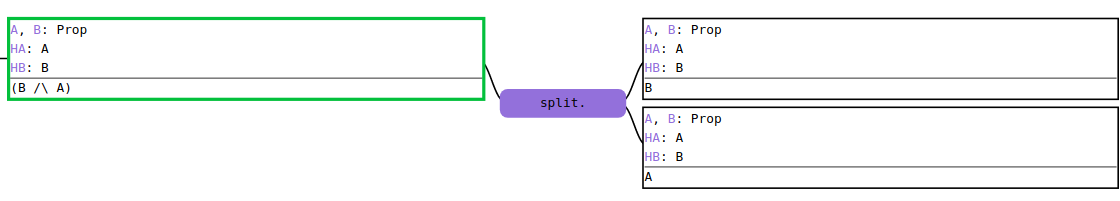
\includegraphics[width=\textwidth]{proof-tree}{\parfillskip=0pt\par}
\caption{Proof-tree view: three obligations nodes and one tactic node}%
\label{proof-tree-view-nodes}
\end{figure*}

When the user enters a proof, a single, root obligation node is created.  This
node corresponds to the current, single proof obligation.  In order to progress,
the user will invoke a tactic.  When they do, a tactic node will be inserted as
a child of the current obligation node, thus denoting that this tactic was ran
from that context.  Depending on the outcome of the tactic execution, one of the
following will happen:

\begin{itemize}

  \item if the tactic yields sub-obligations, these are added as children to the
tactic node, and the focus shifts to the first such sub-obligation,

  \item if the tactic yields no obligation (i.e.\ concludes the current
obligation), then the solved sub-trees are visually folded, and the focus moves
to the next pending obligation, if any.  When there are none, it means the proof
is completed.

\end{itemize}

If the current obligation resulted from the execution of a tactic (i.e. for all
obligations but the root one), the user may backtrack their decision and return
to the state prior to the execution of the parent tactic.


\subsection{Identifying the effects of a tactic: visual diffs}\label{peacoq-design-diffs}

Apart from terminators, which finish an obligation, most tactics will operate a
transformation on the goal of the current context.  The transformations can end
up changing entire types, or replacing sub-terms of some types with other terms.
Some tactics will also add hypotheses, remove some, or reorder hypotheses,
whether voluntarily or as part of how they need to operate.

In order for the user of a proof assistant to assess the usefulness of a
tactic's execution, they must be able to identify what changed by running the
tactic.  This is often done in a ad-hoc way, by going back and forth between the
state before and after the tactic, while visually inspecting differences.  This
is not satisfactory for several reasons.

First, finding out differences using this method is tedious.  Proof contexts
often contain dozens of variables and hypotheses, which makes the task of
finding the changes between two contexts both long, because the user might need
to repeatedly read several lines, and is error-prone, since the user might not
notice a change.

Second, \Coq{} does not offer great facilities for caching results, or viewing
results at a different proof context than the current one.  While rolling back
to the state prior to a tactic's execution is a fairly inexpensive action, due
to the \Coq{}'s state model, going back to the state after the tactic's
execution requires running the tactic again from scratch.  For slow tactics, the
process can be extremely slow, and while the tactic is running, the user might
forget about what they were looking for in the first place.

In order to have a better user experience, one would therefore need to be able
to inspect the state, before and after the execution of a tactic, without having
to run the tactic more than once.  Additionally, visual help indicating which
parts of the context have been modified could help accelerate finding the
effects of a tactic, while reducing the chances of missing a change or
mistakenly spotting a spurious change.

Fortunately, our proof-tree mechanism already provides us with a way of
displaying a before/after view of a proof context with respect to a tactic's
execution.  When a tactic is tried, but not committed to, we can display it as a
child of the current obligation node, and display its result as the child of
this tactic node.  By carefully aligning the two nodes, the user can have an
instant view of the two sides for comparison, without needing to run the tactic
ever again.  We cache those results so that the user can move in the tree
however they want.  Our trees are created in such a way that obligations nodes
have a unique execution history, such that when the user visits the same
obligation node, we can display the same tactic nodes, without needing to run
those tactics again.

We now introduce our notion of \define{visual diffs} as a means to highlight
changes between two proof contexts that are visually juxtaposed.  For a given
hypothesis in the original proof context, one of the following three outcomes
might happen to it as the result of a tactic execution: it may remain the same,
it may disappear, or it may by modified (either by being moved around, of by
having its name, term, or type changed).  Similarly, for a given hypothesis in
the final proof context, it may have originated from an unchanged hypothesis in
the original proof context, from a changed hypothesis in the original proof
context, or it may be a newly introduced hypothesis.

% TODO

\begin{figure*}[!htp]
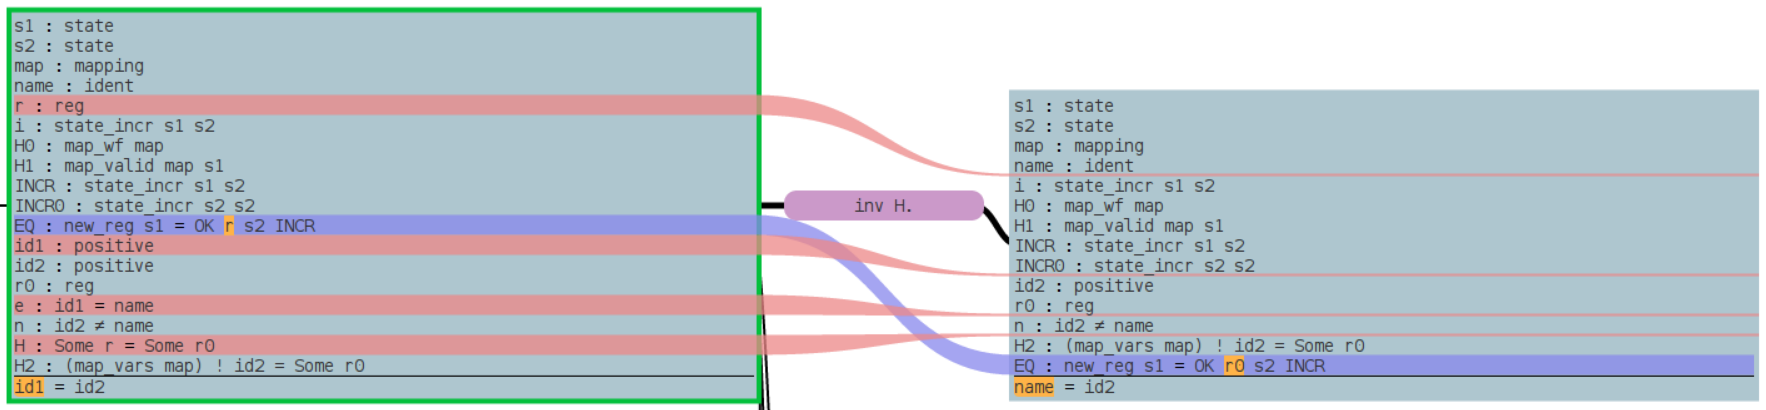
\includegraphics[width=\textwidth]{peacoq-diffs}{\parfillskip=0pt\par}
\caption{Proof-tree visual diff between two obligation nodes}%
\label{proof-tree-diffs}
\end{figure*}


\subsection{Automating tactic exploration in the
background}\label{peacoq-design-automation}

In order to tackle our third identified challenge, that is, helping the user
discover what actions they may take in a given context, we experimented with an
automation technique.  The technique itself is simple: while the user is not
actively entering tactics, we can, in the background, generate and evaluate the
results of a large body of tactics.  We can then estimate which of those tactics
seems relevant to the users and choose how to display them to the user.

The difficulty lies in the details, in particular, we must address the following
problems:

\begin{itemize}

  \item what tactics to try,

  \item which results are relevant,

  \item and how to display those results we deem relevant.

\end{itemize}

We will cover those in order, describing the set of options available.  In our
evaluation, we will highlight which choices we made.

\subsubsection{What tactics to try?}

Because \Coq{} admits \Gallina{} terms as arguments to some \Ltac{} tactics,
there is effectively an infinite number of tactics that can be performed at any
step.  Even ignoring those, many tactics take terms in the environment as
arguments, and the standard library already introduces more than a thousand
terms in the ambient environment.  This makes it clear that an exhaustive search
is not likely.  A couple criteria will help us discern what tactics are worth trying.

First, we can differentiate tactics called \define{terminators} from the ones
that are not.  A terminator is a tactic whose success terminates the current
obligation.  Terminators come in different ways, from very simple ones that find
a proof or a contradiction in the immediate context, to solvers for a given
theory.  For instance, the \coqinline{assumption} tactic is a terminator that
simply looks for an assumption in the current context whose type equates to the
current goal (up to some notion of equality), while the \coqinline{omega} tactic
is a \define{complete} solver for \define{Presburger arithmetic}.  There are
only two outcomes out of the execution of a terminator: either the proof is
found and the tactic succeeds and finishes the current obligation, or its
execution fails.

On the other hand, non-terminator tactics can succeed either by finishing the
current obligation, or by modifying it in any way, or even not doing anything.
They can also lead to the creation of multiple obligations.  For instance, the
\coqinline{split} tactic succeeds on goals that contain a top-level
\define{conjunction}, possibly under a $\Pi$-telescope: it introduces all the
binders in the telescope, and yields two obligations, one for each conjunct.

It is best to test inexpensive terminators first, since a success would mean we
need not look further.  On the other hand, some terminators can effectively
diverge, either by taking an unreasonable amount of time, or by using an
increasingly larger amount of resources, eventually throttling.  In general, we
will need to account for such slowdowns for all tactics with a timeout
mechanism, as we don't want the automation machinery to have a negative
performance impact for our users.

A second important aspect to consider is what arguments to pass to tactics that
require them.  The families of \coqinline{apply} and \coqinline{rewrite}
tactics, for instance, all take as input one term to work with, and, for some, a
second term indicating where to perform the work.  Those terms can either be
variables that are local to the current proof context, or any variable that is
in scope from this file or imported files.  The latter set tends to be between
one and two orders of magnitude larger than the former.  Therefore, while it is
reasonable, but expensive, to try all the proof-local variables, it would be
very expensive to try all identifiers in scope!

\subsubsection{Which results are relevant?}

While we could display all the successful tactics and their outcome to the user,
the amount of information would, in most cases, be overwhelming.  In order for the suggestions to ever be useful, some triage is necessary.

After putting failing tactics out of the picture, one of our first remark is
that many tactics produce the exact same obligations.  Here, one might want to distinguish two close categories:

\begin{itemize}

  \item Two tactics may produce the exact same partial proof term, yielding
equal proof obligations.  This is obviously the case when the two tactics are
aliases of each other, but it can also happen when the two tactics take the same
simple logical step.  Let us refer to those as \define{proof-term equivalent
executions}.

  \item Two tactics may produce the exact same proof obligations (same goals
with same contexts), but build different proof terms.  This could be a concern,
when the terms being built have significant computational differences,
especially in settings where proofs are relevant.  Let us refer to those as
\define{proof-context equivalent executions}.

\end{itemize}

Ideally, we would like to factor out proof-term equivalent executions.  The user
might still care about what tactic is used.  For instance, wherever the
\coqinline{assumption} tactic works, tactics like \coqinline{auto} or
\coqinline{intuition} should also work, but they might do additional work that
is unnecessary.  Similarly, if the assumption being used is called
\coqinline{H}, the tactic \coqinline{exact H} should also work, but it might be
less robust to changes, especially if the name \coqinline{H} was
automatically introduced by \Coq{}.

Finally, the set of tactics available in the \Coq{} proof assistant is not
static: the tactic language is extensible, and users frequently define both
general-purpose and domain-specific tactics.  These can be registered as hints
to the built-in automation mechanism, in which case tactics like
\coqinline{auto} will use them appropriately.  However, as far as we know, at
the current time, there is no built-in mechanism for discovering user-defined
tactics in scope.  An automation mechanism would most likely benefit from such
domain-specific knowledge of tactics to be used in a given proof.

\subsubsection{How to display the relevant results?}

Displaying the outcome of the automation also proves an interesting challenge.
For terminators, or non-terminators that end up solving the current proof
obligation, we can simply indicate to the user that they do.  Tactics that make
progress without solving the proof, however, must be somehow shown to the user
alongside their result.  In the simplest form, one could just present a list of
those tactics, and let the user try them and witness their result on their own.
This imposes quite a bit of cognitive load on the users, as they must visually
inspect one or several proof obligations, trying to understand what changed
between before and after the tactic execution.

To reduce that effort, we benefit from the visualization presented in
Section~\ref{peacoq-design-diffs}.  For each tactic we did not filter out, the
user can align its resulting sub-obligation(s) to the current obligation, and
get visual information about what has changed.

While visual diffs allow the user to quickly inspect the outcome of a given
tactic, if there are too many tactics that make progress, going through them all
one by one can still require a lot of time and concentration.  Some members of
one of our studies indicated the need for grouping the results.  We followed a
static grouping strategy, where tactics were grouped together based on similar
intent: apply tactics, case analysis tactics, rewrite tactics, terminators, etc.
This let users skip over entire classes of tactics that they know are not what
they are currently trying to achieve in the proof.



\section{Evaluation}


\chapter{Chick: a small language and its program repair algorithm}~\label{chick}

This chapter will focus on the development and evaluation of a tool to help
functional programmers propagate changes made to some of their definitions to
the rest of their code.

% \section{Background}

Programs are rarely written once and for all: bugs may be found that must be
fixed, requirements may evolve in ways that require rewriting parts of a
program, and programs may be re-written in semantically-equivalent ways in order
to account for performance, resource-efficiency, or even simply stylistic
concerns.

The concept of \define{refactoring}, which was introduced as early as
in~\citet{wirfs1990surveying}, characterizes program transformations that
preserve the semantics of the program being manipulated.

% TODO FIXME

\begin{figure*}[!htp]

  \noindent%
  \begin{minipage}[t]{0.50\textwidth}
    \begin{minted}[fontsize=\footnotesize,linenos=false]{coq}
Inductive nat : Set :=
| O : nat
| S : ∀ (n : nat), nat.

Inductive list (A : Type)
: Type :=
| nil : list A
| cons : A →
    list A → list A.

Definition a_list
: list nat :=
  cons nat (S O)
    (nil nat).

Definition length :
  ∀ (T : Type),
    list T → nat :=
  λ T l, list_rect T (λ _, nat) O
    (λ _ _ lt, S lt) l.

Fixpoint map :
  ∀ (A B : Type), (A → B) →
    list A →
    list B :=
  λ _ B f l,
    match l with
    | nil _      => nil B
    | cons _ h t =>
      cons B (f h) (map A B f t)
    end.
  \end{minted}
\end{minipage}%
\begin{minipage}[t]{0.50\textwidth}
  \begin{minted}[fontsize=\footnotesize,escapeinside=@@,linenos=false]{coq}
Inductive nat : Set :=
| O : nat
| S : ∀ (n : nat), nat.

Inductive @\modified{vec}@ (A : Type)
: @\modified{nat →}@ Type :=
| @\modified{vnil}@ : vec A @\modified{O}@
| @\modified{vcons}@ : A → @\modified{∀ (n : nat),}@
    @\modified{vec}@ A @\modified{n}@ → vec A @\modified{(S n)}@.

Definition a_list
: @\repaired{vec}@ nat @\repaired{(\_ : nat)}@ :=
  @\repaired{vcons}@ nat @\repaired{(\_ : nat)}@ (S O)
    (nil nat).

Definition length :
  ∀ (T : Type),
    @\repaired{vec}@ T @\repaired{(\_ : nat)}@ → nat :=
  λ T l, @\repaired{vec\_rect}@ T (λ _, nat) O
    (λ _ _ lt, S lt) l.

Fixpoint map :
  ∀ (A B : Type), (A → B) →
    @\repaired{vec}@ A @\repaired{(\_ : nat)}@ →
    @\repaired{vec}@ B @\repaired{(\_ : nat)}@ :=
  λ _ B f l,
    match l with
    | nil _         => nil B
    | @\repaired{vcons}@ _ @\repaired{\_}@ h t =>
      @\repaired{vcons}@ B @\repaired{\_}@ (f h) (map A B f t)
    end.
  \end{minted}
\end{minipage}

\caption{ We demonstrate the propagation of repairs after an inductive
definition is modified.  On the left, the original program.  On the right, we
highlight the user-modified parts in yellow.  The computed repairs are
highlighted in green. }

\label{listtovec}

\end{figure*}


% \section{Design}

We will now describe the syntax of our core language, \Chick{}, that will be the
target of our repair algorithm.  In sections~\ref{chick-design-syntax-terms}
and~\ref{chick-design-syntax-programs}, we will describe the syntax of its
terms, and programs, respectively.

\subsection{Syntax of terms}\label{chick-design-syntax-terms}

\Chick{} is designed as a core functional programming language upon which the
repair algorithm will operate.  The aim was to represent a language such as
\Gallina{}, and as such, \Chick{} is a dependently-typed lambda calculus, with
inductive constructions.  The syntax of \Chick{} is given in this grammar:

\begin{grammar}%
<term> ::= \ %trick LaTeX
\alt <term> : <term>                                           \hfill (type annotation)
\alt <term> <term>                                             \hfill (application)
\alt _                                                         \hfill (hole)
\alt $\lambda$ <binder>, <term>                                \hfill (value abstraction)
\alt match <term> with $\overrightarrow{ \synt{pattern} }$ end \hfill (pattern matching)
\alt $\Pi$(<binder> : <term>) → <term>                         \hfill (type abstraction)
\alt <universe>                                                \hfill (universes)
\alt <var>                                                     \hfill (variable)

<universe> ::= Prop \alt Set \alt Type

<binder> ::= \ % trick LaTeX
\alt <var> \hfill (named)
\alt _     \hfill (anonymous)

<pattern> ::= ($\overrightarrow{ \synt{binder} }$, <term>)
\end{grammar}

The \emph{application}, \emph{value abstraction}, \emph{type abstraction}, and
\emph{variable} constructs, are standard constructs of a dependently-typed
lambda calculus.

The \emph{type annotation} construct lets us ascribe a type to a given term.
The \emph{hole} construct can take the place of a term anywhere: it stands for a
missing value that should be filled by the programmer.  Together, these two
constructs let us have \define{typed holes}, that is, placeholder values whose
type is known.  This proves invaluable throughout the repair algorithm, as we
will see, since there are situations where the algorithm must come up with
arbitrary values, knowing only the type they should bear.  In the absence of
synthesis techniques to generate such values, the algorithm can safely insert a
typed hole, leaving to the programmer the task of figuring out the proper value.

Finally, the \emph{pattern matching} construct is found in languages with
algebraic data types, and lets us dispatch code based on the shape of some
such data type.

We use the same universe names as found in \Gallina{}, though we do not yet
support its cumulative universe hierarchy syntactically.  However, this does
\emph{not} mean that \Chick{} cannot repair \Gallina{} programs that use the
universe hierarchy, but rather, it cannot syntactically represent universe
levels.  Instead, \Chick{} is oblivious to universe levels, so it will repair
programs regardless of their universe level.  The downside is that it cannot
represent explicit universe levels, and as such, might break programs that
require them.  Universe levels can be added almost for free, since the repair
algorithm could simply carry them along and attempt no repair.

While we use the underscore symbol ($\_$) to represent both a hole term and an
anonymous binder, the two concepts can never appear in the same program
location, and therefore, there can be no confusion: in a term context, the
symbol represents a hole, while in a binding context, it represents an anonymous
binder.


\subsection{Syntax of programs}\label{chick-design-syntax-programs}

Our programs are defined as sequences of commands in the following vernacular
(to borrow Coq's parlance):

\begin{grammar}
<program> ::= $\overrightarrow{ \synt{vernac} }$

<vernac> ::= \ %trick LaTeX
\alt Definition(\{ kind : <definition-kind> , name : <var>, type : <term>, body : <term> \})
\alt Inductive(<inductive>)

<definition-kind> ::= Definition | Fixpoint
\end{grammar}

Our \define{definition kinds} follow \Coq{}'s \Vernacular{} conventions: a
\mintinline{coq}{Definition} is \emph{never} recursive, while a
\mintinline{coq}{Fixpoint} is \emph{allowed} to be recursive.  Declarations are
ordered, and may only depend on previous declarations.  This will ease the task
of our repair algorithm, since dependencies are syntactically ordered.  In a
language where declarations are allowed to depend on other declarations backward
\emph{and} forward, we would want to repair programs according to the dependency
tree rather than the syntactic order of declarations.

Inductive definitions are not mutual, and follow the following syntax:

\noindent
\begin{grammar}
<inductive> ::= Inductive(\{\\
name : \synt{var},\\
parameters : $\overrightarrow{ ( \synt{var} , \synt{term} ) }$,\\
indices : $\overrightarrow{ ( \synt{binder} , \synt{term} ) }$,\\
universe : \synt{universe},\\
constructors : $\overrightarrow{ \synt{constructor} }$\\
\})

<constructor> ::= Constructor(\{\\
name : \synt{var},\\
parameters : $\overrightarrow{ ( \synt{binder}, \synt{term} ) }$,\\
indices : $\overrightarrow{ \synt{term} }$\\
\})
\end{grammar}
\vspace{\baselineskip}


\subsection{Describing program modifications with diffed data structures}\label{chick-design-diffs}

We define a family of data types that allows us to capture changes made to
programs from the language presented in
section~\ref{chick-design-syntax-programs}.  We will refer to these descriptions
of changes as \textit{diffs}.  We will usually denote a \textit{diff type}
$\delta_{\tau}$ if it corresponds to values of the diffed type $\tau$.  For
instance, the type $\delta_{\text{universe}}$ would capture how values of type
\coqinline{universe} may have been modified).

Importantly, note that we are not talking about values and types as they appear
in the user's program, but rather, about the internal values and types of the
meta-language.  For instance, if a user changes a \coqinline{bool} value in
their program from \coqinline{true} to \coqinline{false}, we will capture this
change using $\delta_{\text{term}}$, the diff type for $\synt{term}$; whereas
values of the diff type $\delta_{\text{bool}}$ would describe changes made to
boolean flags in the meta-language.

When the user makes a change to their program, we will attempt to guess the
structure of their changes, as a value of one of the program diff type
$\delta_{\text{program}}$.  To illustrate the kind of changes we are interested
in describing, let us go back to our motivating example in
Figure~\ref{listtovec}, where we can observe the following user-provided
modifications (dashed blue outline):

\begin{enumerate}

\item they renamed \coqinline{list} into \coqinline{vec},

\item added an index of type \coqinline{nat},

\item renamed constructor \coqinline{nil} into \coqinline{vnil},

\item instantiated the index for the first constructor with \coqinline{O},

\item renamed constructor \coqinline{cons} into \coqinline{vcons},

\item added a parameter \coqinline{n} of type \coqinline{nat} to the second
  constructor,

\item updated the recursive occurrence's name,

\item updated the recursive occurrence's index,

\item and instantiated the index for the second constructor with \coqinline{(S n)}.

\end{enumerate}

Intuitively, we want to capture changes like insertion, modifications,
deletions, and permutations, at all syntactic levels of the meta-language
(within terms, within inductive declarations).  We will use the same
descriptions to capture user-provided and repair-generated modifications.

Every diff type is accompanied by a patching function, which, given an element
of the diffed type and an element of the diff type produces, when successful, a
patched element.  This operation is partial for many diff types, because they
often capture modifications that only make sense for certain constructors of the
diffed type: for instance, a diff that says the head of a list has been modified
does not apply to the empty list.  We will overload the notation
$\MathPatches{x}{\delta_x}{x'}$ to indicate that $x'$ is the (optional) value
obtained when (successfully) patching $x$ according to the diff $\delta_x$,
using the relevant patching function for that diff type.  In all of our
notations, we use a black frame and a teal highlight to indicate that a value is
an output.

\subsection{Atomic diff}

There are many data types for which we will only capture changes at an atomic
granularity: either the value is the same in the new program, or it has been
replaced with a different, unrelated value.  For instance, a binder can either
have the same name, or have been renamed.  Similarly, the only possible change
to the recursive flag of a definition is to be atomically changed to a different
value.  The parameterized $\delta_{atomic}$ diff type captures such cases for a
given type $\tau$:

\begin{grammar}
<$\delta_{atomic}\ \tau$> ::= \ %trick LaTeX
\alt $\MathSame$                        \hfill (unchanged)
% \alt $\MathReplace{\langle\tau\rangle}$ \hfill (replaced)
\end{grammar}
%
with the following semantics:

\begin{mathpar}

  {
    \inferrule*
    [right=Identity]
    {  }
    {\MathPatches{x}{\MathSame}{x}}
  }

  {
    \inferrule*
    [right=Replace]
    {  }
    {\MathPatches{x}{\MathReplace{y}}{y}}
  }

\end{mathpar}

\subsection{List diff} \label{list-diff}

For lists, we provide a rich selection of diff operations.  The aim is not to
have a canonical representation, but rather to capture closely the intent of
the user modifications:

\begin{grammar}
<$\delta_{\text{list}} \ \tau \ \delta_{\tau}$> ::= \ %trick LaTeX
\alt \synt{$\delta_{\text{atomic}}\ \tau$} \hfill (atomic modification)
\alt \begin{tabular}{p{0.3cm} >{\centering}p{0.6cm} l}$\langle\tau\rangle$
       & $\MathIns{}{}$
       & \synt{$\delta_{list}\ \tau\ \delta_{\tau}$} \\\end{tabular} \hfill
     (insert a head)
\alt \begin{tabular}{p{0.3cm} >{\centering}p{0.6cm} l}$\langle\delta_\tau\rangle$
       & $\MathMod{}{}$
       & \synt{$\delta_{list}\ \tau\ \delta_{\tau}$} \\\end{tabular}
     \hfill (modify and keep the head)
%\alt \begin{tabular}{p{0.3cm} >{\centering}p{0.6cm} l}\quad & $\MathKeep{}$
%       & \synt{$\delta_{list}\ \tau\ \delta_{\tau}$} \\\end{tabular}
%     \hfill (keep the head)
\alt \begin{tabular}{p{0.3cm} >{\centering}p{0.6cm} l}\quad
       & $\MathDrop{}$
       & \synt{$\delta_{list}\ \tau\ \delta_{\tau}$} \\\end{tabular}
     \hfill (drop the head)
\alt \begin{tabular}{p{0.3cm} >{\centering}p{0.6cm} l}\quad
       & FIXME % $\MathPermute{p}{}$
       & \synt{$\delta_{\text{list}}\ \tau\ \delta_{\tau}$} \\\end{tabular}
     \hfill (permute according to a permutation $p$)
\end{grammar}
%
with the following semantics:

\begin{mathpar}
  {
    \inferrule*
    [right=Insert]
    {\MathPatches{l}{\delta_{l}}{l'}}
    {\MathPatches{l}{\MathIns{h}{\delta_{l}}}{(h :: l')}}
  }

  {
    \inferrule*
    [right=Modify]
    {\MathPatches{h}{\delta_{h}}{h'} \quad \MathPatches{t}{\delta_{t}}{t'}}
    {\MathPatches{(h :: t)}{\MathMod{\delta_{h}}{\delta_{t}}}{(h' :: t')}}
  }
\\
  % {
  %   \inferrule*
  %   [right=Keep]
  %   {\MathPatches{t}{\delta_{t}}{t'}}
  %   {\MathPatches{(h :: t)}{\MathKeep{\delta_{t}}}{(h :: t')}}
  % }
  {
    \inferrule*
    [right=Drop]
    {\MathPatches{t}{\delta_{t}}{t'}}
    {\MathPatches{(h :: t)}{\MathDrop{\delta_{t}}}{t'}}
  }

  {
    \inferrule*
    [right=Permute]
    {\MathPatches{(h_{p(1)} \Cons \ldots \Cons h_{p(|p|)} \Cons t)}{\delta}{l}}
    {\MathPatches{(h_1 \Cons \ldots \Cons h_{|p|} \Cons t)}{\MathPermute{p}{\delta}}{l}}
  }

\end{mathpar}

Note that we defined the semantics of $\MathModPiOp$ so that it both modifies
and keeps the head: the recursive occurrence in rule~\rulename{Modify},
$\delta_t$, therefore applies to the tail $t$ and not the whole list after the
head has been repaired.  On the other hand, the recursive occurrence in
rule~\rulename{Permute}, $\delta$, targets the entire list after the permutation
is performed, not solely the tail: this is necessary because we will want to
perform modifications of elements after having shuffled them around.

\subsection{Term diff}

The diffs for terms include atomic changes, as well as insertion, modification,
deletion, and permutation of most constructors.  We illustrate a couple of
these:

\begin{grammar}
<$\delta_{term}$> ::= \ %trick LaTeX
\alt \synt{$\delta_{atomic}\ t$} \hfill (atomic modification)
\alt \synt{$\delta_{term}$} $\oIns{ \$ }$ \synt{$\delta_{term}$} \hfill
(insert application)
\alt $\oIns{\lambda}$ \synt{v}, \synt{$\delta_{term}$} \hfill (insert value
abstraction)
\alt $\oIns{\Pi}$ (\synt{v} : \synt{$\delta_{term}$}),
\synt{$\delta_{term}$} \hfill (insert type abstraction)
\alt ... \hfill (other insertions)
\alt ... \hfill (removals/modifications/permutations)
\end{grammar}

\noindent Note that we use an infix dollar sign ($\$$) as a symbol for function
application in our diffs, even though we use an infix space for function
application in our terms, which is not ideal but should prevent confusion.  For
our purpose, we biased the diffs on binary operations in the least surprising
way: deleting an application keeps its left child, i.e. removes the function
call and keeps the function (see \rulename{\RmApp}), while deleting a
\coqinline{Pi} keeps its right child, i.e. removes the value being quantified
but keeps the return type (see \rulename{\RmPi}).  For insertion, we allow
maximal flexibility by passing the entire old term to all recursive occurrences:
for instance, the diff $(\MathInsApp{\MathSame}{\MathSame})$ turns any term $t$
into the self-application $(t\ t)$ (see \rulename{\InsApp}).  However, it is
often the case that only one recursive occurrence will use the original term,
while the other ones will replace it: for instance, the diff
$(\MathInsApp{\MathSame}{\MathReplace{x}})$ turns any term $t$ into the
application $(t\ x)$.

\begin{mathpar}
  {
    \inferrule*
    [right=\RmApp]
    {\MathPatches{f}{\delta}{f'}}
    {\MathPatches{f\ x}{\MathDropApp{\delta}}{f'}}
  }

  {
    \inferrule*
    [right=\RmPi]
    {\MathPatches{\tau_{2}}{\delta}{\tau_{2}'}}
    {\MathPatches{\MathPi{\tau_{1}}{x}{\tau_{2}}}{\MathDropPi{\delta}}{\tau_{2}'}}
  }

  {
    \inferrule*
    [right=\InsApp]
    {\MathPatches{t}{\delta_1}{t_1} \quad \MathPatches{t}{\delta_2}{t_2}}
    {\MathPatches{t}{\MathInsApp{\delta_1}{\delta_2}}{t_1\ t_2}}
  }

\end{mathpar}

\subsection{Other diff types}

We also need diffs for many other internal data types.  Diff types for tuples
are derived from diff types of their constituents in a straightforward way.
Inductive data type definitions, as well as constructor definitions, behave
essentially like a tuple of all their arguments, so their diff type is derived
accordingly.


\section{Repairing programs by propagating changes} \label{chick-design-repair}

In this section, we assume that we are given an original program $p$, that is, a
sequence of vernacular commands as described in
Section~\ref{chick-design-syntax-programs}, and a diff of that program
$\delta_p$ as described in Section~\ref{chick-design-diffs}, capturing a partial
refactoring made by the user.  We assume that the original proof script
type-checked, and attempt to build a repaired diff $\delta_p'$ such that:

\begin{itemize}

\item $\delta_p'$ contains the changes from $\delta_p$,

\item $\delta_p'$ completes the refactoring started by $\delta_p$, by
propagating forward the changes from $\delta_p$ to use-sites that must be
repaired to account for those changes,

\end{itemize}
%
where propagating changes forward means:

\begin{itemize}

\item propagating renaming of constants and variables,

\item propagating changes in the number, order, and type of arguments to
functions, obtained from their definition, to their use-site,

\item propagating changes in the definition of inductive data types to use-sites
of the type, its constructors, and its eliminators (those will be explained in
more details in section~\ref{deriving}).

\end{itemize}

We give a top-down description of the repair algorithm, starting at the level of
whole programs, descending all the way to terms and data type definitions.

\input{chick-design-repair-program}

\input{chick-design-repair-vernacular}

\input{chick-design-repair-term}



% \documentclass[preview]{standalone}

\usepackage{fontspec}
\usepackage{gfsdidot}          % makes math stuff look neat, but also overrides text stuff
\setmainfont{TeX Gyre Pagella} % forces back text stuff to look neat too
\setmonofont{DejaVuSansMono}   % monospace stuff should look neat too

\usepackage[dvipsnames]{xcolor} % must be loaded prior to tikz, pgfplots, etc.
\let\iint\relax
\let\iiint\relax
\let\iiiint\relax
\let\idotsint\relax
\usepackage{amsmath} % loaded by mathtools?
\usepackage{amssymb}
\usepackage[english]{babel}
\usepackage{booktabs}
\usepackage{calc}
\usepackage{caption}
\usepackage{color}
\usepackage{DejaVuSansMono}
\usepackage{dsfont}
\let\textlozenge\relax
\usepackage[inline]{enumitem}
\usepackage{environ}
\usepackage{etoolbox}
\usepackage{fontawesome}
\usepackage{forest}
\usepackage{graphicx}
\usepackage{longtable}
\usepackage{ltablex} \keepXColumns % Made me sad for appendix tables, where was it used?
\usepackage{makecell}
\usepackage{mathpartir}
%\usepackage{mathtools} % \coloneqq
\usepackage{mdframed}
\usepackage{minted}
\usepackage{multicol}
\usepackage[parfill]{parskip}
\usepackage{pgfplots}
\usepackage{pifont} % \ding
\usepackage{soul}
\usepackage{syntax}
\usepackage{tabularx}
\usepackage[skins,theorems]{tcolorbox}
\usepackage{tikz}
\usepackage{tikzpeople}
\usepackage{tikz-qtree}
\usepackage{xpatch}
\usepackage[breaklinks=true,pdfborder={0 0 0}]{hyperref}

% gfsdidot makes ∀ and ∃ super ugly, this reverts them to something fine
\DeclareSymbolFont{CMsymbols}{OMS}{cmsy}{b}{n}
\SetSymbolFont{CMsymbols}{bold}{OMS}{cmsy}{ub}{n}
\DeclareMathSymbol{\forall}{\mathord}{CMsymbols}{"38}
\DeclareMathSymbol{\exists}{\mathord}{CMsymbols}{"39}

\definecolor{monokaibg}{HTML}{272822}
\definecolor{color01}{HTML}{E6194B}
\definecolor{color02}{HTML}{3CB44B}
\definecolor{color03}{HTML}{FFE119}
\definecolor{color04}{HTML}{4363D8}
\definecolor{color05}{HTML}{F58231}
\definecolor{color06}{HTML}{911EB4}
\definecolor{color07}{HTML}{46F0F0}
\definecolor{color08}{HTML}{F032E6}
\definecolor{color09}{HTML}{BCF60C}
\definecolor{color10}{HTML}{FABEBE}
\definecolor{color11}{HTML}{008080}
\definecolor{color12}{HTML}{E6BEFF}
\definecolor{color13}{HTML}{9A6324}
\definecolor{color14}{HTML}{FFFAC8}
\definecolor{color15}{HTML}{800000}
\definecolor{color16}{HTML}{AAFFC3}
\definecolor{color17}{HTML}{808000}
\definecolor{color18}{HTML}{FFD8B1}
\definecolor{color19}{HTML}{000075}
\definecolor{color20}{HTML}{808080}
\definecolor{color21}{HTML}{FFFFFF}
\definecolor{color22}{HTML}{000000}

\def\mathunderline#1#2{\color{#1}\underline{{\color{black}#2}}\color{black}}

\forestset{
  default preamble={
    for tree={
      align=center,
      draw=black,
      edge={
        ultra thick,
      },
      edge path={
        \noexpand\path[\forestoption{edge}]
        (!u.parent anchor)
        -- +(0,-10pt)
        -| (.child anchor)
        \forestoption{edge label};
      },
      font=\bfseries,
      % inner sep=10pt,
      l sep=30pt,
      % line width=2pt,
      minimum height=20pt,
      minimum width=30pt,
      parent anchor=south,
      rectangle,
      ultra thick,
    }
  }
}

\newcolumntype{Y}{>{\centering\arraybackslash}X}

% defines safecoqinline, a command like coqinline but works in tabular
% environments
\makeatletter
\def\safecoqinline#1{%
\ifx\@footnotetext\TX@trial@ftn
\detokenize{#1}%
\else
\coqinline{#1}%
\fi}
\makeatother

\captionsetup{
  justification=centering,
}

\usetikzlibrary{arrows, calc, fit, positioning, shapes, tikzmark}

\tikzset{
bicolor/.style 2 args={
  dashed,dash pattern=on 4pt off 4pt,#1,
  postaction={draw,dashed,dash pattern=on 4pt off 4pt,#2,dash phase=4pt}
  },
}

\tikzstyle{Matching}=[
black,
dashed,
line width=3pt,
]

\tikzstyle{RoundedDottedPath}=[
densely dotted,
color05,
line width=3pt,
rounded corners=10pt,
]

\tikzstyle{RoundedRectangle}=[
dashed,
draw,
line width=3pt,
rounded corners=10pt,
]

\tikzstyle{NodeLabel}=[
black,
circle,
draw,
fill=white,
font=\bfseries,
inner sep=1pt,
ultra thick,
]

\graphicspath{ {./images/} }

% Fix a mdframed bug where skipbelow is ignored
% \makeatletter
% \xpatchcmd{\endmdframed}
%   {\aftergroup\endmdf@trivlist\color@endgroup}
%   {\endmdf@trivlist\color@endgroup\@doendpe}
%   {}{}
% \makeatother

% \surroundwithmdframed[
% backgroundcolor=monokaibg,
% linecolor=white,
% skipabove=1em,
% skipbelow=1em,
% leftmargin=10pt,
% innertopmargin=1pt,
% innerbottommargin=0pt
% ]{minted}

\setminted{
  % DO NOT use bgcolor, use mdframed instead
  % bgcolor=monokaibg,
  linenos=true,
  style=lovelace,
  breaklines=true,
  encoding=utf8,
  fontsize=\large,
  baselinestretch=1,
}

% need bgcolor for the display to be nice in rules
\newmintinline{coq}{bgcolor=white}

\makeatletter
\pgfdeclareshape{document}{
\inheritsavedanchors[from=rectangle] % this is nearly a rectangle
\inheritanchorborder[from=rectangle]
\inheritanchor[from=rectangle]{center}
\inheritanchor[from=rectangle]{north}
\inheritanchor[from=rectangle]{south}
\inheritanchor[from=rectangle]{west}
\inheritanchor[from=rectangle]{east}
% ... and possibly more
\backgroundpath{% this is new
% store lower right in xa/ya and upper right in xb/yb
\southwest \pgf@xa=\pgf@x \pgf@ya=\pgf@y
\northeast \pgf@xb=\pgf@x \pgf@yb=\pgf@y
% compute corner of ‘‘flipped page’’
\pgf@xc=\pgf@xb \advance\pgf@xc by-10pt % this should be a parameter
\pgf@yc=\pgf@yb \advance\pgf@yc by-10pt
% construct main path
\pgfpathmoveto{\pgfpoint{\pgf@xa}{\pgf@ya}}
\pgfpathlineto{\pgfpoint{\pgf@xa}{\pgf@yb}}
\pgfpathlineto{\pgfpoint{\pgf@xc}{\pgf@yb}}
\pgfpathlineto{\pgfpoint{\pgf@xb}{\pgf@yc}}
\pgfpathlineto{\pgfpoint{\pgf@xb}{\pgf@ya}}
\pgfpathclose
% add little corner
\pgfpathmoveto{\pgfpoint{\pgf@xc}{\pgf@yb}}
\pgfpathlineto{\pgfpoint{\pgf@xc}{\pgf@yc}}
\pgfpathlineto{\pgfpoint{\pgf@xb}{\pgf@yc}}
\pgfpathlineto{\pgfpoint{\pgf@xc}{\pgf@yc}}
}
}
\makeatother

%%%%% General-purpose text macros %%%%%
\newcommand{\define}[1]{\emph{#1}}
\newcommand{\mycite}[1]{\citeauthor{#1}~\cite{#1}}

\newcommand{\Language}[1]{\emph{#1}}
\newcommand{\Tool}[1]{\emph{#1}}
\newcommand{\Gallina}{\Language{Gallina}}
\newcommand{\Ltac}{\Language{Ltac}}
\newcommand{\Vernacular}{\Language{Vernacular}}

\newcommand{\Chick}{\Language{Chick}}
\newcommand{\Coq}{\Language{Coq}}
\newcommand{\CoqIDE}{\Tool{CoqIDE}}
\newcommand{\Haskell}{\Language{Haskell}}
\newcommand{\JavaScript}{\Language{JavaScript}}
\newcommand{\OCaml}{\Language{OCaml}}
\newcommand{\PeaCoq}{\Language{PeaCoq}}
\newcommand{\RxJS}{\Language{RxJS}}
\newcommand{\SerAPI}{\Tool{SerAPI}}
\newcommand{\Snap}{\Language{Snap}}
\newcommand{\TypeScript}{\Language{TypeScript}}

\newcommand{\OperatorColor}{purple}
\newcommand{\Operator}[1]{\textcolor{\OperatorColor}{\ #1\ }}
\newcommand{\Entails}{\Operator{\vdash}}
\newcommand{\HasType}{\Operator{:}}

%\newmintinline{coq}{fontsize=\small}
% \newcommand{\coqinline}[1]{%
%   %\colorbox{monokaibg}{%
%   \parbox[c][0.9em]{\widthof{\mycoq{#1}}}{\mycoq{#1}}%
%   %}%
% }

\newcommand{\modified}[1]{\color{Orange}{#1}}
\newcommand{\repaired}[1]{\color{PineGreen}{#1}}

\newcommand{\rulename}[1]{$\LeftTirNameStyle{#1}$}

\newcommand{\RmApp}{Rm-App}
\newcommand{\RmPi}{Rm-Pi}
\newcommand{\InsApp}{Ins-App}

%%%%% Math-mode macros %%%%%

\newcommand{\opcolor}{purple}
\newcommand{\out}[1]{ \boxed{ \textcolor{teal}{#1} } }
\newcommand{\MathPatches}[3]{%
#1 \overset{#2}{\mathbin{\textcolor{\opcolor}{\rightsquigarrow}}} \out{#3}%
}

\newcommand{\App}{\$}
\newcommand{\Mod}{Mod}
\newcommand{\Drop}{Drop}
\newcommand{\Ins}{Ins}
\newcommand{\Keep}{Keep}
\newcommand{\Lam}{\lambda}

\newcommand{\oMod}{\overset{\mathtt{\Mod}}}
\newcommand{\oDrop}{\overset{\mathtt{\Drop}}}
\newcommand{\oIns}{\overset{\mathtt{\Ins}}}
\newcommand{\oKeep}{\overset{\mathtt{\Keep}}}

\newcommand{\Cons}{::}
\newcommand{\permute}[2]{%
\overline{#2}^{\overset{#1}{\rightleftarrows}}%
}
\newcommand{\permuteOp}[2]{%
\overset{\overset{#1}{\rightleftarrows}}{#2}%
}

\newcommand{\mkMathPiRaw}[4]{#3{\Pi} #4{#1} \rightarrow #2}
\newcommand{\mkMathPi}[5]{\mkMathPiRaw{(#2 : #1)}{#3}{#4}{#5}}


\newcommand{\MathCons}[2]{#1 \Cons #2}
\newcommand{\MathDrop}[1]{\oDrop{\Cons} #1}
\newcommand{\MathDropApp}[1]{\oDrop{\App} #1}
\newcommand{\MathDropLam}[1]{\oDrop{\Lam} #1}
\newcommand{\MathDropPi}[1]{\oDrop{\Pi} #1}
\newcommand{\MathHole}{\texttt{\_}}
\newcommand{\MathIns}[2]{#1 \oIns{\Cons} #2}
\newcommand{\MathInsApp}[2]{\mkMathApp{#1}{#2}{\oIns}}
\newcommand{\MathInsAppOp}{\oIns{\App}}
\newcommand{\MathInsLam}[2]{\mkMathLam{#1}{#2}{\oIns}{}}
\newcommand{\MathInsLamOp}{\oIns{\Lam}}
\newcommand{\MathInsPi}[3]{\mkMathPi {#1}{#2}{#3}{\oIns}{}}
\newcommand{\MathInsPiOp}{\oIns{\Pi}}
\newcommand{\MathLam}[2]{\mkMathLam{#1}{#2}{}{}}
\newcommand{\MathLams}[3]{\mkMathLam{#1}{#2}{}{\BarCount{#3}}}
\newcommand{\MathKeepPiOp}{\oKeep{\Pi}}
\newcommand{\MathMod}[2]{#1 \oMod{\Cons} #2}
\newcommand{\MathModAppOp}{\oMod{\App}}
\newcommand{\MathModLamOp}{\oMod{\Lam}}
\newcommand{\MathModPiOp}{\oMod{\Pi}}
\newcommand{\MathPermute}[2]{\permuteOp{#1}{\Cons} #2}
\newcommand{\MathPermuteLams}[2]{\permuteOp{#1}{\lambda} #2}
\newcommand{\MathPermutePis}[2]{\permuteOp{#1}{\Pi} #2}
\newcommand{\MathPi}[3]{\mkMathPi{#1}{#2}{#3}{}{}}
\newcommand{\MathPis}[4]{\mkMathPi{#1}{#2}{#3}{}{\BarCount{#4}}}
\newcommand{\MathReplace}[1]{\mathds{K}({#1})}
\newcommand{\MathSame}{\mathds{1}}

\newcommand{\mkMathApp}[3]{#1 #3{ \$ } #2}

%%% REPAIR %%%

\newcommand{\op}[1]{\textcolor{\opcolor}{#1}}

\newcommand{\boundOp}{\op{\text{Bound}}}
\newcommand{\freshOneOp}{\op{\text{Fresh}_1}}
\newcommand{\freshTwoOp}{\op{\text{Fresh}_2}}
\newcommand{\repairIndOp}{\op{R_{I}}}
\newcommand{\repairProgOp}{\op{R_{P}}}
\newcommand{\repairTermOneOp}{\op{R_{T_1}}}
\newcommand{\repairTermTwoOp}{\op{R_{T_2}}}
\newcommand{\repairTermThreeOp}{\op{R_{T_2}}}
\newcommand{\repairVernacOp}{\op{R_{V}}}
\newcommand{\vernacEnvOp}{\op{E_{V}}}
\newcommand{\repairBranchesOp}{\op{R_{B}}}

\newcommand{\blackbrackets}[1]{\left[ #1 \right]}
\newcommand{\blackdiff}[2]{\blackbrackets{\genfrac{}{}{0pt}{}{#1}{#2}}}
\newcommand{\bound}[1]{\boundOp\op{(}#1\op{)}}
\newcommand{\brackets}[1]{%
  \color{\opcolor} \left[ \normalcolor #1 \color{\opcolor} \right] \normalcolor%
}
\newcommand{\context}[2]{#1 \op{,} #2}
\newcommand{\dcontext}[4]{\context{\diff{#1}{#2}}{\diff{#3}{#4}}}
\newcommand{\denv}[2]{\diff{#1}{#2}}
\newcommand{\diff}[2]{\brackets{\genfrac{}{}{0pt}{}{#1}{#2}}}
\newcommand{\dtau}[1]{\delta_{\tau_{#1}}}
\newcommand{\equals}[2]{#1 \mathbin{\textcolor{\opcolor}{=}} #2}
\newcommand{\freshOne}[3]{\freshOneOp\op{(}\diff{#1}{#2}\op{) =}\ \out{#3}}
\newcommand{\freshTwo}[3]{\freshTwoOp\op{(}#1\op{,}#2\op{) =}\ \out{#3}}
\newcommand{\genericrepair}[3]{\mkrepair{\repairTermTwoOp}{#1}{#2}{#3}{\op{?}}}
\newcommand{\nturnstile}[2]{#1 \mathbin{\textcolor{\opcolor}{\nvdash}} #2}
\newcommand{\qmark}{\textcolor{\opcolor}{?}}
\newcommand{\squiggly}[2]{#1 \mathbin{\textcolor{\opcolor}{\rightsquigarrow}} #2}
\newcommand{\subst}[2]{#1 \leftarrow #2}
\newcommand{\turnstile}[2]{#1\ \mathbin{\textcolor{\opcolor}{\vdash}}\ #2}
\newcommand{\repair}[4]{ \mkrepair{\repairTermOneOp}{#1}{#2}{#3}{#4} }
\newcommand{\repairBranches}[3]{\mksimplerepair{\repairBranchesOp}{#1\op{,}\ #2}{#3}}
\newcommand{\repairInd}[7]{
  \mksimplerepair%
  {\repairIndOp}
  {\diff{#1}{#2}\op{,}\ \diff{#3}{#4}\op{,}\ \diff{#5}{#6}}
  {#7}
}
\newcommand{\repairProg}[3]{
  \repairProgOp\op{(}\blackdiff{#1}{#2}\op{)}\ \op{=}\ \out{#3}
}
\newcommand{\repairTerm}[4]{\mkrepair{\repairTermOneOp}{#1}{#2}{#3}{#4}}
\newcommand{\repairTermWithoutType}[2]{\mksimplerepair{\repairTermThreeOp}{#1}{#2}}
\newcommand{\repairVernac}[3]{
  \repairVernacOp\op{(}\blackdiff{#1}{#2}\op{)}\ \op{=}\ \out{#3}
}

\newcommand{\DefinitionText}{\text{Definition}}
\newcommand{\InductiveText}{\text{Inductive}}
\newcommand{\ConstructorText}{\text{Constructor}}
\newcommand{\GlobalDefinitionText}{\text{GlobalDefinition}}
\newcommand{\GlobalInductiveText}{\text{GlobalInductive}}

\newcommand{\Definition}[4]{ \DefinitionText(\{ #1, #2, #3, #4 \}) }
\newcommand{\Inductive}[5]{ \InductiveText(\{ #1, #2, #3, #4, #5 \}) }
\newcommand{\Constructor}[3]{ \ConstructorText(\{ #1, #2, #3 \}) }
\newcommand{\GlobalDefinition}[3]{ \GlobalDefinitionText(\{ #1, #2, #3 \}) }
\newcommand{\GlobalInductive}[5]{ \GlobalInductiveText(\{ #1, #2, #3, #4, #5 \}) }

\newcommand{\ModifyDefinition}[4]{ \delta_{\DefinitionText}(\{ #1, #2, #3, #4 \}) }
\newcommand{\ModifyInductive}[5]{ \delta_{\InductiveText}(\{ #1, #2, #3, #4, #5 \}) }
\newcommand{\ModifyGlobalDefinition}[3]{ \delta_{\GlobalDefinitionText}(\{ #1, #2, #3 \}) }
\newcommand{\ModifyGlobalInductive}[5]{ \delta_{\GlobalInductiveText}(\{ #1, #2, #3, #4, #5 \}) }

\newcommand{\GlobalDefinitionAnon}{\GlobalDefinitionText(\{ \ldots \})}
\newcommand{\GlobalInductiveAnon}{\GlobalInductiveText(\{ \ldots \})}

\newcommand{\DefinitionAnon}{\DefinitionText(\{ \ldots \})}
\newcommand{\InductiveAnon}{\InductiveText(\{ \ldots \})}

\newcommand{\RepairProg}[1]{R-Prog-#1}

\newcommand{\RProgMod}{\RepairProg{Modify}}
\newcommand{\RProgKeep}{\RepairProg{Keep}}
\newcommand{\RProgSameCons}{\RepairProg{Same-Cons}}

\newcommand{\scalefactor}{1}
\newcommand{\invscalefactor}{1}

\NewEnviron
    {Rules}[2]
    {
      \begin{figure*}
        %\scalebox{\invscalefactor}{
          %\begin{minipage}{\scalefactor\textwidth}
            %\begin{mathpar}
              \BODY
            %\end{mathpar}
          %\end{minipage}
        %}
        \caption{#2}
        \label{#1}
      \end{figure*}
    }

\newcommand{\MathSameProg}{\MathSame_P}
\newcommand{\MathSameVernac}{\MathSame_V}
\newcommand{\MathSameGlobal}{\MathSame_G}

\newcommand{\MathProp}{\mathtt{Prop}}
\newcommand{\MathSet} {\mathtt{Set}}
\newcommand{\MathType}{\mathtt{Type}}

\newcommand{\hasType}[2]{ #1\ \op{:}\ #2 }

\newcommand{\mkrepair}[5]{
  #1
  \op{(}
  \hasType
  { #2 }
  { \diff{ #4 }{ #5 } }
  \op{) =\ }
  \out{ #3 }
}

\newcommand{\MathLocalAssum}[2]{ ( #1 : #2 ) }
\newcommand{\MathLocalDef}[3]{ ( #1 : #2 \coloneqq #3 ) }

\newcommand{\mksimplerepair}[3]{
  #1
  \op{(}
  #2
  \op{) =\ }
  \out{ #3 }
}

\newcommand{\RModPi}{\RepairTerm{Mod-$\Pi$}}
\newcommand{\RInsPi}{\RepairTerm{Ins-$\Pi$}}
\newcommand{\RDropPi}{\RepairTerm{Drop-$\Pi$}}
\newcommand{\RPermutePis}{\RepairTerm{Permute-$\Pi$s}}
\newcommand{\RReplace}{\RepairTerm{Replace}}
\newcommand{\RSame}{\RepairTerm{$\MathSame{}$-Other}}
\newcommand{\RSamePi}{\RepairTerm{$\MathSame{}$-$\Pi$}}

\newcommand{\RepairTermPrefix}{RT1}
\newcommand{\GenericRepairPrefix}{R-Term-2}
\newcommand{\UnknownTypeRepairPrefix}{R-Term-2}

\newcommand{\RepairTerm}[1]{\RepairTermPrefix-#1}
\newcommand{\GenericRepair}[1]{\GenericRepairPrefix-#1}
\newcommand{\UnknownTypeRepair}[1]{\UnknownTypeRepairPrefix-#1}

\newcommand{\mkMathLam}[4]{#3{\lambda} #4{#1} \rightarrow #2}

\newcommand{\MathModApp}[2]{ \mkMathApp{#1}{#2}{\oMod}{} }
\newcommand{\MathModLam}[2]{ \mkMathLam{#1}{#2}{\oMod}{} }
\newcommand{\MathModPi} [3]{ \mkMathPi{#1}{#2}{#3}{\oMod}{} }
\newcommand{\MathKeepPi}[1]{ \MathKeepPiOp \rightarrow #1 }

\newcommand{\MathAnnot}[2]{#1 : #2}

\newcommand{\UTRApp}{\UnknownTypeRepair{App}}
\newcommand{\UTRMatch}{\UnknownTypeRepair{Match}}
\newcommand{\UTRPi}{\UnknownTypeRepair{Pi}}
\newcommand{\UTRType}{\UnknownTypeRepair{Universe}}
\newcommand{\UTRVar}{\UnknownTypeRepair{Var}}
\newcommand{\UTRAnnot}{\UnknownTypeRepair{Annot}}
\newcommand{\UTRHole}{\UnknownTypeRepair{Hole}}
\newcommand{\UTROtherwise}{\UnknownTypeRepair{Otherwise}}

\newcommand{\repairArgsOp}{\op{R_{Fn}}}

\newcommand{\repairArgs}[5]{
  \op{\repairArgsOp(}#1\op{,} #2\op{,} #3\op{,} #4\op{) =}\ \out{#5}
}

\newcommand{\declDiff}[3]{
  \hasType
      { \diff{ #1 }{ \out{#2} } }
      { \diff{ \op{?} }{ \out{#3} } }
}

\newcommand{\MathMatch}[2]{ \text{match}\ #1\ \text{with}\ #2 }


\begin{document}

\phantom{A}
\begin{grammar}%
<term> ::= \ %trick LaTeX
\alt <var>                                                               \hfill (variable)
\alt <term> <term>                                                       \hfill (function application)
\alt \coqinline{λ} <binder> \coqinline{→} <term>                         \hfill (term abstraction)
\alt \coqinline{Π(} <binder> \coqinline{:} <term>
  \coqinline{) →} <term> \hfill (type abstraction)
\alt <universe>                                                          \hfill (universes)
\alt \coqinline{match} <term> \coqinline{with}
  $\overline{ \synt{pattern} }$ \coqinline{end} \hfill (pattern matching)
\alt <term> \coqinline{:} <term>                                         \hfill (type annotation)
\alt \coqinline{_}                                                       \hfill (hole)
%
%<universe> ::= \coqinline{Prop} | \coqinline{Set} | \coqinline{Type}
%
%<binder> ::= \ % trick LaTeX
%\alt <var> \hfill (named)
%\alt _     \hfill (anonymous)
%
%<pattern> ::= ($\overline{ \synt{binder} }$, <term>)
\end{grammar}
\phantom{A}

\end{document}

%%% Local Variables:
%%% mode: latex
%%% TeX-master: t
%%% End:


% \section{Describing program modifications with diffs}\label{chick-diffs}

We define a family of data types that allows us to describe changes made to
terms from the language presented in Section~\ref{chick-syntax-terms}, as well
as programs from the language presented in Section~\ref{chick-syntax-programs}.
We will refer to these descriptions of changes as
\textit{diffs}~\footnotemark{}.  We will usually denote a \textit{diff type}
$\Delta_{\tau}$ if it corresponds to values of the diffed type $\tau$.
Informally, one can think of the type $\Delta_{\tau}$ as a descriptor for how
some value $v_{1}$ of type $\tau$ can be transformed into another value $v_{2}$.

\footnotetext{Our approach is very similar to that of~\mycite{miraldo2017type},
though it was derived independently from their work, at around the same time
they were publishing it.}

It is important to clarify how we intend to use those diff types.  We will want
to describe changes made to the data types in the abstract syntax tree
(\define{AST}) of the user's program.  An example will help us avoid some
misconception: consider the user program and its modification in
Figure~\ref{bool-modification}.  While, from the program point of view, a value
of type \coqinline{bool} was modified from the value \coqinline{True} to the
value \coqinline{False}, we will \emph{not} use the type
$\Delta_{\coqinline{bool}}$ to describe this change!  From the point of view of
the abstract syntax tree, a value of type \coqinline{term} has changed from the
original value \coqinline{Var "True"} to the value \coqinline{Var "False"},
which we will capture using the diff type $\Delta_{\coqinline{Term}}$.

To be precise, we will have to describe how a \coqinline{Definition} has
changed, and describe how its name has remained \coqinline{a}, its type has
remained \coqinline{bool}, but its definition has changed.  This will be
described as a value of type $\Delta_{\coqinline{Vernacular}}$, containing a
diff for each of those three components that may change, including the one of
diff type $\Delta_{\coqinline{Term}}$.

\begin{figure*}[!htp]

  \noindent%
  \begin{minipage}[t]{0.50\textwidth}
    \begin{minted}[escapeinside=@@,linenos=false]{coq}
Inductive bool : Set :=
| True  : bool
| False : bool.

Definition a : bool := True. @\dummystrut{ }@
\end{minted}
\end{minipage}%
\begin{minipage}[t]{0.50\textwidth}
  \begin{minted}[escapeinside=@@,linenos=false]{coq}
Inductive bool : Set :=
| True  : bool
| False : bool.

Definition a : bool := @\modified{False}@.
\end{minted}
\end{minipage}

\caption{A simple program and its modification}

\label{bool-modification}

\end{figure*}

When the user makes a change to their program, we will attempt to guess the
structure of their changes, as a value of one of the program diff type
$\Delta_{\coqinline{Program}}$.  To illustrate the kind of changes we are
interested in describing, let us look back at our motivating example in
Figure~\ref{listtovec}, where we can observe the following partial attempts at
refactoring:

\begin{enumerate}

\item they renamed \coqinline{list} into \coqinline{vec},

\item added an index of type \coqinline{nat},

\item renamed constructor \coqinline{nil} into \coqinline{vnil},

\item instantiated the index for the first constructor with \coqinline{O},

\item renamed constructor \coqinline{cons} into \coqinline{vcons},

\item added a parameter \coqinline{n} of type \coqinline{nat} to the second
  constructor,

\item updated the recursive occurrence's name,

\item updated the recursive occurrence's index,

\item and instantiated the index for the second constructor with \coqinline{(S n)}.

\end{enumerate}

Intuitively, we want to capture changes like insertion, modifications,
deletions, and permutations, at all syntactic levels of the meta-language
(within terms, within inductive declarations, etc.).  We will use the same
descriptions to capture user-provided and repair-generated modifications.

Every diff type is accompanied by a patching function.  Given an element of the
diffed type, say $\MathLocalAssum{x}{\chi}$, and an element of the diff type for
that particular type, say $\MathLocalAssum{\delta_{x}}{\Delta_{\chi}}$, the
patching function produces, when successful, a patched element (with the same
type as the original one), say $\MathLocalAssum{x'}{\chi}$.  This operation is
partial for many diff types, because they often capture modifications that only
make sense for certain constructors of the diffed type: for instance, a diff
stating that the head of a list has been modified can not be meaningfully
applied to an empty list.  We will overload the notation
$\MathPatches{x}{\delta_x}{x'}$ to indicate that $x'$ is the (optional) value
obtained when (successfully) patching $x$ according to the diff $\delta_x$,
using the relevant patching function for that diff type.  In all of our
notations, we use a black frame and a teal highlight to indicate that a value is
an output.

\subsection{Atomic diff}

There are many data types for which we will only capture changes at an atomic
granularity: either the value is the same in the new program, or it has been
replaced with a different, unrelated value.  For instance, a binder can either
have the same name, or have been renamed.  Similarly, the only possible change
to the recursive flag of a definition is to be atomically changed to a different
value.  The parameterized diff type $\DeltaAtomic{}$ captures such cases
for a given type $\tau$:

\begin{grammar}
<$\DeltaAtomic{}\ \tau$> ::= \ %trick LaTeX
\alt $\MathSame$                        \hfill (unchanged)
\alt $\MathReplace{\langle\tau\rangle}$ \hfill (replaced)
\end{grammar}
%
with the following semantics:

\begin{mathpar}
  {
    \inferrule*
    [right=Identity]
    {  }
    {\MathPatches{x}{\MathSame}{x}}
  }

  {
    \inferrule*
    [right=Replace]
    {  }
    {\MathPatches{x}{\MathReplace{y}}{y}}
  }

\end{mathpar}

\paragraph{Notation} We chose this notation to be reminiscent of the identity
function (for $\MathSame{}$), and the constant function (for
$\MathReplaceOp{}$).  However, these are not functions, but simply inert
constructors.

\subsection{List diff}~\label{list-diff}

We will now describe our diff type for lists.  \emph{Again}, the subject of
discourse is \emph{not} lists as they appear in the user's program, but lists of
abstract syntax tree constructs, as they appear in the AST of said program.  We
refer the reader to Section~\ref{chick-syntax-terms} and
Section~\ref{chick-syntax-programs}, to remind themselves of the nature of such
lists and their prevalence: the patterns of a \coqinline{match} construct, the
parameters and indices to an inductive type, as well as programs themselves, are
all instances of lists of syntactic constructs.

We provide a rich selection of diff operations for lists.  The aim is not to
have a canonical representation, but rather to capture closely the intent of the
user modifications.  We give the abstract syntax for these operators as prefix
and infix operators, following a visual intuition of what happens to a list
\coqinline{h ∷ t}, though the reader is encouraged to read the semantics,
immediately following, in order to understand the intent of each construct, as
it will probably feel opaque on first glance.  We also provide a concrete
example of a diff in Section~\ref{chick-diffs-example} that uses many of these
constructs.%
%
\footnote{Note that we omit the constructor for the atomic list diff, even
though our implementation requires it to lift values of the atomic diff type to
the corresponding list diff type.}.

\begin{grammar}
<$\DeltaList{}\ \tau \ \Delta_{\tau}$> ::= \ %trick LaTeX
\alt \synt{$\DeltaAtomic{}\ \tau$} \hfill (atomic modification of the whole list)
\alt \begin{tabular}{p{0.9cm} >{\centering}p{0.9cm} l}$\langle\tau\rangle$
       & $\MathIns{}{}$
       & \synt{$\DeltaList{}\ \tau\ \Delta_{\tau}$} \\\end{tabular} \hfill
     (insert a head)
\alt \begin{tabular}{p{0.9cm} >{\centering}p{0.9cm} l}$\langle\Delta_\tau\rangle$
       & $\MathMod{}{}$
       & \synt{$\DeltaList{}\ \tau\ \Delta_{\tau}$} \\\end{tabular}
     \hfill (modify and keep the head)
\alt \begin{tabular}{p{0.9cm} >{\centering}p{0.9cm} l}\quad
       & $\MathDrop{}$
       & \synt{$\DeltaList{}\ \tau\ \Delta_{\tau}$} \\\end{tabular}
     \hfill (drop the head)
\alt \begin{tabular}{p{0.9cm} >{\centering}p{0.9cm} l}\quad
       & $\MathPermute{p}{}$
       & \synt{$\DeltaList{}\ \tau\ \Delta_{\tau}$} \\\end{tabular}
     \hfill (permute according to a permutation $p$)
\end{grammar}
%
with the following semantics:

\begin{mathpar}
  {
    \inferrule*
    [right=Insert]
    {\MathPatches{l}{\delta_{l}}{l'}}
    {\MathPatches{l}{\MathIns{h}{\delta_{l}}}{(h :: l')}}
  }

  {
    \inferrule*
    [right=Modify]
    {\MathPatches{h}{\delta_{h}}{h'} \quad \MathPatches{t}{\delta_{t}}{t'}}
    {\MathPatches{(h :: t)}{\MathMod{\delta_{h}}{\delta_{t}}}{(h' :: t')}}
  }
\\
  % {
  %   \inferrule*
  %   [right=Keep]
  %   {\MathPatches{t}{\delta_{t}}{t'}}
  %   {\MathPatches{(h :: t)}{\MathKeep{\delta_{t}}}{(h :: t')}}
  % }
  {
    \inferrule*
    [right=Drop]
    {\MathPatches{t}{\delta_{t}}{t'}}
    {\MathPatches{(h :: t)}{\MathDrop{\delta_{t}}}{t'}}
  }

  {
    \inferrule*
    [right=Permute]
    {\MathPatches{(h_{p(1)} \Cons \ldots \Cons h_{p(|p|)} \Cons t)}{\delta}{l}}
    {\MathPatches{(h_1 \Cons \ldots \Cons h_{|p|} \Cons t)}{\MathPermute{p}{\delta}}{l}}
  }

\end{mathpar}

Note that we defined the semantics of $\MathModPiOp$ so that it both modifies
and keeps the head: the recursive occurrence in rule \rulename{Modify},
$\delta_t$, therefore applies to the tail $t$ and not the whole list after the
head has been repaired.  On the other hand, the recursive occurrence in rule
\rulename{Permute}, named $\delta$, targets the entire list after the
permutation is performed, not solely the tail: this is necessary because we will
want to perform modifications of elements after having shuffled them around.

\subsection{Term diff}\label{chick-diffs-term-diff}

The diffs for terms include atomic changes, as well as insertion, modification,
deletion, and permutation of most constructors.  We illustrate a couple of
these:

\begin{grammar}
<$\DeltaTerm{}$> ::= \ %trick LaTeX
\alt \synt{$\DeltaAtomic{}\ t$} \hfill (atomic modification)
\alt \synt{$\DeltaTerm{}$} $\oIns{ \$ }$ \synt{$\DeltaTerm{}$} \hfill
(insert application)
\alt $\oIns{\lambda}$ \synt{v}, \synt{$\DeltaTerm{}$} \hfill (insert value
abstraction)
\alt $\oIns{\Pi}$ (\synt{v} : \synt{$\DeltaTerm{}$}),
\synt{$\DeltaTerm{}$} \hfill (insert type abstraction)
\alt … \hfill (other insertions)
\alt … \hfill (removals/modifications/permutations)
\end{grammar}

\noindent Note that we use an infix dollar sign ($\$$) as a symbol for function
application in our diffs, even though we use an infix space for function
application in our terms, which is not ideal, but should help with readability.
For our purpose, we biased the diffs on binary operations in the least
surprising way: deleting a function application keeps its left child, i.e.\
removes the function call and keeps the function (Rule \rulename{\RmApp}), while
deleting a $\Pi$ keeps its right child, i.e.\ removes the value being quantified
but keeps the return type (Rule \rulename{\RmPi}).  For insertion, we allow
maximal flexibility by passing the entire old term to both recursive
occurrences: for instance, the diff $(\MathInsApp{\MathSame}{\MathSame})$ turns
any term $t$ into the self-application $(t\ t)$ (Rule \rulename{\InsApp}).
However, it is often the case that only one recursive occurrence will use the
original term, while the other ones will replace it: for instance, the diff
$(\MathInsApp{\MathSame}{\MathReplace{x}})$ turns any term $t$ into the
application $(t\ x)$.

\begin{mathpar}
  {
    \inferrule*
    [right=\RmApp]
    {\MathPatches{f}{\delta}{f'}}
    {\MathPatches{f\ x}{\MathDropApp{\delta}}{f'}}
  }

  {
    \inferrule*
    [right=\RmPi]
    {\MathPatches{\tau_{2}}{\delta}{\tau_{2}'}}
    {\MathPatches{\MathPi{\tau_{1}}{x}{\tau_{2}}}{\MathDropPi{\delta}}{\tau_{2}'}}
  }

\\

  {
    \inferrule*
    [right=\InsApp]
    {\MathPatches{t}{\delta_1}{t_1} \quad \MathPatches{t}{\delta_2}{t_2}}
    {\MathPatches{t}{\MathInsApp{\delta_1}{\delta_2}}{t_1\ t_2}}
  }

\end{mathpar}

\subsection{Other diff types}

We also need diffs for many other internal data types.  Diff types for tuples
are derived from diff types of their constituents in a straightforward way.
Inductive data type definitions, as well as constructor definitions, behave
essentially like a tuple of all their arguments, so their diff type is derived
accordingly.

\subsection{Example of a program diff}~\label{chick-diffs-example}

With all of this machinery, we can define the original diff for our running
example (again, referring to the changes seen on Figure~\ref{listtovec}).  The
diff is a value of type $\DeltaInductive{}$, as shown in
Figure~\ref{diff-list-vec}.  Because the diffs for the constructors take a lot
of space, they are abbreviated as $\delta \coqinline{nil}$ and $\delta
\coqinline{cons}$, and shown separately in Figures~\ref{diff-list-vec-nil} for
\coqinline{nil} and~\ref{diff-list-vec-cons} for \coqinline{cons}.

\begin{figure*}[!htp]

  \centering

  We demonstrate a diff between the following two programs.  The constructors
are elided, and their diff ($\delta\coqinline{nil}$ and
$\delta\coqinline{cons}$) is shown in Figures~\ref{diff-list-vec-nil}
and~\ref{diff-list-vec-cons} respectively.

\noindent%
\cprotect\fbox{%
  \begin{minipage}[t]{0.50\textwidth-2\fboxrule-2\fboxsep}%
    \begin{minted}[fontsize=\footnotesize,escapeinside=@@,linenos=false]{coq}
Inductive nat : Set :=
| O : nat
| S : ∀ (n : nat), nat.

Inductive list (A : Type) @\dummystrut{ }@
: Type := …               @\dummystrut{ }@

… (* rest of first program *)
    \end{minted}
  \end{minipage}}%
\cprotect\fbox{%
  \begin{minipage}[t]{0.50\textwidth-2\fboxrule-2\fboxsep}%
    \begin{minted}[fontsize=\footnotesize,escapeinside=@@,linenos=false]{coq}
Inductive nat : Set :=
| O : nat
| S : ∀ (n : nat), nat.

Inductive @\modified{vec}@ (A : Type)
: @\modified{nat →}@ Type := …

… (* identical *)
    \end{minted}
  \end{minipage}}

  \vspace{2em}%

  \begin{align*}
&\MathSameInductive{} \MathMod{}{} && \text{do not modify inductive \coqinline{nat}}\\
& \deltaInductive{} ( && \text{modify \coqinline{list} into \coqinline{vec}} \\
& \qquad \MathReplace{\coqinline{vec}}, && \text{modify the name} \\
& \qquad \MathSameList{},       && \text{keep the parameter} \\
& \qquad \MathIns{\coqinline{nat}}{\MathSameList{}}, && \text{add the \coqinline{nat} index} \\
& \qquad \MathSameUniverse{}, && \text{keep the universe} \\
& \qquad \MathMod{\delta\coqinline{nil}}{\MathMod{\delta\coqinline{cons}}{\MathSameList{}}}
  && \text{modify the constructors (elided)} \\
& ) \MathMod{}{} && \\
& \MathSameList{} && \text{do not modify the rest of the program}
  \end{align*}

  \caption{Diff for our running example (constructors elided)}
  \label{diff-list-vec}

\end{figure*}

While the inductive diff should be somewhat straightforward, the reader might be
surprised by $\delta\coqinline{nil}$ (in Figure~\ref{diff-list-vec-nil})
\emph{not} mentioning the renaming of \coqinline{list} (on the left) into
\coqinline{vec} on the right.  While this renaming appears syntactically in the
concrete syntax, it is only a surface-level syntactic requirement that
constructors repeat the type they inhabit.  The abstract syntax tree only
contains the list of indices, and does \emph{not} repeat the name of the inductive
type, nor the parameters of the inductive type, in every constructor.

\begin{figure*}[!htp]

  \noindent%
\cprotect\fbox{%
  \begin{minipage}[t]{0.50\textwidth-2\fboxrule-2\fboxsep}%
    \begin{minted}[fontsize=\footnotesize,escapeinside=@@,linenos=false]{coq}
…
| nil : list A @\dummystrut{ }@
  \end{minted}
\end{minipage}}%
\cprotect\fbox{%
  \begin{minipage}[t]{0.50\textwidth-2\fboxrule-2\fboxsep}%
  \begin{minted}[fontsize=\footnotesize,escapeinside=@@,linenos=false]{coq}
…
| @\modified{vnil}@ : @\modified{vec}@ A @\modified{O}@
  \end{minted}
\end{minipage}}

  \vspace{2em}%

  \begin{align*}
& \delta\coqinline{nil} \coloneqq & && \\
& \qquad \deltaConstructor{} ( && \text{modify the \coqinline{nil} constructor} \\
& \qquad \qquad \MathReplace{\coqinline{vnil}}, && \text{modify constructor name} \\
& \qquad \qquad \MathSame{},                    && \text{no change to parameters} \\
& \qquad \qquad \MathIns{\coqinline{O}}{\MathSame{}}
  && \text{instantiate the \coqinline{nat} index with value \coqinline{O}} \\
& \qquad ) && \\
  \end{align*}

  \caption{Diff for our running example (\coqinline{nil} constructor only)}
  \label{diff-list-vec-nil}

\end{figure*}

\begin{figure*}[!htp]

  \noindent%
\cprotect\fbox{%
  \begin{minipage}[t]{0.50\textwidth-2\fboxrule-2\fboxsep}%
    \begin{minted}[fontsize=\footnotesize,escapeinside=@@,linenos=false]{coq}
…
| cons : A →         @\dummystrut{ }@
    list A → list A. @\dummystrut{ }@
  \end{minted}
\end{minipage}}%
\cprotect\fbox{%
  \begin{minipage}[t]{0.50\textwidth-2\fboxrule-2\fboxsep}%
  \begin{minted}[fontsize=\footnotesize,escapeinside=@@,linenos=false]{coq}
…
| @\modified{vcons}@ : A → @\modified{∀ (n : nat),}@
    @\modified{vec}@ A @\modified{n}@ → @\modified{vec}@ A @\modified{(S n)}@.
  \end{minted}
\end{minipage}}

  \vspace{2em}%

  \begin{align*}
& \delta\coqinline{cons} \coloneqq & && \\
& \qquad \delta_{\ConstructorText} (  & && \text{modify the \coqinline{cons} constructor} \\
& \qquad \qquad \MathReplace{\coqinline{vcons}}, & && \text{modify constructor name} \\
& \qquad \qquad \MathSame{} & \MathMod{}{} && \text{keep the first parameter} \\
& \qquad \qquad ( \coqinline{n} : \coqinline{nat} ) & \MathIns{}{} && \text{insert a second parameter} \\
& \qquad \qquad ( \MathSameBinder{} : \MathInsApp
  {(\MathModApp{\MathReplace{\coqinline{vec}}}{\MathSameTerm{}})}
  {\coqinline{n}}
) & \MathMod{}{}
  && \text{modify \coqinline{list A} into \coqinline{vec A n}} \\
& & && \text{while keeping binder anonymous} \\
& \qquad \qquad \MathSameList{}, & && \text{no other parameter} \\
& \qquad \qquad \coqinline{(S n)} & \MathIns{}{} && \text{instantiate the \coqinline{nat} index} \\
& \qquad \qquad \MathSameList{}, & && \text{no other index} \\
& \qquad ) && \\
  \end{align*}
  \caption{Diff for our running example (\coqinline{cons} constructor only)}\label{diff-list-vec-cons}
\end{figure*}

One might also find the modification of the parameter in
Figure~\ref{diff-list-vec-cons} hard to read.  The diff $\MathInsApp
{(\MathModApp{\MathReplace{\coqinline{vec}}}{\MathSameTerm{}})} {\coqinline{n}}$
might seem inverted, but it only appears so because function application is
left-associative.  Therefore, when comparing \coqinline{list A} with
\coqinline{vec A n}, we are comparing \coqinline{(app list A)} and
\coqinline{(app (app vec A) n)}.  In this form, we can better see that the
outermost application of \coqinline{(app list A)} corresponds to the innermost
application of \coqinline{(app (app vec A) n)}, that is, \coqinline{(app vec
A)}.  This should make it clear that the diff between these two terms needs to
insert an application node first (the one with argument \coqinline{n}), and then
will modify the leftmost argument from \coqinline{list} to \coqinline{vec}.  The
reader might want to refer to rule \rulename{\InsApp} from
Section~\ref{chick-diffs-term-diff} for the semantics of $\MathInsApp{}{}$.

Again, the diff shown in Figure~\ref{diff-list-vec} would be the input to our
repair algorithm, alongside the original program.  The repair algorithm should
propagate changes in such a way as to generate all the other fixes seen in teal
in Figure~\ref{listtovec}.

\subsection{Why compute diffs rather than repaired
values?}~\label{chick-diffs-importance}

We have now hinted multiple times to the importance of computing and storing
diffs for our repair algorithm, rather than just computing and storing the
repaired data.  We now have the necessary syntax and semantics to explain how
the two differ.  Consider an original function \coqinline{f}, with type
\coqinline{nat → bool → string}.  Now consider the following two diffs that can
change this type to \coqinline{bool → nat → string}:

\begin{align*}
\delta_{1} & = \MathPermutePis{[1, 0]}{\MathSame{}}\\
\delta_{2} & =
  \MathDropPi{(\MathModPi
             {\MathSame{}}
             {\MathSame{}}
             {\MathInsPi{\coqinline{_}}{\coqinline{nat}}{\MathSame{}}}
             )}
\end{align*}

\noindent%
%
Indeed if we run our patching function, we obtain:

\begin{align*}
\MathPatches
{\coqinline{nat → bool → string}}
{\delta_{1}}
{\coqinline{bool → nat → string}}\\
\MathPatches
{\coqinline{nat → bool → string}}
{\delta_{2}}
{\coqinline{bool → nat → string}}
\end{align*}

Now, consider some client code that calls this function \coqinline{f}.  For
instance, prior to repairing, let's say that we have a call:

\begin{minted}[linenos=false]{coq}
let result := f (S n) b in …
\end{minted}

If the only information we have available, about the type of \coqinline{f}, is
that its new type is \coqinline{bool → nat → string}, all we can do is make a
wild guess as to how we should modify this function call:

\begin{itemize}
\item should the \coqinline{bool} argument be \coqinline{b}?
\item should the \coqinline{nat} argument be \coqinline{(S n)}?
\end{itemize}

Knowing which diff turned the old type of \coqinline{f} into the new type gives
us much more structural information, allowing us to make an educated guess.  If
the diff was $\delta_{1}$, that is, $\MathPermutePis{[1, 0]}{\MathSame{}}$, then
it appears the arguments were swapped, and so we should patch the client code as
follows:

\begin{minted}[linenos=false]{coq}
let result := f b (S n) in …
\end{minted}

\noindent%
%
On the other hand, if the diff was $\delta_{2}$, that is,
$\MathDropPi{(\MathModPi{\MathSame{}}{\MathSame{}}
{\MathInsPi{\coqinline{_}}{\coqinline{nat}}{\MathSame{}}})}$, then it appears
that the parameter of type \coqinline{bool} has moved to first position, but the
parameter of type \coqinline{nat} is a brand new parameter, unrelated to the one
that was present in the old type.  Therefore, the patch to the client code
should rather produce the following:

\begin{minted}[linenos=false]{coq}
let result := f b (_ : nat) in …
\end{minted}

\noindent where we inserted a typed hole of type \coqinline{nat} rather than
conserve the value \coqinline{(S n)} from the old program, as our diff indicates
it is not relevant.

This should illustrate how diffs contain more information than before-after
pairs.  As long as we keep propagating changes through the program as diffs,
rather than patched constructs, we can retain the semantic intent of the changes
throughout our repair algorithm.  However, this relies on obtaining an original
diff, based on the refactoring attempt from the user, that captures their
intent.  We will describe how we can guess satisfactory diffs in
Section~\ref{chick-guess}, though we will sometimes need the programmer to
disambiguate their intent explicitly.


\section{Lookup rules}~\label{chick-lookup-rules}

When encountering a variable in a program under repair, we will often need to
answer the question ``What has happened to this variable?''.  In order to do so,
we generalize the usual notion of variable lookup.  In presentations of lambda
calculi where both a global environment and a local context carry typing
information, the usual notion of variable lookup first looks in the local
context (since it carries the ``closest'' enclosing scopes), then, if no binding
is found, looks in the global environment.


We use the following judgments for looking up a variable in the local context
$\Gamma$ (on the left), and in the global environment $E$ (on the
right):~\footnote{While the two judgments share the same syntax, it should
always be clear whether the value to the left of the turnstile is a local
context or a global environment.}

\[
  \turnstile{\Gamma}{ \hasType{ v }{ \out{\tau} } }
  \hspace{1cm}
  \turnstile{E}{ \hasType{ v }{ \out{\tau} } }
\]

\subsection{Lookup rules for types}

The rules for looking up types are straightforward, as shown in
Figures~\ref{lookup-type-dispatch},~\ref{lookup-type-context},
and~\ref{lookup-type-environment}.  In the latter, we handle the complexity of
inductive data type definitions.  For those, a system like \Coq{} will introduce
not only a name for the inductive type being defined, but also one name per
elimination principles it generates, and finally one name per the constructor of
the data type.  This is captured in the lookup rules, where we check those in
order before looking in the rest of the environment.  Unfortunately,
rule~\rulename{\LookupEnv-There} has to be quite bloated, but its premises only
ensure that we look in the rest of the environment only when neither of the
three previous rules hold.

\begin{Rules}{lookup-type-dispatch}{ Lookup rules (local context and global environment) }

\begin{mathpar}
  {
    \inferrule*
    [lab=\LookupCtxt]
    { \turnstile{ \Gamma }{ \hasType{ v }{ \out{\tau} } } }
    { \turnstile{ \context{E}{\ \Gamma} }{ \hasType{ v }{ \out{\tau} } } }
  }

  {
    \inferrule*
    [lab=\LookupEnv]
    {
      \nturnstile{ \Gamma }{ \hasType{ v }{ \out{\tau} } }
      \and
      \turnstile{ E }{ \hasType{ v }{ \out{\tau} } }
    }
    { \turnstile{ \context{E}{\ \Gamma} }{ \hasType{ v }{ \out{\tau} } } }
  }

\end{mathpar}

\end{Rules}

\begin{Rules}{lookup-type-context}{ Lookup rules (local context) }

\begin{mathpar}
  {
    \inferrule*
    [lab=\LookupCtxt-Here]
    {  }
    { \turnstile{ \MathCons{\MathLocalAssum{v}{\tau}}{\Gamma} }{ \hasType{ v }{ \out{\tau} } } }
  }

  {
    \inferrule*
    [lab=\LookupCtxt-There]
    { w \neq v \and \turnstile{ \Gamma }{ \hasType{ v }{ \out{\tau} } } }
    { \turnstile{ \MathCons{\MathLocalAssum{w}{\tau}}{\Gamma} }{ \hasType{ v }{ \out{\tau} } } }
  }

\end{mathpar}

\end{Rules}

\begin{Rules}{lookup-type-environment}{ Lookup rules (global environment) }

\begin{mathpar}

  {
    \inferrule*
    [lab=\LookupEnv-Definition-Here]
    {  }
    { \turnstile{ {\MathCons{\Definition{k}{v}{\tau}{t}}{E}} }{ \hasType{ v }{ \out{\tau} } } }
  }

  {
    \inferrule*
    [lab=\LookupEnv-Definition-There]
    { w \neq v \and \turnstile{ E }{ \hasType{ v }{ \out{\tau} } } }
    { \turnstile{ {\MathCons{\Definition{k}{w}{\tau}{t}}{E}} }{ \hasType{ v }{ \out{\tau} } } }
  }

  {
    \inferrule*
    [lab=\LookupEnv-Inductive-Type-Here]
    {
      {
        I = \Inductive%
        {n_{\text{ind}}}
        {\overline{p_{\text{ind}}}}
        {\overline{i_{\text{ind}}}}
        {u}
        {\overline{c}}
      }
      \\
      {
        \text{either}
        \begin{cases}
          v = n_{ind}
          & \text{and\ } \op{\text{InductiveType}(} I \op{)} = \out{\tau} \\
          \text{or}\\
          \exists u_{\text{elim}} \text{\ such that\ } \\
          \quad v = \op{\text{EliminatorName}(} I \op{,\ } u_{\text{elim}} \op{)}
          & \text{and\ }
          \op{\text{EliminatorType}(} I \op{,\ } u_{\text{elim}} \op{)} = \out{\tau} \\
          \text{or}\\
          \exists\ C \in \overline{c} \text{\ such that\ } \\
          \quad C = \Constructor%
          {v}
          {\overline{p_{\text{ctor}}}}
          {\overline{i_{\text{ctor}}}}
          & \text{and\ }
          \op{\text{ConstructorType}(} I \op{,\ } C \op{)}
          = \out{\tau}
        \end{cases}
      }
    }
    { \turnstile{ {\MathCons{I}{E}} }{ \hasType{ v }{ \out{\tau} } } }
  }

  {
    \inferrule*
    [lab=\LookupEnv-There]
    {
      {
        I = \Inductive%
        {n_{\text{ind}}}
        {\overline{p_{\text{ind}}}}
        {\overline{i_{\text{ind}}}}
        {u}{\overline{c}}
      }
      \\
      {
        \text{all of}
        \begin{cases}
          v \neq n_{\text{ind}} & \\
          \text{and}\\
          \forall u_{\text{elim}},
          v \neq \op{\text{EliminatorName}(} I \op{,\ } u_{\text{elim}} \op{)}\\
          \text{and}\\
          \forall \Constructor%
          {n_{\text{ctor}}}
          {\overline{p_{\text{ctor}}}}
          {\overline{i_{\text{ctor}}}}
          \in \overline{c}, v \neq n_{\text{ctor}}
        \end{cases}
      }
      \\\\
      { \turnstile{ E }{ \hasType{v}{\out{\tau}} } }
    }
    { \turnstile{ {\MathCons{I}{E}} }{ \hasType{ v }{ \out{\tau} } } }
  }

\end{mathpar}

\end{Rules}

\subsection{Lookup rules for diffs}

Our second notion of a lookup essentially follows the same strategy, but we are
\emph{\textbf{not}} interested in finding the type of the variable, but rather
in knowing \textbf{how} \emph{both} the binding \emph{and} the binding type have
been modified.  To do so, we use the following judgment:

{
  \[
    \turnstile
    {\dcontext {E} {\delta_E} {\Gamma} {\delta_\Gamma} }
    { \declDiff { v } { \delta_v } { \delta_{\tau} } }
  \]
}

\paragraph{Notation} This judgment can be read as follows:
\begin{itemize}

\item \textbf{Top}: If you are interested in the variable $v$, as bound in the
original global environment $E$ and original local context $\Gamma$,

\item \textbf{Bottom left}: and the global environment underwent modification
$\delta_{E}$,

\item \textbf{Bottom left}: and the local context underwent modification
$\delta_{\Gamma}$,

\item \textbf{Bottom right}: then, references to the variable must undergo
modification $\out{\delta_{v}}$,

\item \textbf{Bottom right}: and the variable's type has undergone modification
$\out{\delta_{\tau}}$.

\end{itemize}

The rules in Figure~\ref{lookup-diff-dispatch} summarize the global strategy of
first looking up in the local context, and then falling back to the global
environment, analogously to the process in Figure~\ref{lookup-type-dispatch}.

\begin{Rules}
  {lookup-diff-dispatch}
  { Diff lookup rules (local context and global environment) }

\begin{mathpar}
  {
    \inferrule*
    [lab=Diff-\LookupCtxt]
    {\turnstile%
      { \diff{\Gamma}{\delta_\Gamma} }
      { \declDiff{ v }{ \delta_v }{ \delta_{\tau} } }
    }
    {\turnstile%
      {\dcontext{E}{\delta_E}{\Gamma}{\delta_\Gamma} }
      { \declDiff{ v }{ \delta_v }{ \delta_{\tau} } }
    }
  }

  {
    \inferrule*
    [lab=Diff-\LookupEnv]
    {
      {\turnstile%
        { \diff{E} {\delta_E} }
        { \declDiff{ v } { \delta_v } { \delta_{\tau} } }
      }
    }
    {\turnstile%
      { \dcontext{E} {\delta_E} {\Gamma} {\delta_\Gamma} }
      { \declDiff{ v } { \delta_v } { \delta_{\tau} } }
    }
  }

\end{mathpar}

\end{Rules}

\subsubsection{Lookup rules for diffs in the local context}

Figure~\ref{lookup-diff-context} shows how we proceed to lookup for the diff of
a variable from the original program in the local context.  Note that, since we
assume the original program type-checked, when we look up variables, we can
assume that they are properly bound: were it not the case, we would need
additional rules to account for the absence of a variable, and to change the
output types to allow for failure.

When the context hasn't changed, we can obtain its type from the old environment
(Rule~\rulename{Diff-\LCSame}).  When some variable has been inserted, we can
ignore it with no effort, since we only care about shadowing in the original
program (Rule~\rulename{Diff-\LCIns}).

When we find the target variable in the local context, there are only two
remaining possibilities for the diff: either it is a $\MathModPiOp$, or a
$\MathDropPiOp$.  When it has been modified, we have found exactly the
information we were looking for, so we can simply output it
(Rule~\rulename{Diff-\LCMod-Here}).  If it has been dropped, then there is no
satisfactory result, the variable is no longer in the program.  In order to make
sure the user notices, we rename the variable using the helper
$\op{\text{Deprecate}}$, and make its diff as uninformative as possible using a
hole (Rule~\rulename{Diff-\LCMod-There}).

The last cases to handle are that of a variable other than our target being
modified (Rule~\rulename{Diff-\LCDrop}), in which case we simply keep looking
recursively into the context, and that of a permutation
(Rule~\rulename{Diff-\LCPermute}), in which case we can perform the permutation
and keep looking recursively.

\begin{Rules}{lookup-diff-context}{ Diff lookup rules (local context) }

  \begin{mathpar}
    {
      \inferrule*
      [lab=Diff-\LCSame]
      {
        { \turnstile {\Gamma} {\hasType { v } { \out{\tau_v} } } }
      }
      {\turnstile
        { \diff {\Gamma} {\MathSame} }
        { \declDiff { v } { \MathSame } { \MathSame } }
      }
    }

    {
      \inferrule*
      [lab=Diff-\LCIns]
      {\turnstile
        { \diff {\Gamma} {\delta_{\Gamma}} }
        { \declDiff { v } { \delta_v } { \delta_{\tau_v} } }
      }
      {\turnstile
        { \diff {\Gamma} {\MathIns{ (\delta_w : \delta_{\tau_{w}}) }{\delta_{\Gamma}}} }
        { \declDiff { v } { \delta_v } { \delta_{\tau_v} } }
      }
    }

    {
      \inferrule*
      [lab=Diff-\LCMod-Here]
      {
      }
      {\turnstile
        { \diff {\MathCons{\MathLocalAssum{v}{\tau}}{\Gamma}} {\MathMod{(\delta_v : \delta_{\tau})}{\delta_{\Gamma}}} }
        { \declDiff { v } { \delta_v } { \delta_{\tau} } }
      }
    }

    {
      \inferrule*
      [lab=Diff-\LCMod-There]
      {
        w \neq v
        \and
        {\turnstile
          { \diff {\Gamma} {\delta_{\Gamma}} }
          { \declDiff { v } { \delta_v } { \delta_{\tau} } }
        }
      }
      {\turnstile
        { \diff {\MathCons{\MathLocalAssum{w}{\tau}}{\Gamma}} {\MathMod{(\delta_v : \delta_{\tau})}{\delta_{\Gamma}}} }
        { \declDiff { v } { \delta_v } { \delta_{\tau} } }
      }
    }

    {
      \inferrule*
      [lab=Diff-\LCDrop]
      { \op{\text{Deprecate}(} v \op{)} = \out{v'} }
      {\turnstile%
        { \diff%
          { \MathCons{\MathLocalAssum{v}{\tau}}{\Gamma} }
          { \MathDrop{\delta_{\Gamma}} }
        }
        { \declDiff { v } { \MathReplace{v'} } { \MathReplace{\MathHole{}} } }
      }
    }

    {
      \inferrule*
      [lab=Diff-\LCPermute]
      {\turnstile%
        { \diff%
          { \permuteOp{p}{\Gamma} }
          { \delta_{\Gamma} }
        }
        { \declDiff { v } { \delta_{v} } { \delta_{\tau} } }
      }
      {\turnstile%
        { \diff%
          { \Gamma }
          { \MathPermute{p}{\delta_{\Gamma}} }
        }
        { \declDiff { v } { \delta_{v} } { \delta_{\tau} } }
      }
    }

\end{mathpar}

\end{Rules}

\subsubsection{Lookup rules for diffs in the global environment}

\begin{Rules}
{rules-lookup-environment}
{Lookup in the global environment}

  \begin{mathpar}

    {
      \inferrule*
      [lab=Diff-\GESame]
      {
        { \turnstile {E} {\hasType { v } { \out{\tau_v} } } }
      }
      {\turnstile
        { \diff {E} {\MathSame} }
        { \declDiff { v } { \MathSame } { \MathSame } }
      }
    }

    {
      \inferrule*
      [lab=Diff-\GEDrop-Definition-Here]
      {
        {
          \op{\text{Deprecate}(} v \op{)} = \out{v'}
        }
      }
      {
        \turnstile%
        { \diff%
          {
            \MathCons%
            {\Definition{k}{v}{\tau}{t}}
            {E}
          }
          {\MathDrop{\delta_{E}}} }
        { \declDiff{v}{\MathReplace{v'}}{\MathReplace{\MathHole{}}} }
      }
    }

    {
      \inferrule*
      [lab=Diff-\GEDrop-Definition-There]
      {
        { w \neq v }
        \and
        {
          \turnstile%
          { \diff%
            {E}
            {\delta_{E}}
          }
          { \declDiff{v}{\delta_v}{\delta_\tau} }
        }
      }
      {
        \turnstile%
        { \diff%
          {
            \MathCons%
            {\Definition{k}{w}{\tau}{t}}
            {E}
          }
          {\MathDrop{\delta_{E}}} }
        { \declDiff{v}{\delta_v}{\delta_\tau} }
      }
    }

    {
      \inferrule*
      [lab=Diff-\GEIns]
      {\turnstile
        { \diff {E} {\delta_{E}} }
        { \declDiff { v } { \delta_v } { \delta_{\tau_v} } }
      }
      {\turnstile
        { \diff%
          {E}
          {
            \MathIns{
              \Inductive%
              {n}
              {\overline{p}}
              {\overline{i}}
              {u}
              {\overline{c}}
            }
            {\delta_{E}}
          }
        }
        { \declDiff { v } { \delta_v } { \delta_{\tau_v} } }
      }
    }

    {
      \inferrule*
      [lab=Diff-\GEMod{Defn}]
      {
      }
      {\turnstile
        { \diff
          {\MathCons{\Definition{k}{v}{\tau}{t}}{E}}
          {\MathMod{\ModifyDefinition{\delta_k}{\delta_v}{\delta_\tau}{\delta_t}}{\delta_{E}}}
        }
        { \declDiff { v } { \delta_v } { \delta_{\tau} } }
      }
    }

    {
      \inferrule*
      [lab=Diff-\GEMod{Inductive}-Type]
      {
        {
          I = \Inductive%
          {n}
          {\overline{p}}
          {\overline{i}}
          {u}
          {\overline{c}}
        }
        \\
        {
          \delta_{I} = \ModifyInductive%
          {\delta_n}
          {\delta_{\overline{p}}}
          {\delta_{\overline{i}}}
          {\delta_u}
          {\delta_{\overline{c}}}
        }
        \\\\
        {
          \deltaIndType{I}{\delta_{I}}{\delta_\tau}
        }
      }
      {
        \turnstile%
        {
          \diff%
          {\MathCons{I}{E}}
          {
            \MathMod%
            {\delta_{I}}
            {\delta_{E}}
          }
        }
        { \declDiff{n}{\delta_n}{\delta_{\tau}} }
      }
    }

    % {
    %   \inferrule*
    %   [lab=Diff-\GEMod{Inductive}]
    %   { T
    %   }
    %   { B
    %   }
    % }

    {
      \inferrule*
      [lab=Diff-\GEMod{Eliminator}]
      {
        {
          I = \Inductive%
          {n}
          {\overline{p}}
          {\overline{i}}
          {u}
          {\overline{c}}
        }
        \\
        {
          \delta_{I} = \ModifyInductive%
          {\delta_n}
          {\delta_{\overline{p}}}
          {\delta_{\overline{i}}}
          {\delta_u}
          {\delta_{\overline{c}}}
        }
        \\\\
        {
          v = \op{\text{EliminatorName}(} I \op{,\ } u_{\text{elim}} \op{)}
        }
        \and
        {
          \deltaEliminatorName{I}{\delta_{I}}{u_{\text{elim}}}
          {\delta_v}
        }
        \\
        {
          \deltaEliminator{I}{\delta_{I}}{u_{\text{elim}}}
          {\delta_\tau}
        }
      }
      {\turnstile%
        { \diff%
          {\MathCons{I}{E}}
          {\MathMod{\delta_{I}}{\delta_{E}}}
        }
        { \declDiff{v}{\delta_v}{\delta_{\tau}} }
      }
    }

  \end{mathpar}

\end{Rules}

Unfortunately, the presentation for $\ConstructorText{}$ is quite heavy, as we
need to account for all possible list changes to the list of constructors.  In
the interest of thoroughness, we list all the rules in
Figure~\ref{rules-lookup-environment-constructor}, but do warn the reader that
reading these rules is not particularly interesting or enlightening.

\begin{Rules}
{rules-lookup-environment-constructor}
{Lookup in the global environment (constructor rules)}

  \begin{mathpar}

    % Possibilities:
    % (v + cs), (δv +mod δcs)
    % (v + cs), (-drop δcs)
    % (v + cs), (+keep δcs)
    % (v + cs), (permute p δcs)
    % (v + cs), (v' +ins δcs)
    % (v' + cs), (δv +mod δcs)
    % (v' + cs), (-drop δcs)
    % (v' + cs), (+keep δcs)
    % (v' + cs), (permute p δcs)
    % (v' + cs), (v'' +ins δcs)

    {
      \inferrule*
      [lab=Diff-\GEMod{Constructor}]
      {
        {
          I = \Inductive%
          {n}
          {\overline{p}}
          {\overline{i}}
          {u}
          {\MathCons{C}{\overline{c}}}
        }
        \\
        {
          \delta_{I} = \ModifyInductive%
          {\delta_n}
          {\delta_{\overline{p}}}
          {\delta_{\overline{i}}}
          {\delta_u}
          {\delta_{\overline{c}}}
        }
        \\
        {
          C = \Constructor%
          {n_{\text{ctor}}}
          {\overline{p_{\text{ctor}}}}
          {\overline{i_{\text{ctor}}}}
        }
        \\
        {
          \deltaConstructor
          {\overline{p}}
          {\delta_{\overline{p}}}
          {\overline{i}}
          {\delta_{\overline{i}}}
          {\overline{c}}
          {\delta_{\overline{c}}}
          {v}
          {(\delta_v, \delta_\tau)}
        }
      }
      {\turnstile
        { \diff
          {\MathCons
            {\Inductive
              {n}
              {\overline{p}}
              {\overline{i}}
              {u}
              {\overline{c}}
            }
            {E}
          }
          {\MathMod
            {\ModifyInductive
              {\delta_n}
              {\delta_{\overline{p}}}
              {\delta_{\overline{i}}}
              {\delta_u}
              {\delta_{\overline{c}}}
            }
            {\delta_{E}}
          }
        }
        { \declDiff{v}{\delta_v}{\delta_{\tau}} }
      }
    }

  \end{mathpar}

\end{Rules}


% \documentclass[preview]{standalone}

\usepackage{fontspec}
\usepackage{gfsdidot}          % makes math stuff look neat, but also overrides text stuff
\setmainfont{TeX Gyre Pagella} % forces back text stuff to look neat too
\setmonofont{DejaVuSansMono}   % monospace stuff should look neat too

\usepackage[dvipsnames]{xcolor} % must be loaded prior to tikz, pgfplots, etc.
\let\iint\relax
\let\iiint\relax
\let\iiiint\relax
\let\idotsint\relax
\usepackage{amsmath} % loaded by mathtools?
\usepackage{amssymb}
\usepackage[english]{babel}
\usepackage{booktabs}
\usepackage{calc}
\usepackage{caption}
\usepackage{color}
\usepackage{DejaVuSansMono}
\usepackage{dsfont}
\let\textlozenge\relax
\usepackage[inline]{enumitem}
\usepackage{environ}
\usepackage{etoolbox}
\usepackage{fontawesome}
\usepackage{forest}
\usepackage{graphicx}
\usepackage{longtable}
\usepackage{ltablex} \keepXColumns % Made me sad for appendix tables, where was it used?
\usepackage{makecell}
\usepackage{mathpartir}
%\usepackage{mathtools} % \coloneqq
\usepackage{mdframed}
\usepackage{minted}
\usepackage{multicol}
\usepackage[parfill]{parskip}
\usepackage{pgfplots}
\usepackage{pifont} % \ding
\usepackage{soul}
\usepackage{syntax}
\usepackage{tabularx}
\usepackage[skins,theorems]{tcolorbox}
\usepackage{tikz}
\usepackage{tikzpeople}
\usepackage{tikz-qtree}
\usepackage{xpatch}
\usepackage[breaklinks=true,pdfborder={0 0 0}]{hyperref}

% gfsdidot makes ∀ and ∃ super ugly, this reverts them to something fine
\DeclareSymbolFont{CMsymbols}{OMS}{cmsy}{b}{n}
\SetSymbolFont{CMsymbols}{bold}{OMS}{cmsy}{ub}{n}
\DeclareMathSymbol{\forall}{\mathord}{CMsymbols}{"38}
\DeclareMathSymbol{\exists}{\mathord}{CMsymbols}{"39}

\definecolor{monokaibg}{HTML}{272822}
\definecolor{color01}{HTML}{E6194B}
\definecolor{color02}{HTML}{3CB44B}
\definecolor{color03}{HTML}{FFE119}
\definecolor{color04}{HTML}{4363D8}
\definecolor{color05}{HTML}{F58231}
\definecolor{color06}{HTML}{911EB4}
\definecolor{color07}{HTML}{46F0F0}
\definecolor{color08}{HTML}{F032E6}
\definecolor{color09}{HTML}{BCF60C}
\definecolor{color10}{HTML}{FABEBE}
\definecolor{color11}{HTML}{008080}
\definecolor{color12}{HTML}{E6BEFF}
\definecolor{color13}{HTML}{9A6324}
\definecolor{color14}{HTML}{FFFAC8}
\definecolor{color15}{HTML}{800000}
\definecolor{color16}{HTML}{AAFFC3}
\definecolor{color17}{HTML}{808000}
\definecolor{color18}{HTML}{FFD8B1}
\definecolor{color19}{HTML}{000075}
\definecolor{color20}{HTML}{808080}
\definecolor{color21}{HTML}{FFFFFF}
\definecolor{color22}{HTML}{000000}

\def\mathunderline#1#2{\color{#1}\underline{{\color{black}#2}}\color{black}}

\forestset{
  default preamble={
    for tree={
      align=center,
      draw=black,
      edge={
        ultra thick,
      },
      edge path={
        \noexpand\path[\forestoption{edge}]
        (!u.parent anchor)
        -- +(0,-10pt)
        -| (.child anchor)
        \forestoption{edge label};
      },
      font=\bfseries,
      % inner sep=10pt,
      l sep=30pt,
      % line width=2pt,
      minimum height=20pt,
      minimum width=30pt,
      parent anchor=south,
      rectangle,
      ultra thick,
    }
  }
}

\newcolumntype{Y}{>{\centering\arraybackslash}X}

% defines safecoqinline, a command like coqinline but works in tabular
% environments
\makeatletter
\def\safecoqinline#1{%
\ifx\@footnotetext\TX@trial@ftn
\detokenize{#1}%
\else
\coqinline{#1}%
\fi}
\makeatother

\captionsetup{
  justification=centering,
}

\usetikzlibrary{arrows, calc, fit, positioning, shapes, tikzmark}

\tikzset{
bicolor/.style 2 args={
  dashed,dash pattern=on 4pt off 4pt,#1,
  postaction={draw,dashed,dash pattern=on 4pt off 4pt,#2,dash phase=4pt}
  },
}

\tikzstyle{Matching}=[
black,
dashed,
line width=3pt,
]

\tikzstyle{RoundedDottedPath}=[
densely dotted,
color05,
line width=3pt,
rounded corners=10pt,
]

\tikzstyle{RoundedRectangle}=[
dashed,
draw,
line width=3pt,
rounded corners=10pt,
]

\tikzstyle{NodeLabel}=[
black,
circle,
draw,
fill=white,
font=\bfseries,
inner sep=1pt,
ultra thick,
]

\graphicspath{ {./images/} }

% Fix a mdframed bug where skipbelow is ignored
% \makeatletter
% \xpatchcmd{\endmdframed}
%   {\aftergroup\endmdf@trivlist\color@endgroup}
%   {\endmdf@trivlist\color@endgroup\@doendpe}
%   {}{}
% \makeatother

% \surroundwithmdframed[
% backgroundcolor=monokaibg,
% linecolor=white,
% skipabove=1em,
% skipbelow=1em,
% leftmargin=10pt,
% innertopmargin=1pt,
% innerbottommargin=0pt
% ]{minted}

\setminted{
  % DO NOT use bgcolor, use mdframed instead
  % bgcolor=monokaibg,
  linenos=true,
  style=lovelace,
  breaklines=true,
  encoding=utf8,
  fontsize=\large,
  baselinestretch=1,
}

% need bgcolor for the display to be nice in rules
\newmintinline{coq}{bgcolor=white}

\makeatletter
\pgfdeclareshape{document}{
\inheritsavedanchors[from=rectangle] % this is nearly a rectangle
\inheritanchorborder[from=rectangle]
\inheritanchor[from=rectangle]{center}
\inheritanchor[from=rectangle]{north}
\inheritanchor[from=rectangle]{south}
\inheritanchor[from=rectangle]{west}
\inheritanchor[from=rectangle]{east}
% ... and possibly more
\backgroundpath{% this is new
% store lower right in xa/ya and upper right in xb/yb
\southwest \pgf@xa=\pgf@x \pgf@ya=\pgf@y
\northeast \pgf@xb=\pgf@x \pgf@yb=\pgf@y
% compute corner of ‘‘flipped page’’
\pgf@xc=\pgf@xb \advance\pgf@xc by-10pt % this should be a parameter
\pgf@yc=\pgf@yb \advance\pgf@yc by-10pt
% construct main path
\pgfpathmoveto{\pgfpoint{\pgf@xa}{\pgf@ya}}
\pgfpathlineto{\pgfpoint{\pgf@xa}{\pgf@yb}}
\pgfpathlineto{\pgfpoint{\pgf@xc}{\pgf@yb}}
\pgfpathlineto{\pgfpoint{\pgf@xb}{\pgf@yc}}
\pgfpathlineto{\pgfpoint{\pgf@xb}{\pgf@ya}}
\pgfpathclose
% add little corner
\pgfpathmoveto{\pgfpoint{\pgf@xc}{\pgf@yb}}
\pgfpathlineto{\pgfpoint{\pgf@xc}{\pgf@yc}}
\pgfpathlineto{\pgfpoint{\pgf@xb}{\pgf@yc}}
\pgfpathlineto{\pgfpoint{\pgf@xc}{\pgf@yc}}
}
}
\makeatother

%%%%% General-purpose text macros %%%%%
\newcommand{\define}[1]{\emph{#1}}
\newcommand{\mycite}[1]{\citeauthor{#1}~\cite{#1}}

\newcommand{\Language}[1]{\emph{#1}}
\newcommand{\Tool}[1]{\emph{#1}}
\newcommand{\Gallina}{\Language{Gallina}}
\newcommand{\Ltac}{\Language{Ltac}}
\newcommand{\Vernacular}{\Language{Vernacular}}

\newcommand{\Chick}{\Language{Chick}}
\newcommand{\Coq}{\Language{Coq}}
\newcommand{\CoqIDE}{\Tool{CoqIDE}}
\newcommand{\Haskell}{\Language{Haskell}}
\newcommand{\JavaScript}{\Language{JavaScript}}
\newcommand{\OCaml}{\Language{OCaml}}
\newcommand{\PeaCoq}{\Language{PeaCoq}}
\newcommand{\RxJS}{\Language{RxJS}}
\newcommand{\SerAPI}{\Tool{SerAPI}}
\newcommand{\Snap}{\Language{Snap}}
\newcommand{\TypeScript}{\Language{TypeScript}}

\newcommand{\OperatorColor}{purple}
\newcommand{\Operator}[1]{\textcolor{\OperatorColor}{\ #1\ }}
\newcommand{\Entails}{\Operator{\vdash}}
\newcommand{\HasType}{\Operator{:}}

%\newmintinline{coq}{fontsize=\small}
% \newcommand{\coqinline}[1]{%
%   %\colorbox{monokaibg}{%
%   \parbox[c][0.9em]{\widthof{\mycoq{#1}}}{\mycoq{#1}}%
%   %}%
% }

\newcommand{\modified}[1]{\color{Orange}{#1}}
\newcommand{\repaired}[1]{\color{PineGreen}{#1}}

\newcommand{\rulename}[1]{$\LeftTirNameStyle{#1}$}

\newcommand{\RmApp}{Rm-App}
\newcommand{\RmPi}{Rm-Pi}
\newcommand{\InsApp}{Ins-App}

%%%%% Math-mode macros %%%%%

\newcommand{\opcolor}{purple}
\newcommand{\out}[1]{ \boxed{ \textcolor{teal}{#1} } }
\newcommand{\MathPatches}[3]{%
#1 \overset{#2}{\mathbin{\textcolor{\opcolor}{\rightsquigarrow}}} \out{#3}%
}

\newcommand{\App}{\$}
\newcommand{\Mod}{Mod}
\newcommand{\Drop}{Drop}
\newcommand{\Ins}{Ins}
\newcommand{\Keep}{Keep}
\newcommand{\Lam}{\lambda}

\newcommand{\oMod}{\overset{\mathtt{\Mod}}}
\newcommand{\oDrop}{\overset{\mathtt{\Drop}}}
\newcommand{\oIns}{\overset{\mathtt{\Ins}}}
\newcommand{\oKeep}{\overset{\mathtt{\Keep}}}

\newcommand{\Cons}{::}
\newcommand{\permute}[2]{%
\overline{#2}^{\overset{#1}{\rightleftarrows}}%
}
\newcommand{\permuteOp}[2]{%
\overset{\overset{#1}{\rightleftarrows}}{#2}%
}

\newcommand{\mkMathPiRaw}[4]{#3{\Pi} #4{#1} \rightarrow #2}
\newcommand{\mkMathPi}[5]{\mkMathPiRaw{(#2 : #1)}{#3}{#4}{#5}}


\newcommand{\MathCons}[2]{#1 \Cons #2}
\newcommand{\MathDrop}[1]{\oDrop{\Cons} #1}
\newcommand{\MathDropApp}[1]{\oDrop{\App} #1}
\newcommand{\MathDropLam}[1]{\oDrop{\Lam} #1}
\newcommand{\MathDropPi}[1]{\oDrop{\Pi} #1}
\newcommand{\MathHole}{\texttt{\_}}
\newcommand{\MathIns}[2]{#1 \oIns{\Cons} #2}
\newcommand{\MathInsApp}[2]{\mkMathApp{#1}{#2}{\oIns}}
\newcommand{\MathInsAppOp}{\oIns{\App}}
\newcommand{\MathInsLam}[2]{\mkMathLam{#1}{#2}{\oIns}{}}
\newcommand{\MathInsLamOp}{\oIns{\Lam}}
\newcommand{\MathInsPi}[3]{\mkMathPi {#1}{#2}{#3}{\oIns}{}}
\newcommand{\MathInsPiOp}{\oIns{\Pi}}
\newcommand{\MathLam}[2]{\mkMathLam{#1}{#2}{}{}}
\newcommand{\MathLams}[3]{\mkMathLam{#1}{#2}{}{\BarCount{#3}}}
\newcommand{\MathKeepPiOp}{\oKeep{\Pi}}
\newcommand{\MathMod}[2]{#1 \oMod{\Cons} #2}
\newcommand{\MathModAppOp}{\oMod{\App}}
\newcommand{\MathModLamOp}{\oMod{\Lam}}
\newcommand{\MathModPiOp}{\oMod{\Pi}}
\newcommand{\MathPermute}[2]{\permuteOp{#1}{\Cons} #2}
\newcommand{\MathPermuteLams}[2]{\permuteOp{#1}{\lambda} #2}
\newcommand{\MathPermutePis}[2]{\permuteOp{#1}{\Pi} #2}
\newcommand{\MathPi}[3]{\mkMathPi{#1}{#2}{#3}{}{}}
\newcommand{\MathPis}[4]{\mkMathPi{#1}{#2}{#3}{}{\BarCount{#4}}}
\newcommand{\MathReplace}[1]{\mathds{K}({#1})}
\newcommand{\MathSame}{\mathds{1}}

\newcommand{\mkMathApp}[3]{#1 #3{ \$ } #2}

%%% REPAIR %%%

\newcommand{\op}[1]{\textcolor{\opcolor}{#1}}

\newcommand{\boundOp}{\op{\text{Bound}}}
\newcommand{\freshOneOp}{\op{\text{Fresh}_1}}
\newcommand{\freshTwoOp}{\op{\text{Fresh}_2}}
\newcommand{\repairIndOp}{\op{R_{I}}}
\newcommand{\repairProgOp}{\op{R_{P}}}
\newcommand{\repairTermOneOp}{\op{R_{T_1}}}
\newcommand{\repairTermTwoOp}{\op{R_{T_2}}}
\newcommand{\repairTermThreeOp}{\op{R_{T_2}}}
\newcommand{\repairVernacOp}{\op{R_{V}}}
\newcommand{\vernacEnvOp}{\op{E_{V}}}
\newcommand{\repairBranchesOp}{\op{R_{B}}}

\newcommand{\blackbrackets}[1]{\left[ #1 \right]}
\newcommand{\blackdiff}[2]{\blackbrackets{\genfrac{}{}{0pt}{}{#1}{#2}}}
\newcommand{\bound}[1]{\boundOp\op{(}#1\op{)}}
\newcommand{\brackets}[1]{%
  \color{\opcolor} \left[ \normalcolor #1 \color{\opcolor} \right] \normalcolor%
}
\newcommand{\context}[2]{#1 \op{,} #2}
\newcommand{\dcontext}[4]{\context{\diff{#1}{#2}}{\diff{#3}{#4}}}
\newcommand{\denv}[2]{\diff{#1}{#2}}
\newcommand{\diff}[2]{\brackets{\genfrac{}{}{0pt}{}{#1}{#2}}}
\newcommand{\dtau}[1]{\delta_{\tau_{#1}}}
\newcommand{\equals}[2]{#1 \mathbin{\textcolor{\opcolor}{=}} #2}
\newcommand{\freshOne}[3]{\freshOneOp\op{(}\diff{#1}{#2}\op{) =}\ \out{#3}}
\newcommand{\freshTwo}[3]{\freshTwoOp\op{(}#1\op{,}#2\op{) =}\ \out{#3}}
\newcommand{\genericrepair}[3]{\mkrepair{\repairTermTwoOp}{#1}{#2}{#3}{\op{?}}}
\newcommand{\nturnstile}[2]{#1 \mathbin{\textcolor{\opcolor}{\nvdash}} #2}
\newcommand{\qmark}{\textcolor{\opcolor}{?}}
\newcommand{\squiggly}[2]{#1 \mathbin{\textcolor{\opcolor}{\rightsquigarrow}} #2}
\newcommand{\subst}[2]{#1 \leftarrow #2}
\newcommand{\turnstile}[2]{#1\ \mathbin{\textcolor{\opcolor}{\vdash}}\ #2}
\newcommand{\repair}[4]{ \mkrepair{\repairTermOneOp}{#1}{#2}{#3}{#4} }
\newcommand{\repairBranches}[3]{\mksimplerepair{\repairBranchesOp}{#1\op{,}\ #2}{#3}}
\newcommand{\repairInd}[7]{
  \mksimplerepair%
  {\repairIndOp}
  {\diff{#1}{#2}\op{,}\ \diff{#3}{#4}\op{,}\ \diff{#5}{#6}}
  {#7}
}
\newcommand{\repairProg}[3]{
  \repairProgOp\op{(}\blackdiff{#1}{#2}\op{)}\ \op{=}\ \out{#3}
}
\newcommand{\repairTerm}[4]{\mkrepair{\repairTermOneOp}{#1}{#2}{#3}{#4}}
\newcommand{\repairTermWithoutType}[2]{\mksimplerepair{\repairTermThreeOp}{#1}{#2}}
\newcommand{\repairVernac}[3]{
  \repairVernacOp\op{(}\blackdiff{#1}{#2}\op{)}\ \op{=}\ \out{#3}
}

\newcommand{\DefinitionText}{\text{Definition}}
\newcommand{\InductiveText}{\text{Inductive}}
\newcommand{\ConstructorText}{\text{Constructor}}
\newcommand{\GlobalDefinitionText}{\text{GlobalDefinition}}
\newcommand{\GlobalInductiveText}{\text{GlobalInductive}}

\newcommand{\Definition}[4]{ \DefinitionText(\{ #1, #2, #3, #4 \}) }
\newcommand{\Inductive}[5]{ \InductiveText(\{ #1, #2, #3, #4, #5 \}) }
\newcommand{\Constructor}[3]{ \ConstructorText(\{ #1, #2, #3 \}) }
\newcommand{\GlobalDefinition}[3]{ \GlobalDefinitionText(\{ #1, #2, #3 \}) }
\newcommand{\GlobalInductive}[5]{ \GlobalInductiveText(\{ #1, #2, #3, #4, #5 \}) }

\newcommand{\ModifyDefinition}[4]{ \delta_{\DefinitionText}(\{ #1, #2, #3, #4 \}) }
\newcommand{\ModifyInductive}[5]{ \delta_{\InductiveText}(\{ #1, #2, #3, #4, #5 \}) }
\newcommand{\ModifyGlobalDefinition}[3]{ \delta_{\GlobalDefinitionText}(\{ #1, #2, #3 \}) }
\newcommand{\ModifyGlobalInductive}[5]{ \delta_{\GlobalInductiveText}(\{ #1, #2, #3, #4, #5 \}) }

\newcommand{\GlobalDefinitionAnon}{\GlobalDefinitionText(\{ \ldots \})}
\newcommand{\GlobalInductiveAnon}{\GlobalInductiveText(\{ \ldots \})}

\newcommand{\DefinitionAnon}{\DefinitionText(\{ \ldots \})}
\newcommand{\InductiveAnon}{\InductiveText(\{ \ldots \})}

\newcommand{\RepairProg}[1]{R-Prog-#1}

\newcommand{\RProgMod}{\RepairProg{Modify}}
\newcommand{\RProgKeep}{\RepairProg{Keep}}
\newcommand{\RProgSameCons}{\RepairProg{Same-Cons}}

\newcommand{\scalefactor}{1}
\newcommand{\invscalefactor}{1}

\NewEnviron
    {Rules}[2]
    {
      \begin{figure*}
        %\scalebox{\invscalefactor}{
          %\begin{minipage}{\scalefactor\textwidth}
            %\begin{mathpar}
              \BODY
            %\end{mathpar}
          %\end{minipage}
        %}
        \caption{#2}
        \label{#1}
      \end{figure*}
    }

\newcommand{\MathSameProg}{\MathSame_P}
\newcommand{\MathSameVernac}{\MathSame_V}
\newcommand{\MathSameGlobal}{\MathSame_G}

\newcommand{\MathProp}{\mathtt{Prop}}
\newcommand{\MathSet} {\mathtt{Set}}
\newcommand{\MathType}{\mathtt{Type}}

\newcommand{\hasType}[2]{ #1\ \op{:}\ #2 }

\newcommand{\mkrepair}[5]{
  #1
  \op{(}
  \hasType
  { #2 }
  { \diff{ #4 }{ #5 } }
  \op{) =\ }
  \out{ #3 }
}

\newcommand{\MathLocalAssum}[2]{ ( #1 : #2 ) }
\newcommand{\MathLocalDef}[3]{ ( #1 : #2 \coloneqq #3 ) }

\newcommand{\mksimplerepair}[3]{
  #1
  \op{(}
  #2
  \op{) =\ }
  \out{ #3 }
}

\newcommand{\RModPi}{\RepairTerm{Mod-$\Pi$}}
\newcommand{\RInsPi}{\RepairTerm{Ins-$\Pi$}}
\newcommand{\RDropPi}{\RepairTerm{Drop-$\Pi$}}
\newcommand{\RPermutePis}{\RepairTerm{Permute-$\Pi$s}}
\newcommand{\RReplace}{\RepairTerm{Replace}}
\newcommand{\RSame}{\RepairTerm{$\MathSame{}$-Other}}
\newcommand{\RSamePi}{\RepairTerm{$\MathSame{}$-$\Pi$}}

\newcommand{\RepairTermPrefix}{RT1}
\newcommand{\GenericRepairPrefix}{R-Term-2}
\newcommand{\UnknownTypeRepairPrefix}{R-Term-2}

\newcommand{\RepairTerm}[1]{\RepairTermPrefix-#1}
\newcommand{\GenericRepair}[1]{\GenericRepairPrefix-#1}
\newcommand{\UnknownTypeRepair}[1]{\UnknownTypeRepairPrefix-#1}

\newcommand{\mkMathLam}[4]{#3{\lambda} #4{#1} \rightarrow #2}

\newcommand{\MathModApp}[2]{ \mkMathApp{#1}{#2}{\oMod}{} }
\newcommand{\MathModLam}[2]{ \mkMathLam{#1}{#2}{\oMod}{} }
\newcommand{\MathModPi} [3]{ \mkMathPi{#1}{#2}{#3}{\oMod}{} }
\newcommand{\MathKeepPi}[1]{ \MathKeepPiOp \rightarrow #1 }

\newcommand{\MathAnnot}[2]{#1 : #2}

\newcommand{\UTRApp}{\UnknownTypeRepair{App}}
\newcommand{\UTRMatch}{\UnknownTypeRepair{Match}}
\newcommand{\UTRPi}{\UnknownTypeRepair{Pi}}
\newcommand{\UTRType}{\UnknownTypeRepair{Universe}}
\newcommand{\UTRVar}{\UnknownTypeRepair{Var}}
\newcommand{\UTRAnnot}{\UnknownTypeRepair{Annot}}
\newcommand{\UTRHole}{\UnknownTypeRepair{Hole}}
\newcommand{\UTROtherwise}{\UnknownTypeRepair{Otherwise}}

\newcommand{\repairArgsOp}{\op{R_{Fn}}}

\newcommand{\repairArgs}[5]{
  \op{\repairArgsOp(}#1\op{,} #2\op{,} #3\op{,} #4\op{) =}\ \out{#5}
}

\newcommand{\declDiff}[3]{
  \hasType
      { \diff{ #1 }{ \out{#2} } }
      { \diff{ \op{?} }{ \out{#3} } }
}

\newcommand{\MathMatch}[2]{ \text{match}\ #1\ \text{with}\ #2 }


\begin{document}


\newcommand{\RepairTermOneSamePi}{
  \inferrule*
  [lab=\RSamePi]
  {
    {\turnstile
      { \dcontext{E}{\delta_E}{\Gamma}{\delta_\Gamma} }
      { \repair
        {t}
        {\delta}
        {\MathPi{\tau_1}{\chi}{\tau_2}}
        {\MathModPi{\MathSameTerm{}}{\MathSameBinder{}}{\MathSameTerm{}}}
      }
    }
  }
  {\turnstile
    { \dcontext{E}{\delta_E}{\Gamma}{\delta_\Gamma} }
    { \repair
      {t}
      {\delta}
      {\MathPi{\tau_1}{\chi}{\tau_2}}
      {\MathSameTerm{}}
    }
  }
}

\newcommand{\RepairTermOneSameOther}{
  \inferrule*
  [lab=\RSame]
  {
    \text{\rulename{\RSamePi} does not apply}
    \and
    {\turnstile
      { \dcontext{E}{\delta_E}{\Gamma}{\delta_\Gamma} }
      { \repairTermWithoutType{t}{\delta_{t}}}
    }
  }
  {\turnstile
    { \dcontext{E}{\delta_E}{\Gamma}{\delta_\Gamma} }
    { \repair{t}{\delta_{t}}{\tau}{\MathSame} }
  }
}

\newcommand{\RepairTermOneModPi}{
  \inferrule*
  [lab=\RModPi]
  {
    {\turnstile%
      {\dcontext{E}{\delta_E}{\Gamma}{\delta_\Gamma}}
      {\freshOne{x}{\MathSame}{\delta_x}}
    }
    \and
    {\MathPatches{x}{\delta_x}{x'}}
    % \and
    % {\diffExpand{\tau_{2}}{\delta_{\tau_{2}}}{\delta_{\tau_{2}}'}
    % }
    \\\\\\
    {\turnstile%
      {\dcontext{E}{\delta_E}{\Gamma}{\delta_\Gamma}}
      {\freshTwo{\blackdiff{x}{\delta_x}}{\blackdiff{\chi}{\delta_\chi}}{z}}
    }
    \and
    {\MathPatches{\chi}{\delta_\chi}{\chi'}}
    \\\\\\
    {\turnstile%
      { \dcontext{E}{\delta_E}
        { \MathCons{\MathLocalAssum{z}{\tau_1}}{\Gamma} }
        { \MathMod%
          {\MathLocalAssum{\MathReplace{z}}{\delta_{\tau_1}}}
          {\delta_\Gamma}
        }
      }
      { \repair%
        {t[\subst{x}{z}]}
        {\delta_{t}}
        {\tau_2[\subst{\chi}{z}]}
        {\delta_{\tau_2}[\subst{\MathReplace{\chi'}}{\MathReplace{z}}]}
      }
    }
    % \\\\\\
    % {\diffExpand{t}{\delta_{t}}{\delta_{t}'}
    % }
  }
  {\turnstile%
    { \dcontext{E}{\delta_E}{\Gamma}{\delta_\Gamma} }
    {\repair%
      { \MathLam{x}{t} }
      { \MathModLam{\delta_x}{\delta_{t}[\subst{\MathReplace{z}}{\MathReplace{x'}}]} }
      { \MathPi{\tau_1}{\chi}{\tau_2} }
      { \MathModPi{\delta_{\tau_1}}{\delta_\chi}{\delta_{\tau_2}} }
    }
  }
}

\newcommand{\RepairTermOneInsPi}{
  \inferrule*
  [lab=\RInsPi]
  {
    {\turnstile
      {\dcontext{E}{\delta_E}{\Gamma}{\delta_\Gamma}}
      {\freshOne{\chi}{\MathSame}{\delta_\chi}}
    }
    \and
    {\MathPatches{\chi}{\delta_\chi}{x}}
    \and
    {\MathPatches{\tau}{\delta_{\tau_1}}{\tau_1}}
    \\\\\\
    \turnstile
    {\dcontext{E}{\delta_E}{\Gamma}
      {\MathIns{\MathLocalAssum{x}{\tau_1}}{\delta_\Gamma}}
    }
    { \repair{t}{\delta_{t}}{\tau}
      {\delta_{\tau_2}[\subst{\MathReplace{\chi}}{\MathReplace{x}}]}
    }
  }
  {
    \turnstile
    { \dcontext{E}{\delta_E}{\Gamma}{\delta_\Gamma} }
    { \repair
      {t}
      { \MathInsLam{x}{\delta_{t}} }
      {\tau}
      { \MathInsPi{\delta_{\tau_1}}{\chi}{\delta_{\tau_2}} }
    }
  }
}


\resizebox{\columnwidth}{!}{

$\turnstile
{ \dcontext{E}{\delta_E}{\Gamma}{\delta_\Gamma} }
{\repairTermWithoutType{t}{\delta_{t}}}$

% $\inferrule*
%   [lab=\UTRVar]
%   {
%     {\turnstile
%       { \dcontext{E}{\delta_E}{\Gamma}{\delta_\Gamma} }
%       { \declDiff{v}{\delta_v}{\delta_{\tau_v}} }
%     }
%     \and
%     {\turnstile
%       { \dcontext{E}{\delta_E}{\Gamma}{\delta_\Gamma} }
%       { \repairArgs{ [] }{\tau_v}{\delta_{\tau_v}}{\delta_v}{\delta}
%       }
%     }
%   }
%   {\turnstile
%     { \dcontext{E}{\delta_E}{\Gamma}{\delta_\Gamma} }
%     { \repairTermWithoutType{v}{\delta} }
%   }$

}

\end{document}

%%% Local Variables:
%%% mode: latex
%%% TeX-master: t
%%% End:


% \section{Deriving repair functions}~\label{deriving}

Accounting for changes in inductive definitions requires quite a bit of work:

\begin{itemize}

\item the inductive type itself must be repaired, including its parameters, and
its indices,

\item each constructor must be repaired, including their parameters, and their
instantiation of indices,

\item the automatically-generated elimination principles for the type must also
be repaired accordingly.

\end{itemize}%
%
Let us focus on the latter.  In a proof assistant like Coq, when an inductive
data type \coqinline{t} is defined, the system also defines a family of
\textit{elimination principles} \coqinline{t_ind}, \coqinline{t_rec}, and
\coqinline{t_rect}, that essentially encode an induction principle for the given
type.  For instance, for the types \coqinline{list} and \coqinline{vec}, the
induction principles are given in Figure~\ref{list-ind-vec-ind}.

\begin{figure*}[!htp]

  \noindent%
  \begin{minipage}[t]{0.45\textwidth}
\begin{minted}[linenos=false,escapeinside=@@]{coq}
list_ind :
∀ (A : Type)          @\tikzmark{list1}@
  (P : list A →       @\tikzmark{list2}@
       Prop),
  P (nil A) →         @\tikzmark{list31}@
  (∀ (a : A)          @\tikzmark{list32}@
     (l : list A),
     P l →
     P (cons A a l)
  ) →
                      @\tikzmark{list4}@
  ∀ l : list A,       @\tikzmark{list5}@
    P l               @\tikzmark{list6}@
\end{minted}

\begin{tikzpicture}[remember picture,overlay]
  % \draw[help lines,xstep=.1,ystep=.1] (0,0) grid (8,10);
  % \foreach \x in {0,1,...,9} { \node [anchor=north] at (\x,0) {\x}; }
  % \foreach \y in {0,1,...,9} { \node [anchor=east] at (0,\y) {\y}; }
  \tikzstyle{circlednumber} = [shape=circle,draw,font=\bfseries,inner sep=1pt,thick];
  \node[circlednumber, above=-0.05 of pic cs:list1 ] {1};
  \node[circlednumber, above=-0.05 of pic cs:list2 ] {2};
  \node[circlednumber, above=-0.05 of pic cs:list31] {3};
  \node[circlednumber, above=-0.05 of pic cs:list32] {3};
  \node[circlednumber, above=-0.05 of pic cs:list4 ] {4};
  \node[circlednumber, above=-0.05 of pic cs:list5 ] {5};
  \node[circlednumber, above=-0.05 of pic cs:list6 ] {6};
\end{tikzpicture}
  \end{minipage}%
  \begin{minipage}[t]{0.55\textwidth}
\begin{minted}[linenos=false,escapeinside=@@]{coq}
vec_ind :
∀ (A : Type)                   @\tikzmark{vec1}@
  (P : ∀ n : nat, vec A n →    @\tikzmark{vec2}@
         Prop),
  P 0 (vnil A) →               @\tikzmark{vec31}@
  (∀ (a : A) (n : nat)         @\tikzmark{vec32}@
     (v : vec A n),
     P n v →
     P (S n) (vcons A a n v)
  ) →
  ∀ (n : nat)                  @\tikzmark{vec4}@
    (v : vec A n),             @\tikzmark{vec5}@
    P n v                      @\tikzmark{vec6}@
\end{minted}

\begin{tikzpicture}[remember picture,overlay]
  % \draw[help lines,xstep=.1,ystep=.1] (0,0) grid (8,10);
  % \foreach \x in {0,1,...,9} { \node [anchor=north] at (\x,0) {\x}; }
  % \foreach \y in {0,1,...,9} { \node [anchor=east] at (0,\y) {\y}; }
  \tikzstyle{circlednumber} = [shape=circle,draw,font=\bfseries,inner sep=1pt,thick];
  \node[circlednumber, above=-0.05 of pic cs:vec1 ] {1};
  \node[circlednumber, above=-0.05 of pic cs:vec2 ] {2};
  \node[circlednumber, above=-0.05 of pic cs:vec31] {3};
  \node[circlednumber, above=-0.05 of pic cs:vec32] {3};
  \node[circlednumber, above=-0.05 of pic cs:vec4 ] {4};
  \node[circlednumber, above=-0.05 of pic cs:vec5 ] {5};
  \node[circlednumber, above=-0.05 of pic cs:vec6 ] {6};
\end{tikzpicture}
  \end{minipage}

  \caption{ Induction principles for \coqinline{list} and \coqinline{vec}. }~\label{list-ind-vec-ind}

\end{figure*}

The property being returned \coqinline{P} is usually referred to as the
\textit{motive} of the elimination principle.  The motive is a property about a
value of the inductive type being eliminated: we will refer to this value as the
\textit{target} of the motive.  The value being eliminated (the last
universally quantified value, respectively \coqinline{l} and \coqinline{v}) are
usually referred to as the \textit{discriminee}.  The process that computes the
elimination principle's type from the inductive data type definition
$\Inductive{n}{\overrightarrow{p}}{\overrightarrow{i}}{u}{\overrightarrow{c}}$
is involved, but straightforward:

\begin{enumerate}[label=\protect\circled{\arabic*}]

\item~\label{ind-params} the inductive parameters $\overrightarrow{p}$ are
universally quantified over,

\item the motive \coqinline{P} is universally quantified over, its type being
computed by:

\begin{itemize}

\item universally quantifying over the inductive indices $\overrightarrow{i}$,

\item universally quantifying over a target, i.e.\ an element of the inductive
type undergoing elimination, fully-instantiated with parameters
from~\ref{ind-params} and the indices from the previous sub-step,

\item and returning in the appropriate universe for the desired elimination
principle,

\end{itemize}

\item for each constructor
$\Constructor{n_c}{\overrightarrow{p_c}}{\overrightarrow{i_c}}$, a case is
universally quantified over, whose type is obtained thus:

\begin{itemize}

\item each constructor parameter $\overrightarrow{p_c}$ is
universally quantified over, and for each parameter $p_{c_i}$ that is a
recursive occurrence of the data type being eliminated, a fully-instantiated
motive, with appropriate arguments so as to target this parameter, is also
universally quantified over immediately after this parameter,

\item the return type is also a fully-instantiated motive, where inductive
indices are instantiated with the constructor indices $\overrightarrow{i_c}$,
and the motive's target is an instantiation of the constructor $n_c$, with
inductive parameters from step~\ref{ind-params}, and constructor parameters from
the previous sub-step,

\end{itemize}

\item~\label{ind-indices} inductive indices $\overrightarrow{i}$ are
universally quantified over,

\item the discriminee is universally quantified over, its type being the
inductive type applied to inductive parameters from~\ref{ind-params} and
inductive indices from~\ref{ind-indices},

\item finally, the elimination rule returns a value of the fully-instantiated
motive, with indices from~\ref{ind-indices}, and the discriminee as target.

\end{enumerate}
%
We will use Haskell syntax to describe meta-language implementation details (we
reserve Coq syntax for programs in the object language).  Our function computing
the type of an eliminator has the following high-level skeleton:

\begin{minted}{haskell}
eliminatorType ... =
  quantifyVars  inductiveParameters                 {- 1 -}
. mkPi          motiveType            motive        {- 2 -}
. quantifyCases inductiveConstructors               {- 3 -}
. quantifyVars  inductiveIndices                    {- 4 -}
. mkPi          discrimineeType       discriminee   {- 5 -}
$ mkApp         indices               discriminee   {- 6 -}
  where
   indices = applyVars inductiveIndices motive
\end{minted}

\noindent where \coqinline{quantifyVariables}, \coqinline{applyVariables} are
folding functions that create \coqinline{Pi}s, and \coqinline{App}s,
respectively, and \coqinline{motiveType} and \coqinline{discrimineeType} are
computed by additional \coqinline{fold} operations.

Our insight is as follows: while we cannot derive a diff-propagating function
for any \coqinline{fold} in general, we can describe how a given folding
operation \coqinline{f} reacts to differences in the input list \coqinline{l} in
the call \coqinline{(fold f l b)}.  From this description, we can derive the
diff-propagating function for the whole \coqinline{fold} operation.  To make
things more concrete, let's focus on \coqinline{quan\-tify\-Variables} and build
its corresponding, diff-propagating version \coqinline{δquan\-tify\-Variables}.
The original function is a right-fold that universally quantifies over every
element encountered. We can describe how it reacts to changes in the input list
using the following record type:

\begin{minted}{haskell}
data ΔListFold τ δτ δ = ΔListFold
  { onInsert  ::     τ →     [τ] → δ → δ
  , onModify  ::    δτ → τ → [τ] → δ → δ
  , onPermute :: [Int] →     [τ] → δ → δ
  , onRemove  ::         τ → [τ] → δ → δ
  , onReplace ::   [τ] →     [τ] → δ → δ
  , onSame    ::             [τ] → δ → δ
  }
\end{minted}

\noindent For each diff operation on lists, we record a transformer on the
output diff type \coqinline{δ}.  In our example, the fold is building a
\coqinline{Term}, so the output diff type is \coqinline{ΔTerm}, and we describe
how the output term is affected by changes to the input list: when an element is
inserted in the input list, a $\Pi$ is added to the output term, when an element
is removed from the input list, a $\Pi$ is removed from the output term, etc.
When the entire list gets replaced, the handler receives the old list
\coqinline{l} and the new list \coqinline{l'}: the output term will see
\coqinline{(length l')} $\Pi$s removed, and for each element of \coqinline{l}, a
corresponding $\Pi$ will be added.  We then have two functions:

\begin{minted}{haskell}
δListFoldLeft, δListFoldRight ::
  ΔListFold τ δτ δ ->
  [τ] -> ΔList τ δτ -> Maybe (δ -> δ)
\end{minted}

\noindent which take such a description, an original list, and a list diff, and
compute the resulting diff transformer for the output type, as long as the diff
makes sense for the list.  Receiving the original list lets us check the sanity
of the list diff at each step (e.g.\ a diff should not ask to drop the head from
an empty list), and lets us pass the element being modified or removed to the
handlers who need the information.  With all this machinery ready, we can derive
\coqinline{δEliminator\-Type} as:

\begin{minted}{haskell}
δEliminatorType ... =
    δquantifyVars  ips              δips
<$> CopyPi         δmotiveType      Same
<$> δquantifyCases cs               δcs
 $  δquantifyVars  iis              δiis
 $  CopyPi         δdiscrimineeType Same
 $  CopyApp        δindices         Same
  where
    δindices = δapplyVars iis δiis Same
\end{minted}

\noindent which matches closely the original definition of
\coqinline{Eliminator\-Type}.  We use the same mechanism to derive a
diff-propagating version of the function that computes the type of an inductive
type family (based on the diff of its parameters and indices lists), and a
diff-propagating version of the function that computes the type of a constructor
(based on the diff of its parameters and indices lists).  At a high-level, we
have the following property:

\[
  {
    \inferrule*
    [width=5em]
    {
      {
        {\MathMkElimType
          {\Inductive
            {n}
            {\overrightarrow{p}}
            {\overrightarrow{i}}
            {u}
            {\overrightarrow{c}}
          }
        }
        \op{\ =\ }
        \out{e}
      }
      \\
      {\MathPatches
        {\Inductive
          {n}
          {\overrightarrow{p}}
          {\overrightarrow{i}}
          {u}
          {\overrightarrow{c}}
        }
        {\delta_i}
        {\Inductive
          {n'}
          {\overrightarrow{p'}}
          {\overrightarrow{i'}}
          {u'}
          {\overrightarrow{c'}}
        }
      }
      \\
      {
        {\MathMkΔElimType
          {\Inductive
            {n}
            {\overrightarrow{p}}
            {\overrightarrow{i}}
            {u}
            {\overrightarrow{c}}
          }
          {\delta_i}
        }
        \op{\ =\ }
        \out{\delta_e}
      }
      \\
      {
        {\MathMkElimType
          {\Inductive
            {n'}
            {\overrightarrow{p'}}
            {\overrightarrow{i'}}
            {u'}
            {\overrightarrow{c'}}
          }
        }
        \op{\ =\ }
        \out{e'}
      }
    }
    {
      \MathPatches{e}{\delta_e}{e'}
    }
  }
\]

\noindent i.e., \coqinline{δEliminatorType} produces the correct diff to
transport the old eliminator type to the new eliminator type.  In fact, we even
have the following corollary:

\[
  {
    \inferrule*
    [width=5em]
    {
      {{\MathMkElimType{i}} \op{\ =\ } \out{e}}
      \\
      {
        {\MathMkΔElimType
          {i}
          {\ModifyInductive
            {\MathReplace{n}}
            {\MathReplace{\overrightarrow{p}}}
            {\MathReplace{\overrightarrow{i}}}
            {\MathReplace{u}}
            {\MathReplace{\overrightarrow{c}}}
          }
        }
        \op{\ =\ }
        \out{\delta_e}
      }
      \\
      {
        {\MathMkElimType
          {\Inductive
            {n}
            {\overrightarrow{p}}
            {\overrightarrow{i}}
            {u}
            {\overrightarrow{c}}
          }
        }
        \op{\ =\ }
        \out{e'}
      }
    }
    {\MathPatches{e}{\delta_e}{e'}}
  }
\]

\noindent making \coqinline{eliminatorType} redundant as it coincides with a
modification where each field of the inductive data type definition is replaced
with a new value.


% \documentclass[preview]{standalone}

\usepackage{fontspec}
\usepackage{gfsdidot}          % makes math stuff look neat, but also overrides text stuff
\setmainfont{TeX Gyre Pagella} % forces back text stuff to look neat too
\setmonofont{DejaVuSansMono}   % monospace stuff should look neat too

\usepackage[dvipsnames]{xcolor} % must be loaded prior to tikz, pgfplots, etc.
\let\iint\relax
\let\iiint\relax
\let\iiiint\relax
\let\idotsint\relax
\usepackage{amsmath} % loaded by mathtools?
\usepackage{amssymb}
\usepackage[english]{babel}
\usepackage{booktabs}
\usepackage{calc}
\usepackage{caption}
\usepackage{color}
\usepackage{DejaVuSansMono}
\usepackage{dsfont}
\let\textlozenge\relax
\usepackage[inline]{enumitem}
\usepackage{environ}
\usepackage{etoolbox}
\usepackage{fontawesome}
\usepackage{forest}
\usepackage{graphicx}
\usepackage{longtable}
\usepackage{ltablex} \keepXColumns % Made me sad for appendix tables, where was it used?
\usepackage{makecell}
\usepackage{mathpartir}
%\usepackage{mathtools} % \coloneqq
\usepackage{mdframed}
\usepackage{minted}
\usepackage{multicol}
\usepackage[parfill]{parskip}
\usepackage{pgfplots}
\usepackage{pifont} % \ding
\usepackage{soul}
\usepackage{syntax}
\usepackage{tabularx}
\usepackage[skins,theorems]{tcolorbox}
\usepackage{tikz}
\usepackage{tikzpeople}
\usepackage{tikz-qtree}
\usepackage{xpatch}
\usepackage[breaklinks=true,pdfborder={0 0 0}]{hyperref}

% gfsdidot makes ∀ and ∃ super ugly, this reverts them to something fine
\DeclareSymbolFont{CMsymbols}{OMS}{cmsy}{b}{n}
\SetSymbolFont{CMsymbols}{bold}{OMS}{cmsy}{ub}{n}
\DeclareMathSymbol{\forall}{\mathord}{CMsymbols}{"38}
\DeclareMathSymbol{\exists}{\mathord}{CMsymbols}{"39}

\definecolor{monokaibg}{HTML}{272822}
\definecolor{color01}{HTML}{E6194B}
\definecolor{color02}{HTML}{3CB44B}
\definecolor{color03}{HTML}{FFE119}
\definecolor{color04}{HTML}{4363D8}
\definecolor{color05}{HTML}{F58231}
\definecolor{color06}{HTML}{911EB4}
\definecolor{color07}{HTML}{46F0F0}
\definecolor{color08}{HTML}{F032E6}
\definecolor{color09}{HTML}{BCF60C}
\definecolor{color10}{HTML}{FABEBE}
\definecolor{color11}{HTML}{008080}
\definecolor{color12}{HTML}{E6BEFF}
\definecolor{color13}{HTML}{9A6324}
\definecolor{color14}{HTML}{FFFAC8}
\definecolor{color15}{HTML}{800000}
\definecolor{color16}{HTML}{AAFFC3}
\definecolor{color17}{HTML}{808000}
\definecolor{color18}{HTML}{FFD8B1}
\definecolor{color19}{HTML}{000075}
\definecolor{color20}{HTML}{808080}
\definecolor{color21}{HTML}{FFFFFF}
\definecolor{color22}{HTML}{000000}

\def\mathunderline#1#2{\color{#1}\underline{{\color{black}#2}}\color{black}}

\forestset{
  default preamble={
    for tree={
      align=center,
      draw=black,
      edge={
        ultra thick,
      },
      edge path={
        \noexpand\path[\forestoption{edge}]
        (!u.parent anchor)
        -- +(0,-10pt)
        -| (.child anchor)
        \forestoption{edge label};
      },
      font=\bfseries,
      % inner sep=10pt,
      l sep=30pt,
      % line width=2pt,
      minimum height=20pt,
      minimum width=30pt,
      parent anchor=south,
      rectangle,
      ultra thick,
    }
  }
}

\newcolumntype{Y}{>{\centering\arraybackslash}X}

% defines safecoqinline, a command like coqinline but works in tabular
% environments
\makeatletter
\def\safecoqinline#1{%
\ifx\@footnotetext\TX@trial@ftn
\detokenize{#1}%
\else
\coqinline{#1}%
\fi}
\makeatother

\captionsetup{
  justification=centering,
}

\usetikzlibrary{arrows, calc, fit, positioning, shapes, tikzmark}

\tikzset{
bicolor/.style 2 args={
  dashed,dash pattern=on 4pt off 4pt,#1,
  postaction={draw,dashed,dash pattern=on 4pt off 4pt,#2,dash phase=4pt}
  },
}

\tikzstyle{Matching}=[
black,
dashed,
line width=3pt,
]

\tikzstyle{RoundedDottedPath}=[
densely dotted,
color05,
line width=3pt,
rounded corners=10pt,
]

\tikzstyle{RoundedRectangle}=[
dashed,
draw,
line width=3pt,
rounded corners=10pt,
]

\tikzstyle{NodeLabel}=[
black,
circle,
draw,
fill=white,
font=\bfseries,
inner sep=1pt,
ultra thick,
]

\graphicspath{ {./images/} }

% Fix a mdframed bug where skipbelow is ignored
% \makeatletter
% \xpatchcmd{\endmdframed}
%   {\aftergroup\endmdf@trivlist\color@endgroup}
%   {\endmdf@trivlist\color@endgroup\@doendpe}
%   {}{}
% \makeatother

% \surroundwithmdframed[
% backgroundcolor=monokaibg,
% linecolor=white,
% skipabove=1em,
% skipbelow=1em,
% leftmargin=10pt,
% innertopmargin=1pt,
% innerbottommargin=0pt
% ]{minted}

\setminted{
  % DO NOT use bgcolor, use mdframed instead
  % bgcolor=monokaibg,
  linenos=true,
  style=lovelace,
  breaklines=true,
  encoding=utf8,
  fontsize=\large,
  baselinestretch=1,
}

% need bgcolor for the display to be nice in rules
\newmintinline{coq}{bgcolor=white}

\makeatletter
\pgfdeclareshape{document}{
\inheritsavedanchors[from=rectangle] % this is nearly a rectangle
\inheritanchorborder[from=rectangle]
\inheritanchor[from=rectangle]{center}
\inheritanchor[from=rectangle]{north}
\inheritanchor[from=rectangle]{south}
\inheritanchor[from=rectangle]{west}
\inheritanchor[from=rectangle]{east}
% ... and possibly more
\backgroundpath{% this is new
% store lower right in xa/ya and upper right in xb/yb
\southwest \pgf@xa=\pgf@x \pgf@ya=\pgf@y
\northeast \pgf@xb=\pgf@x \pgf@yb=\pgf@y
% compute corner of ‘‘flipped page’’
\pgf@xc=\pgf@xb \advance\pgf@xc by-10pt % this should be a parameter
\pgf@yc=\pgf@yb \advance\pgf@yc by-10pt
% construct main path
\pgfpathmoveto{\pgfpoint{\pgf@xa}{\pgf@ya}}
\pgfpathlineto{\pgfpoint{\pgf@xa}{\pgf@yb}}
\pgfpathlineto{\pgfpoint{\pgf@xc}{\pgf@yb}}
\pgfpathlineto{\pgfpoint{\pgf@xb}{\pgf@yc}}
\pgfpathlineto{\pgfpoint{\pgf@xb}{\pgf@ya}}
\pgfpathclose
% add little corner
\pgfpathmoveto{\pgfpoint{\pgf@xc}{\pgf@yb}}
\pgfpathlineto{\pgfpoint{\pgf@xc}{\pgf@yc}}
\pgfpathlineto{\pgfpoint{\pgf@xb}{\pgf@yc}}
\pgfpathlineto{\pgfpoint{\pgf@xc}{\pgf@yc}}
}
}
\makeatother

%%%%% General-purpose text macros %%%%%
\newcommand{\define}[1]{\emph{#1}}
\newcommand{\mycite}[1]{\citeauthor{#1}~\cite{#1}}

\newcommand{\Language}[1]{\emph{#1}}
\newcommand{\Tool}[1]{\emph{#1}}
\newcommand{\Gallina}{\Language{Gallina}}
\newcommand{\Ltac}{\Language{Ltac}}
\newcommand{\Vernacular}{\Language{Vernacular}}

\newcommand{\Chick}{\Language{Chick}}
\newcommand{\Coq}{\Language{Coq}}
\newcommand{\CoqIDE}{\Tool{CoqIDE}}
\newcommand{\Haskell}{\Language{Haskell}}
\newcommand{\JavaScript}{\Language{JavaScript}}
\newcommand{\OCaml}{\Language{OCaml}}
\newcommand{\PeaCoq}{\Language{PeaCoq}}
\newcommand{\RxJS}{\Language{RxJS}}
\newcommand{\SerAPI}{\Tool{SerAPI}}
\newcommand{\Snap}{\Language{Snap}}
\newcommand{\TypeScript}{\Language{TypeScript}}

\newcommand{\OperatorColor}{purple}
\newcommand{\Operator}[1]{\textcolor{\OperatorColor}{\ #1\ }}
\newcommand{\Entails}{\Operator{\vdash}}
\newcommand{\HasType}{\Operator{:}}

%\newmintinline{coq}{fontsize=\small}
% \newcommand{\coqinline}[1]{%
%   %\colorbox{monokaibg}{%
%   \parbox[c][0.9em]{\widthof{\mycoq{#1}}}{\mycoq{#1}}%
%   %}%
% }

\newcommand{\modified}[1]{\color{Orange}{#1}}
\newcommand{\repaired}[1]{\color{PineGreen}{#1}}

\newcommand{\rulename}[1]{$\LeftTirNameStyle{#1}$}

\newcommand{\RmApp}{Rm-App}
\newcommand{\RmPi}{Rm-Pi}
\newcommand{\InsApp}{Ins-App}

%%%%% Math-mode macros %%%%%

\newcommand{\opcolor}{purple}
\newcommand{\out}[1]{ \boxed{ \textcolor{teal}{#1} } }
\newcommand{\MathPatches}[3]{%
#1 \overset{#2}{\mathbin{\textcolor{\opcolor}{\rightsquigarrow}}} \out{#3}%
}

\newcommand{\App}{\$}
\newcommand{\Mod}{Mod}
\newcommand{\Drop}{Drop}
\newcommand{\Ins}{Ins}
\newcommand{\Keep}{Keep}
\newcommand{\Lam}{\lambda}

\newcommand{\oMod}{\overset{\mathtt{\Mod}}}
\newcommand{\oDrop}{\overset{\mathtt{\Drop}}}
\newcommand{\oIns}{\overset{\mathtt{\Ins}}}
\newcommand{\oKeep}{\overset{\mathtt{\Keep}}}

\newcommand{\Cons}{::}
\newcommand{\permute}[2]{%
\overline{#2}^{\overset{#1}{\rightleftarrows}}%
}
\newcommand{\permuteOp}[2]{%
\overset{\overset{#1}{\rightleftarrows}}{#2}%
}

\newcommand{\mkMathPiRaw}[4]{#3{\Pi} #4{#1} \rightarrow #2}
\newcommand{\mkMathPi}[5]{\mkMathPiRaw{(#2 : #1)}{#3}{#4}{#5}}


\newcommand{\MathCons}[2]{#1 \Cons #2}
\newcommand{\MathDrop}[1]{\oDrop{\Cons} #1}
\newcommand{\MathDropApp}[1]{\oDrop{\App} #1}
\newcommand{\MathDropLam}[1]{\oDrop{\Lam} #1}
\newcommand{\MathDropPi}[1]{\oDrop{\Pi} #1}
\newcommand{\MathHole}{\texttt{\_}}
\newcommand{\MathIns}[2]{#1 \oIns{\Cons} #2}
\newcommand{\MathInsApp}[2]{\mkMathApp{#1}{#2}{\oIns}}
\newcommand{\MathInsAppOp}{\oIns{\App}}
\newcommand{\MathInsLam}[2]{\mkMathLam{#1}{#2}{\oIns}{}}
\newcommand{\MathInsLamOp}{\oIns{\Lam}}
\newcommand{\MathInsPi}[3]{\mkMathPi {#1}{#2}{#3}{\oIns}{}}
\newcommand{\MathInsPiOp}{\oIns{\Pi}}
\newcommand{\MathLam}[2]{\mkMathLam{#1}{#2}{}{}}
\newcommand{\MathLams}[3]{\mkMathLam{#1}{#2}{}{\BarCount{#3}}}
\newcommand{\MathKeepPiOp}{\oKeep{\Pi}}
\newcommand{\MathMod}[2]{#1 \oMod{\Cons} #2}
\newcommand{\MathModAppOp}{\oMod{\App}}
\newcommand{\MathModLamOp}{\oMod{\Lam}}
\newcommand{\MathModPiOp}{\oMod{\Pi}}
\newcommand{\MathPermute}[2]{\permuteOp{#1}{\Cons} #2}
\newcommand{\MathPermuteLams}[2]{\permuteOp{#1}{\lambda} #2}
\newcommand{\MathPermutePis}[2]{\permuteOp{#1}{\Pi} #2}
\newcommand{\MathPi}[3]{\mkMathPi{#1}{#2}{#3}{}{}}
\newcommand{\MathPis}[4]{\mkMathPi{#1}{#2}{#3}{}{\BarCount{#4}}}
\newcommand{\MathReplace}[1]{\mathds{K}({#1})}
\newcommand{\MathSame}{\mathds{1}}

\newcommand{\mkMathApp}[3]{#1 #3{ \$ } #2}

%%% REPAIR %%%

\newcommand{\op}[1]{\textcolor{\opcolor}{#1}}

\newcommand{\boundOp}{\op{\text{Bound}}}
\newcommand{\freshOneOp}{\op{\text{Fresh}_1}}
\newcommand{\freshTwoOp}{\op{\text{Fresh}_2}}
\newcommand{\repairIndOp}{\op{R_{I}}}
\newcommand{\repairProgOp}{\op{R_{P}}}
\newcommand{\repairTermOneOp}{\op{R_{T_1}}}
\newcommand{\repairTermTwoOp}{\op{R_{T_2}}}
\newcommand{\repairTermThreeOp}{\op{R_{T_2}}}
\newcommand{\repairVernacOp}{\op{R_{V}}}
\newcommand{\vernacEnvOp}{\op{E_{V}}}
\newcommand{\repairBranchesOp}{\op{R_{B}}}

\newcommand{\blackbrackets}[1]{\left[ #1 \right]}
\newcommand{\blackdiff}[2]{\blackbrackets{\genfrac{}{}{0pt}{}{#1}{#2}}}
\newcommand{\bound}[1]{\boundOp\op{(}#1\op{)}}
\newcommand{\brackets}[1]{%
  \color{\opcolor} \left[ \normalcolor #1 \color{\opcolor} \right] \normalcolor%
}
\newcommand{\context}[2]{#1 \op{,} #2}
\newcommand{\dcontext}[4]{\context{\diff{#1}{#2}}{\diff{#3}{#4}}}
\newcommand{\denv}[2]{\diff{#1}{#2}}
\newcommand{\diff}[2]{\brackets{\genfrac{}{}{0pt}{}{#1}{#2}}}
\newcommand{\dtau}[1]{\delta_{\tau_{#1}}}
\newcommand{\equals}[2]{#1 \mathbin{\textcolor{\opcolor}{=}} #2}
\newcommand{\freshOne}[3]{\freshOneOp\op{(}\diff{#1}{#2}\op{) =}\ \out{#3}}
\newcommand{\freshTwo}[3]{\freshTwoOp\op{(}#1\op{,}#2\op{) =}\ \out{#3}}
\newcommand{\genericrepair}[3]{\mkrepair{\repairTermTwoOp}{#1}{#2}{#3}{\op{?}}}
\newcommand{\nturnstile}[2]{#1 \mathbin{\textcolor{\opcolor}{\nvdash}} #2}
\newcommand{\qmark}{\textcolor{\opcolor}{?}}
\newcommand{\squiggly}[2]{#1 \mathbin{\textcolor{\opcolor}{\rightsquigarrow}} #2}
\newcommand{\subst}[2]{#1 \leftarrow #2}
\newcommand{\turnstile}[2]{#1\ \mathbin{\textcolor{\opcolor}{\vdash}}\ #2}
\newcommand{\repair}[4]{ \mkrepair{\repairTermOneOp}{#1}{#2}{#3}{#4} }
\newcommand{\repairBranches}[3]{\mksimplerepair{\repairBranchesOp}{#1\op{,}\ #2}{#3}}
\newcommand{\repairInd}[7]{
  \mksimplerepair%
  {\repairIndOp}
  {\diff{#1}{#2}\op{,}\ \diff{#3}{#4}\op{,}\ \diff{#5}{#6}}
  {#7}
}
\newcommand{\repairProg}[3]{
  \repairProgOp\op{(}\blackdiff{#1}{#2}\op{)}\ \op{=}\ \out{#3}
}
\newcommand{\repairTerm}[4]{\mkrepair{\repairTermOneOp}{#1}{#2}{#3}{#4}}
\newcommand{\repairTermWithoutType}[2]{\mksimplerepair{\repairTermThreeOp}{#1}{#2}}
\newcommand{\repairVernac}[3]{
  \repairVernacOp\op{(}\blackdiff{#1}{#2}\op{)}\ \op{=}\ \out{#3}
}

\newcommand{\DefinitionText}{\text{Definition}}
\newcommand{\InductiveText}{\text{Inductive}}
\newcommand{\ConstructorText}{\text{Constructor}}
\newcommand{\GlobalDefinitionText}{\text{GlobalDefinition}}
\newcommand{\GlobalInductiveText}{\text{GlobalInductive}}

\newcommand{\Definition}[4]{ \DefinitionText(\{ #1, #2, #3, #4 \}) }
\newcommand{\Inductive}[5]{ \InductiveText(\{ #1, #2, #3, #4, #5 \}) }
\newcommand{\Constructor}[3]{ \ConstructorText(\{ #1, #2, #3 \}) }
\newcommand{\GlobalDefinition}[3]{ \GlobalDefinitionText(\{ #1, #2, #3 \}) }
\newcommand{\GlobalInductive}[5]{ \GlobalInductiveText(\{ #1, #2, #3, #4, #5 \}) }

\newcommand{\ModifyDefinition}[4]{ \delta_{\DefinitionText}(\{ #1, #2, #3, #4 \}) }
\newcommand{\ModifyInductive}[5]{ \delta_{\InductiveText}(\{ #1, #2, #3, #4, #5 \}) }
\newcommand{\ModifyGlobalDefinition}[3]{ \delta_{\GlobalDefinitionText}(\{ #1, #2, #3 \}) }
\newcommand{\ModifyGlobalInductive}[5]{ \delta_{\GlobalInductiveText}(\{ #1, #2, #3, #4, #5 \}) }

\newcommand{\GlobalDefinitionAnon}{\GlobalDefinitionText(\{ \ldots \})}
\newcommand{\GlobalInductiveAnon}{\GlobalInductiveText(\{ \ldots \})}

\newcommand{\DefinitionAnon}{\DefinitionText(\{ \ldots \})}
\newcommand{\InductiveAnon}{\InductiveText(\{ \ldots \})}

\newcommand{\RepairProg}[1]{R-Prog-#1}

\newcommand{\RProgMod}{\RepairProg{Modify}}
\newcommand{\RProgKeep}{\RepairProg{Keep}}
\newcommand{\RProgSameCons}{\RepairProg{Same-Cons}}

\newcommand{\scalefactor}{1}
\newcommand{\invscalefactor}{1}

\NewEnviron
    {Rules}[2]
    {
      \begin{figure*}
        %\scalebox{\invscalefactor}{
          %\begin{minipage}{\scalefactor\textwidth}
            %\begin{mathpar}
              \BODY
            %\end{mathpar}
          %\end{minipage}
        %}
        \caption{#2}
        \label{#1}
      \end{figure*}
    }

\newcommand{\MathSameProg}{\MathSame_P}
\newcommand{\MathSameVernac}{\MathSame_V}
\newcommand{\MathSameGlobal}{\MathSame_G}

\newcommand{\MathProp}{\mathtt{Prop}}
\newcommand{\MathSet} {\mathtt{Set}}
\newcommand{\MathType}{\mathtt{Type}}

\newcommand{\hasType}[2]{ #1\ \op{:}\ #2 }

\newcommand{\mkrepair}[5]{
  #1
  \op{(}
  \hasType
  { #2 }
  { \diff{ #4 }{ #5 } }
  \op{) =\ }
  \out{ #3 }
}

\newcommand{\MathLocalAssum}[2]{ ( #1 : #2 ) }
\newcommand{\MathLocalDef}[3]{ ( #1 : #2 \coloneqq #3 ) }

\newcommand{\mksimplerepair}[3]{
  #1
  \op{(}
  #2
  \op{) =\ }
  \out{ #3 }
}

\newcommand{\RModPi}{\RepairTerm{Mod-$\Pi$}}
\newcommand{\RInsPi}{\RepairTerm{Ins-$\Pi$}}
\newcommand{\RDropPi}{\RepairTerm{Drop-$\Pi$}}
\newcommand{\RPermutePis}{\RepairTerm{Permute-$\Pi$s}}
\newcommand{\RReplace}{\RepairTerm{Replace}}
\newcommand{\RSame}{\RepairTerm{$\MathSame{}$-Other}}
\newcommand{\RSamePi}{\RepairTerm{$\MathSame{}$-$\Pi$}}

\newcommand{\RepairTermPrefix}{RT1}
\newcommand{\GenericRepairPrefix}{R-Term-2}
\newcommand{\UnknownTypeRepairPrefix}{R-Term-2}

\newcommand{\RepairTerm}[1]{\RepairTermPrefix-#1}
\newcommand{\GenericRepair}[1]{\GenericRepairPrefix-#1}
\newcommand{\UnknownTypeRepair}[1]{\UnknownTypeRepairPrefix-#1}

\newcommand{\mkMathLam}[4]{#3{\lambda} #4{#1} \rightarrow #2}

\newcommand{\MathModApp}[2]{ \mkMathApp{#1}{#2}{\oMod}{} }
\newcommand{\MathModLam}[2]{ \mkMathLam{#1}{#2}{\oMod}{} }
\newcommand{\MathModPi} [3]{ \mkMathPi{#1}{#2}{#3}{\oMod}{} }
\newcommand{\MathKeepPi}[1]{ \MathKeepPiOp \rightarrow #1 }

\newcommand{\MathAnnot}[2]{#1 : #2}

\newcommand{\UTRApp}{\UnknownTypeRepair{App}}
\newcommand{\UTRMatch}{\UnknownTypeRepair{Match}}
\newcommand{\UTRPi}{\UnknownTypeRepair{Pi}}
\newcommand{\UTRType}{\UnknownTypeRepair{Universe}}
\newcommand{\UTRVar}{\UnknownTypeRepair{Var}}
\newcommand{\UTRAnnot}{\UnknownTypeRepair{Annot}}
\newcommand{\UTRHole}{\UnknownTypeRepair{Hole}}
\newcommand{\UTROtherwise}{\UnknownTypeRepair{Otherwise}}

\newcommand{\repairArgsOp}{\op{R_{Fn}}}

\newcommand{\repairArgs}[5]{
  \op{\repairArgsOp(}#1\op{,} #2\op{,} #3\op{,} #4\op{) =}\ \out{#5}
}

\newcommand{\declDiff}[3]{
  \hasType
      { \diff{ #1 }{ \out{#2} } }
      { \diff{ \op{?} }{ \out{#3} } }
}

\newcommand{\MathMatch}[2]{ \text{match}\ #1\ \text{with}\ #2 }


\begin{document}
\begin{figure}[htp!]
  \resizebox{\columnwidth}{!}{

\begin{forest}
[,phantom
  [→,fill=color05,
    [→,fill=color04,
      tikz={
        \filldraw[RoundedDottedPath,color04,fill opacity=0.5]%,draw opacity=0.75]
        (.south west) -- (!l.south west)
        -- (!l.south east) -- (!l.north east)
        -- (.north east) -- (.north west) -- (.south west)
        ;
        % \draw[RoundedDottedPath,bicolor={color01}{color01}]
        % (.south east) -- (.north east) -- (.north west) -- (!1.north west) -- (!1.south west)
        % -- (!1.south east) -- (.south east)
        % ;
      },
      [A,fill=color01]
      [→,
      fill=color04,
      % tikz={\node[RoundedRectangle,color04,fit= () (!u)]{};},
      tikz={
          % \draw[RoundedDottedPath,bicolor={color02}{color02}]
          % (.south east) -- (.north east) -- (.north west) -- (!1.north west) -- (!1.south west)
          % -- (!1.south east) -- (.south east)
          % ;
        },
        [C,fill=color02]
        [D,fill=color03]
      ]
    ]
    [→,fill=color05,
      [A,fill=color12]
      [→,fill=color05,
      % tikz={\node[RoundedRectangle,color05,fit=()(!u)(!uu)]{};},
      tikz={\filldraw[RoundedDottedPath,color05,fill opacity=0.5]
          (.north east) -- (!u.north east) -- (!uu.north east)
          -- (!uu.north west) -- (!uu.south west) -- (!u.south west)
          -- (.south west) -- (.south east) -- (.north east)
          ;},
        [C,fill=color13]
        [D,fill=color14]
      ]
    ]
  ]
  [,phantom[,phantom[,phantom]]]
  [→,fill=color05,
    [→,fill=color04,
        tikz={
          \filldraw[RoundedDottedPath,color04,fill opacity=0.5]%,draw opacity=0.75]
          (.south west) -- (!l.south west) -- (!ll.south west)
          -- (!ll.south east) -- (!ll.north east) -- (!l.north east)
          -- (.north east) -- (.north west) -- (.south west)
          ;
          % \draw[RoundedDottedPath,bicolor={color02}{color02}]
          % (.south east) -- (.north east) -- (.north west) -- (!1.north west) -- (!1.south west)
          % -- (!1.south east) -- (.south east)
          % ;
        },
      [C,fill=color02]
      [→,fill=color04,
        [B]
        [→,fill=color04,
        tikz={
          % \draw[RoundedDottedPath,bicolor={color01}{color01}]
          % (.south east) -- (.north east) -- (.north west) -- (!1.north west) -- (!1.south west)
          % -- (!1.south east) -- (.south east)
          % ;
          },
        % tikz={\node[RoundedRectangle,color04,fit=()(!u)(!uu)]{};},
        % tikz={
        %   \draw[RoundedDottedPath,color04]
        %   (.north east) -- (!u.north east) -- (!uu.north east)
        %   -- (!uu.north west) -- (!uu.south west) -- (!u.south west)
        %   -- (.south west) -- (.south east) -- (.north east)
        %   ;
        % },
          [A,fill=color01]
          [D,fill=color03]
        ]
      ]
    ]
    [→,fill=color05,
      [A,fill=color12]
      [→,fill=color05,
        [B]
        [→,fill=color05,
        % tikz={\node[RoundedRectangle,color05,fit=()(!u)(!uu)(!uuu)]{};},
        tikz={\filldraw[RoundedDottedPath,color05,fill opacity=0.5]
          (.north east) -- (!u.north east) -- (!uu.north east) -- (!uuu.north east)
          -- (!uuu.north west) -- (!uuu.south west) -- (!uu.south west) -- (!u.south west)
          -- (.south west) -- (.south east) -- (.north east)
          ;},
          [C,fill=color13]
          [D,fill=color14]
        ]
      ]
    ]
  ]
]
\end{forest}


  }
\end{figure}
\end{document}

%%% Local Variables:
%%% mode: latex
%%% TeX-master: t
%%% End:


\chapter{\Coop{}: extending \Chick{} to repair other languages}\label{coop}

In this chapter, we present ongoing work to extend \Chick{} so that it can
repair programs regardless of their surface level language.  We call this
extension \Coop{}.

Section~\ref{coop-design} presents a high-level view of the architecture of
\Coop{}.

Section~\ref{coop-embedding-extracting} explains how we embed constructs from
foreign languages within \Chick{}, and how we extract those back after repair.

Section~\ref{coop-optics} describes our use of traversals to repair inner
constructs that we handle within outer constructs that we do not handle.

Section~\ref{coop-diff-pretty-printer} shows how we can turn the output abstract
syntax tree of \Coop{} into concrete syntax with minimal impact on the original
layout of the code.

\section{Design of \Coop{}}\label{coop-design}

Unfortunately, testing \Chick{} on real-world \Coq{} programs is extremely
complicated.  For one, the language described by \Chick{} is a very small subset
of Coq's \Gallina{} and \Vernacular{} languages, ignoring not only many of the
core constructs of those languages, but also all of \Ltac{}.  Even ignoring this
lack of support, parsing \Coq{} code correctly is almost always not possible
outside of \Coq{} itself, because the language supports an extensible syntax,
adding almost arbitrary notations to its core syntax, and does not (yet) expose
this information in a convenient way to external tools.

Even assuming the problem of parsing solved, \Chick{} as described in
Section~\ref{chick-syntax} has no way of representing all the features of \Coq{}
that we do not explicitly support.  In order to build a robust tool, that can
withstand future evolution of those languages, we need a way to account for
language constructs that we do not know.  What we would like is the ability to
gloss over syntactic constructs that we do not know, and provide repairs for the
rest of the program, to the best of our ability.  This is unsafe by nature,
since the syntactic constructs we gloss over can change the global environment
in ways we do not account for, but any help attempt is better than none, since
our tool only claims to cut some of the tedious work for its users.

We present the workflow that we envision for \Coop{}, an extension of \Chick{}
to support repairing other programming languages, in
Figure~\ref{fig:coop-workflow}.  Starting with an original program and a
partially refactored program, in some source language, we can use a parser for
the source language to obtain abstract syntax trees (\define{AST}) for those.
Now, in order to embed these into \Chick{}, we need some program we call an
\define{embedder}, and discuss in Section~\ref{coop-embedding-extracting}.  Now
we can run the original \Chick{} pipeline, described in
Section~\ref{chick-design}, until we obtained a repaired abstract syntax tree,
still in the \Chick{} language.  We can now run an \define{extracter}, which
performs the inverse operation to our embedder.  We obtain a repaired abstract
syntax tree, now in the syntax of the source language.  We can then obtained the
repaired program, using the surface syntax of the source language, by calling a
pretty-printer.  We use a diff-pretty-printer, described in
Section~\ref{coop-diff-pretty-printer}, so as to obtain a program syntactically
as close as possible to the original.

\begin{figure}[!htp]

  \centering
  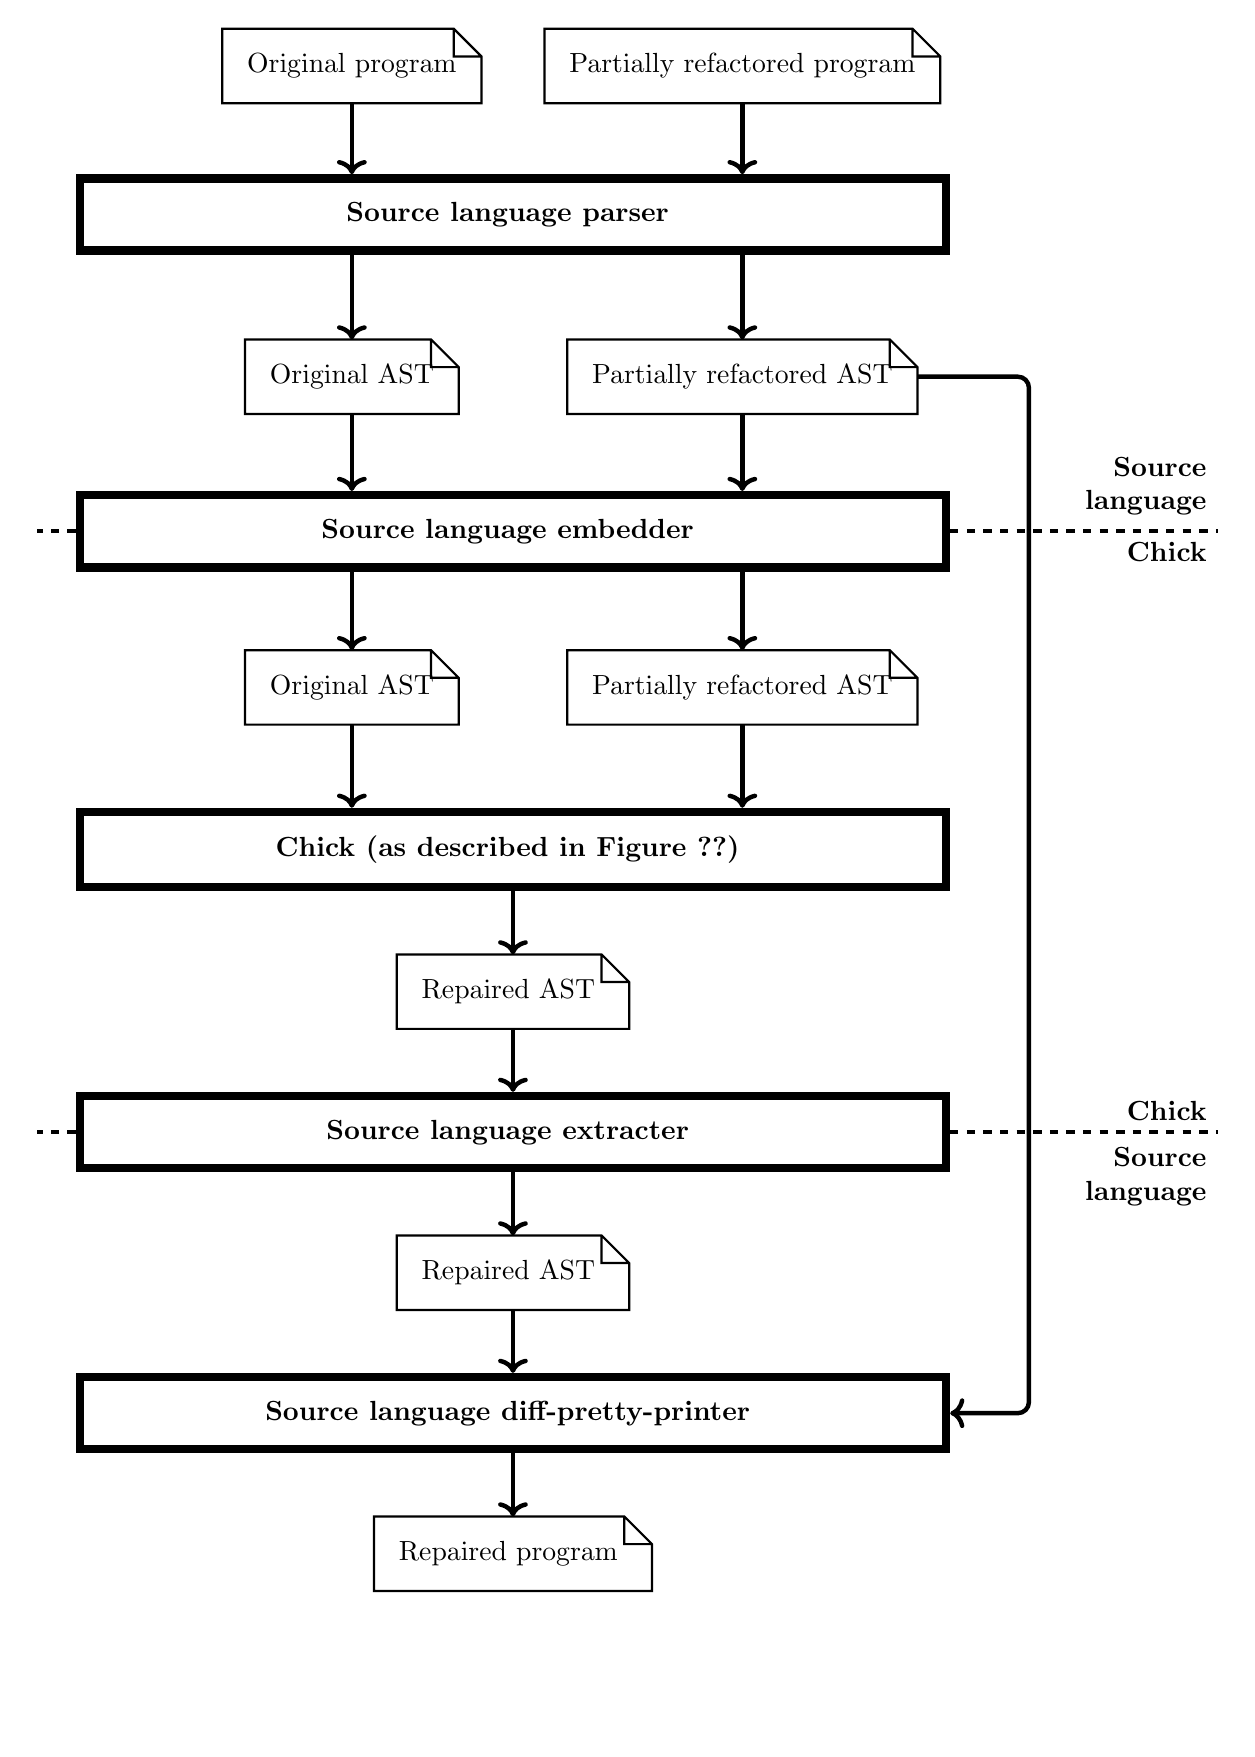
\begin{tikzpicture}[node distance=0.8cm]

    \tikzstyle{box} = [%
    align=center,
    draw=black,
    font=\bfseries,
    inner sep=2ex,
    line width=3pt,
    rectangle,
    %ultra thick,
    ];

    \tikzstyle{doc}=[%
    align=center,
    draw=black,
    shape=document,
    inner sep=2ex,
    shape=document,
    thick,
    ]

    %\draw [dotted,draw=black] (0,0) grid (15,22) rectangle (0,0);
    \node at (0,0)  (SW) { };
    \node at (15,0) (SE) { };

    \node[doc] at (4,21) (original-1) {Original program};
    \node[doc,right=of original-1] (modified-1) {Partially refactored program};
    \path (original-1) -- node (mid-1) {} (modified-1);

    \node[box,below=1.25cm of mid-1,minimum width=11cm] (parser) { Source language parser };

    \node[doc,below=3cm of original-1] (original-2) {Original AST};
    \node[doc,below=3cm of modified-1] (modified-2)
    {Partially refactored AST};

    \node[box,below=3cm of parser,minimum width=11cm] (embedder) { Source language embedder };

    \draw[dashed, ultra thick] (embedder.west) -- (embedder.west -| SW);
    \draw[dashed, ultra thick] (embedder.east) -- (embedder.east -| SE)
    node[above left,font=\bfseries]{\makecell[r]{Source\\language}}
    node[below left,font=\bfseries]{Chick}
    ;

    \node[doc,below=3cm of original-2] (original-3) {Original AST};
    \node[doc,below=3cm of modified-2] (modified-3)
    {Partially refactored AST};

    \node[box,below=3cm of embedder,minimum width=11cm] (chick)
    { Chick (as described in Figure~\ref{chick-workflow}) };

    \node[doc,below=of chick]      (repaired-1) { Repaired AST };
    \node[box,below=of repaired-1,minimum width=11cm] (extracter)
    { Source language extracter };

    \draw[dashed, ultra thick] (extracter.west) -- (extracter.west -| SW);
    \draw[dashed, ultra thick] (extracter.east) -- (extracter.east -| SE)
    node[above left,font=\bfseries]{Chick}
    node[below left,font=\bfseries]{\makecell[r]{Source\\language}}
    ;

    \node[doc,below=of extracter]  (repaired-2) { Repaired AST };
    \node[box,below=of repaired-2,minimum width=11cm] (printer)
    { Source language diff-pretty-printer };
    \node[doc,below=of printer]    (repaired-3) { Repaired program };

    \draw[->,ultra thick] (original-1.south) -- (original-1.south |- parser.north);
    \draw[->,ultra thick] (modified-1.south) -- (modified-1.south |- parser.north);

    \draw[->,ultra thick] (parser.south -| original-1.south) -- (original-2.north);
    \draw[->,ultra thick] (parser.south -| modified-1.south) -- (modified-2.north);

    \draw[->,ultra thick] (original-2.south) -- (original-2.south |- embedder.north);
    \draw[->,ultra thick] (modified-2.south) -- (modified-2.south |- embedder.north);

    \draw[->,ultra thick] (embedder.south -| original-2.south) -- (original-3.north);
    \draw[->,ultra thick] (embedder.south -| modified-2.south) -- (modified-3.north);

    \draw[->,ultra thick] (original-3.south) -- (original-3 |- chick.north);
    \draw[->,ultra thick] (modified-3.south) -- (modified-3 |- chick.north);

    \draw[->,ultra thick] (chick.south)      -- (repaired-1.north);
    \draw[->,ultra thick] (repaired-1.south) -- (extracter.north);
    \draw[->,ultra thick] (extracter.south)  -- (repaired-2.north);
    \draw[->,ultra thick] (repaired-2.south) -- (printer.north);
    \draw[->,ultra thick] (printer.south)    -- (repaired-3.north);

    \draw[->,rounded corners,ultra thick]
    (modified-2.east)
    -| ($(embedder.east)+(1,0)$)
    |- (printer.east);

    % \draw[->,rounded corners,ultra thick]
    % (original.east)
    % -- (guess.south |- original.east)
    % -- (guess.south)
    % ;

    % \draw[->,ultra thick] (modified.east) -- (guess.west);
    % \draw[->,ultra thick] (guess.east)    -- (guessed.west);

    % \draw[->,rounded corners,ultra thick]
    % (original.east)
    % -- (repair.south |- original.east)
    % -- (repair.south)
    % ;

    % \draw[->,ultra thick] (guessed.east) -- (repair.west);
    % \draw[->,ultra thick] (repair.east)  -- (repaired.west);

    % \draw[->,ultra thick] (original.east)  -- (patch.west);
    % \draw[->,ultra thick] (repaired.south) -- (patch.north);
    % \draw[->,ultra thick] (patch.south)    -- (patched.north);

  \end{tikzpicture}

  \caption{\Coop{}'s workflow}~\label{fig:coop-workflow}

\end{figure}

\section{Embedding and extracting programs}\label{coop-embedding-extracting}

In order to embed a new language into \Chick{}, we simply need to add a
constructor to the constructor of our \coqinline{Vernacular} and
\coqinline{Term} types.  For instance, we added support for \OCaml{} with the
following extension:

\begin{grammar}
<vernacular> ::= \ %trick LaTeX
\alt … \hfill (same as in Section~\ref{chick-syntax-programs})
\alt \coqinline{OCamlStructureItem} <ocaml-structure-item>

<term> ::= \ %trick LaTeX
\alt … \hfill (same as in Section~\ref{chick-syntax-terms})
\alt \coqinline{OCamlExpression} <ocaml-expression>
\end{grammar}

Now, our \define{embedder} can inspect the incoming abstract syntax tree, and
decide to map constructs from the source language to \Chick{} constructs, when
it makes sense to do so, or store the constructs in the extra constructors when
there is no matching concept in \Chick{}.

For instance, in the \OCaml{} embedder, we map constructs such as \OCaml{}'s
(non-polymorphic) variants to our notion of inductive data types, since the
concepts match.  We can also map most simple expressions to our term type, but
complex features that we do not support (say, nested pattern matching) get put
aside in the \coqinline{OCamlExpression} constructor.

The \define{extracter} acts as an inverse of the embedder, mapping \Chick{}
constructs back to their source language counterpart.  Constructs that have
been stashed in one of our constructors for unsupported language features
are simply restored as is, and \Chick{} constructs are mapped back to the
source language construct they came from.

Unfortunately, we sometimes need to map different source language abstract
syntax trees to the same \Chick{} abstract syntax tree.  For instance,
using \OCaml{} as an example again, the following two functions:

\begin{minted}{ocaml}
let f x y = 42
let g x = fun y -> 42
let h = fun x -> fun y -> 42
\end{minted}

map to similar \Chick{} terms:

\begin{minted}{coq}
Definition f : _ := λ x, λ y, 42.
Definition g : _ := λ x, λ y, 42.
Definition h : _ := λ x, λ y, 42.
\end{minted}

In order to try and preserve surface-level syntax as much as possible, we would
like to attach metadata about such source language syntactic choices in \Chick{}
terms.  This goals seems at odds with our intent of making \Coop{} extensible,
but we can actually achieve this somewhat easily by using the so-called ``Trees
that grow'' technique employed by~\mycite{najd2017trees} for the Glasgow
\Haskell{} Compiler (GHC).  Using generalized algebraic data types (GADTs), and
type families, this technique allows us to build abstract syntax trees for
\Chick{} that can be decorated with arbitrary metadata, and use type-level
computations to determine what this metadata may be for different constructors
in different contexts.

For instance, we can solve the previous problem by attaching metadata about the
number of function arguments that are marked as parameters, as opposed to being
abstracted over.

\begin{minted}{haskell}
-- We declare the existence of a family of types for storing the
-- metadata attached to a Definition.
type family DefinitionMetadata ξ

-- We attach this metadata to the Definition contructor.
data Vernacular ξ
  = Definition (DefinitionMetadata ξ) (DefinitionData ξ)
  | …

-- We instantiate the family for the OCaml language with an
-- integer representing the number of explicit parameters.
type instance (DefinitionMetadata OCaml) = Int
\end{minted}

With this information attached to our \mintinline{haskell}{Definition} nodes,
the extracter can pick the appropriate form, so as to preserve the original
syntactic choice.

\begin{minted}{haskell}
extracterVernacularOCaml ∷ Vernacular 'OCaml → StructureItem
extracterVernacularOCaml (Definition metadata data) =
  -- Here, metadata ∷ Int, tells us how many parameters should
  -- be before the equal sign, vs. bound by a lambda
\end{minted}

Sometimes, \Chick{} might need to come up with a new datum, for which there is
no sensible metadata it could attach to it.  For such cases, using an optional
type for the metadata (say, \mintinline{haskell}{Maybe Int} instead of
\mintinline{haskell}{Int} here) allows us to avoid this issue.

Overall, this technique gives us great flexibility, as different languages will
need different metadata for the same concepts.  The language of choice is
carried throughout the \Chick{} pipeline as a type-level tag, using \Haskell{}'s
\mintinline{haskell}{DataKinds} extension.  This also means that, anywhere in
the pipeline, we can readily choose to inspect the tag and do something specific
based on it.  For now, we only use this technique to pick the appropriate parser
and pretty-printer, but it could also be used to change parts of the repair
algorithm if some language needs specific, distinct support.

\section{Optics to repair unknown language constructs}\label{coop-optics}

There is a big problem with the approach described in
Section~\ref{embedding-extracting}.  Consider the following \OCaml{} code:

\begin{minted}{ocaml}
type a = … (* some type definition *)

module SomeModule =
  struct
    type b = … (* some other type definition, depends on a *)
    let  f = … (* some function, depends on a *)
  end
\end{minted}

Our current implementation of \Chick{} does not have a notion of modules.
Therefore, \Coop{} has to stash away the whole module declaration in its
\coqinline{OCamlStructureItem}, and will provide no repair for it.  This is
unfortunate, because the module contains data type declarations, and function
declarations, all of which we know how to repair, and could attempt to, were
they visible.

We can find a solution to this problem using functional lenses.  \define{Lenses}
are an abstraction mechanism encompassing a pair of a getter and a setter for
some value within some datum.  They are often described in the simplified
version:

\begin{minted}{haskell}
data Lens s a = Lens
  { get ∷ s → a
  , set ∷ s → a → s
  }
\end{minted}

\noindent where \mintinline{haskell}{s} stands for the type of the store, or the
outer structure, and \mintinline{haskell}{a} stands for the type of the value
under focus.\footnote{Actual implementations of lenses are usually more complex,
with two additional parameters allowing the setter to output at a different
store type. Some instances also add a \mintinline{haskell}{Functor} constraint
to allow getting and setting in a functorial context.}

Lenses are useful because they are first-class, composable values that allow
modifying parts of a datum while ignoring the rest of it.  This matches quite
well with our goal: we wanted to zoom in on the inner parts of the module,
getting and setting the components of the module we understand, ignoring the
rest.  However, lenses only have one focus, whereas our data could contain
an arbitrary amount of components we might want to focus upon.

\define{Traversals} are a generalization of lenses with multiple foci.  They are
also an abstraction of a getter and a setter, except that they may operate on
multiple instances of the focus type within a datum.  In order to allow maximum
flexibility, traversals process the foci within an applicative functor.  Uniform
traversals over parameterized data structures can be automatically derived using
extensions like \Haskell{}'s \mintinline{haskell}{TemplateHaskell}, but in our
case, we will need to write our traversals manually.  This allows us to
specifically choose the order of the traversal, as well as selectively choose
whether some parts of data types should be traversed or not.  Let us see how we
can define such a traversal over \OCaml{} abstract syntax trees.  For this, we
will use type classes to capture data types that contain structures we are
interested in.  For the \OCaml{} language, we are interested in values of type
\mintinline{haskell}{Structure} (which correspond to our \coqinline{Vernacular}
data type), and values of type \mintinline{haskell}{CoreType} and
\mintinline{haskell}{Expression} (which correspond to our \coqinline{Term} data
type).

\begin{minted}{haskell}
class HasStructure t where
  structure ∷ Traversal' t Structure

class HasCoreType t where
  coreType ∷ Traversal' t CoreType

class HasExpression t where
  expression ∷ Traversal' t Expression
\end{minted}

We can then instantiate those classes for all of \OCaml{}'s abstract syntax tree
constructs, for instance:

\begin{minted}{haskell}
instance HasStructure ModuleExprDesc where
  structure f = case f of
    -- if something does not contain a Structure,
    -- we can skip it entirely:
    PmodIdent     i → PmodIdent <$> pure i
    -- if something contains a Structure right here,
    -- we can apply `f`
    PmodStructure s → PmodStructure <$> f s
    -- if something may contain Structures recursively,
    -- we keep traversing it
    PmodApply m1 m2 → PmodApply
                      <$> traverseOf structure f m1
                      <*> traverseOf structure f m2
    …
\end{minted}

\noindent Writing those instances is entirely systematic, so we believe it can
be automated using \Haskell{}'s \mintinline{haskell}{TemplateHaskell}
facilities, though we have not yet written such automation.

\subsection{Traversals over concrete syntax and functorial syntax}

Depending on how the abstract syntax tree of the source language has been
defined, there are actually two distinct ways of building those traversals.
They correspond to the following two ways of defining a data type of
''commands'' over a datatype of ''expressions'':

\begin{minted}{haskell}
-- Variant 1: concrete representation
data Language
  = DoSomething Language.Term
  | …

-- Variant 2: functorial representation
data LanguageF e
  = DoSomething e
  | …

type Language = LanguageF Language.Term
\end{minted}

With the \define{concrete representation}, the constructor
\mintinline{haskell}{DoSomething} may only ever contain values of type
\mintinline{haskell}{Language.Term}.  It is more rigid than the
\define{functorial representation}, wherein the type of expressions is
abstracted over.  In the functorial setting, one can instantiate the
\mintinline{haskell}{LanguageF} functor with different types, yielding a family
of concrete types.

With the functorial approach, \Coop{} can replace the source language's
expression type with its own type, essentially storing \Chick{} abstract syntax
trees within the source language's abstract syntax tree:

\begin{minted}{haskell}
data Vernacular f
  = …
  | ForeignLanguage (LanguageF f)
\end{minted}

In this case, \Chick{} can, given a traversal for \mintinline{haskell}{LanguageF
f}, transform all occurrences of \mintinline{haskell}{f} into
\mintinline{haskell}{Chick.Term}, and repair those using the applicative
functor.  While it is convenient to store our expressions within the original
abstract syntax tree, we are forced to replace all occurrences so that the types
match up.  Once all of this is done, we have the following endpoints:

\begin{minted}{haskell}
embed ∷ Vernacular Language.Term → Vernacular Chick.Term
embed = …

chick ∷ Vernacular Chick.Term → Vernacular Chick.Term
chick = …

extract ∷ Vernacular Chick.Term → Vernacular Language.Term
extract = …
\end{minted}

\noindent
and we can simply pipeline them together to obtain the resulting abstract syntax
tree, that must finally be processed by our pretty-printer (as described in
Section~\ref{coop-diff-pretty-printer}).

In the case of the concrete representation, because we cannot store \Chick{}
terms within the foreign language's abstract syntax tree, we must proceed with a
level of indirection: we can use an \define{indexed} traversal to extract a list
of all the values being traversed, turn those values into \Chick{} terms, repair
those \Chick{} terms, turn the repaired terms back into source language terms,
and finally reinsert those repaired terms in the proper locations using the
indexed traversal.  The process looks like the following partial code:

\begin{minted}{haskell}
itraverseLanguage ∷
  IndexedTraversal' Int Language.AST Language.Term
itraverseLanguage = …

getTerms ∷ Language.AST → [Language.Term]
getTerms = toListOf itraverseLanguage

-- From there, we do the following:
-- 1. map `embed`  to get a  [Chick.Term]    (unrepaired)
-- 2. map `repair` to get a  [Chick.Term]    (repaired)
-- 3. map `extract` to get a [Language.Term] (repaired)

insertRepairedTerms ∷
  [Language.Term] → Language.AST → Language.AST
insertRepairedTerms l =
  imapOf itraverseLanguage (λ index _ → l ‼ index)
\end{minted}

The indexed traversal allows us to know where to insert the repaired terms in
the original abstract syntax tree.

\subsection{Scope-aware traversals}

There remains yet another trouble with our traversals.  Consider the following
\OCaml{} code:

\begin{minted}{ocaml}
module SomeModule (A : ModuleTypeForA) =
  struct
    (* ... *)
  end
\end{minted}

Thanks to our traversals, we might be able to repair terms that appear within
this \OCaml{} functor\footnotemark{}.  Unfortunately, while glossing over the
\mintinline{ocaml}{module} construct, we also gloss over a binding construct,
introducing a binder \mintinline{ocaml}{A}.  This might create problems when
this module appears in an ambient context where some other variable
\mintinline{ocaml}{A} is bound.  In particular, if our repair algorithm is
trying to repair instances of the variable \mintinline{ocaml}{A}, it will,
erroneously, attempt to repair the local references to \mintinline{ocaml}{A},
mistaking them for references the outer \mintinline{ocaml}{A}.

\footnotetext{Note that \OCaml{} uses the term \emph{functor} to describe about
parameterized \emph{modules}, while, so far, this dissertation has been using
the term functor to describe functorial parameterized \emph{data types}.}

In order to avoid this issue, we can change our traversals so that they
accumulate bound variables as they traverse the source language abstract syntax
tree, and turn our focal points into a pair of the construct under focus, and
the list of binders it lives under.  With this information, we can easily alter
the term so that \Chick{} knows that those variables have been rebound.  This
can be achieved in two ways:

\begin{itemize}

  \item either by over-populating, before running the repair algorithm, its
local context with those binders (bound to an unknown type, represented as a
hole), and populating the local context diff with as many
$\MathMod{\MathSame{}}{…}$,

  \item or, by adding extraneous $\lambda$-abstractions to the term, and adding
as many extraneous $\MathModLam{\MathSame{}}{…}$ to its diff, and running the
repair algorithm in the current global environment and local context.  This
requires a post-processing pass to remove those extraneous lambdas from the
repaired term, before injecting it back into its abstract syntax tree.

\end{itemize}

\section{Diff-aware pretty-printing}\label{coop-diff-pretty-printer}

So far, we have explained how we can embed the constructs and binding structure
from the abstract syntax tree of some arbitrary source language, repair those
constructs as part of our core language, and then extract the repaired
constructs back into an abstract syntax tree for the original language.
However, we need to repair the concrete syntax of the original program, not just
the abstract syntax tree.

While we could just call a naive pretty-printer with the final abstract syntax
tree, there is a high chance that doing so would interfere with the layout of
the original code, unless we somehow stored enough information to reproduce the
exact original layout.  In order to minimize our impact on the concrete syntax
of the program, we can instead try to only modify those parts of the concrete
syntax that need being altered.

To do so, we need the abstract syntax tree of the source language to contain
location information about the provenance of its nodes.  This requirement is not
hard to satisfy: we expect most languages to have parsers that produce such
information, if only to be able to indicate error locations.  Now, when we
obtain the repaired source abstract syntax tree, we can simply follow a
simultaneous recursive descent through the original and repaired trees.  At any
point where they differ, we can:

\begin{itemize}

  \item obtain the source span for the text to be replaced from the original
tree,

  \item obtain the replacement text by pretty-printing the node from the
repaired tree.

\end{itemize}

\noindent
Then, we can graft the pretty-printed repaired term in place of the original
text span.  If the language is indentation-sensitive, we might need to be more
clever, figuring out the level of indentation, and hanging the replacement
text at that depth.

We can also come up with extra quality of life improvements, such as retaining
and lifting the comments from the deleted span, so that no comment is lost in
the repair.  Repairs can also be processed sequentially, with a human in the
loop, so that repair suggestions are reviewed by the user before being applied,
for instance, by using a merging tool such as the ones provided for version
control systems.


This chapter is, in part, currently being prepared for submission for
publication of the material.

\chapter{Related work}

TODO

\chapter{Future work}

In this chapter, we will go over several potential ways to extend \Chick{} and
\Coop{} in the future.

\section{Avoiding problematic binders using scope sets}

TODO

\section{Repairing tactic scripts}

Using the same methodology we used to repair programs and terms, we have
considered repairing proof scripts written in a tactic language like \Ltac{}.
The problem with \Coq{} tactics is that their effect depends on what is in
context when the tactic is called, making them hard to reason about statically.
For instance, the \coqinline{intros} tactic inspects the current sub-goal, and
introduces as many universally quantified variables from the sub-goal as it can.
To do so, it has to come up with names for those variables, yet the user never
explicitly passes those names.  Instead, the algorithm chooses suitable, fresh
names, using the names of the variables as they appear in the sub-goal (when
their quantification is explicitly named), or picking some fresh name.

For instance, if your current goal is:

\begin{minted}[linenos=false]{coq}
nat → nat → nat → nat
\end{minted}

\noindent%
%
and you run \coqinline{intros}, the following names will be added to your
context:

\begin{minted}[linenos=false]{coq}
H, H0, H1 : nat
\end{minted}

\noindent%
%
This makes tactic scripts complicated to repair, as there is no lexical binding
position for those automatically introduced names.  In order to repair tactic
scripts, we \emph{must} be able to replay them.  This can only be done outside
the tool if the tactic language has well-defined semantics.  Unfortunately,
\Ltac{} is a very complicated tactic script, and formalizing its semantics is
still an open-ended problem.

Had we done so, we could hope to repair tactics by replaying them, and computing
diffs for the proof context, just like we did for our global environment and
local context when repairing terms.  The problem is very interesting, as a
change in the number of constructors of a data type can have drastic changes in
the structure of a proof.  We have started working on a prototype, toying with
repairing a tactic language that only provides tactics like \coqinline{intro}
and \coqinline{destruct}, but we don't have a proper prototype for those yet.

\section{Integrating code diffs in version control systems}

An equally ambitious goal could be to treat our diffs, that is, first-class
values that represent the intent of changes made to a program, the same way we
treat the code of the program.  For instance, as a program evolves, we keep a
published index on the changes made to it using a version control system.  We
can envision a diff-aware version system wherein diffs are also published.

Consider a use case where Ada is publishing a software library that Bertrand
depends upon for his project.  When Ada decides to make a breaking change to her
library, she could perform the change by using a diff-based repair algorithm
like the one we present.  When the repair is finished, she has a complete,
structural diff, that captures exactly all of the changes that have happened to
the library.  Ada can publish this diff, alongside the new code, to her public
version control system.  Bertrand can update his dependency to Ada's new
version, but he needs to update his client code to adapt to the changes made by
Ada.  Thanks to the published diffs, Bertrand could also run a repair algorithm
over his code, automating much of the necessary code changes needed to stay
compatible with Ada's library.

Of course, this workflow would need to be extremely polished to convince both
users to opt in.  In particular, we would definitely want a strong diff guessing
algorithm, like the one presented in Section~\ref{chick-guess}, and would need a
nice way of presenting different guesses to the programmer so that they can
safely pick the choice that best matches their intent.

%\input{future-ide}


\appendix

\chapter{\PeaCoq{} A-B study post-study survey}~\label{appendix-peacoq-a-b-study}

We report the qualitative feedback obtained via a questionnaire given after the
A-B study described in Section~\ref{peacoq-a-b-study}.  We indicate participants
anonymously as $Xp_{i}$ where $X$ stands for the study group ($A$ being the
\define{control group}, $B$ being the group testing our tool), $p$ stands for a
given pair of participants, and $i$ distinguishes between the two participants
in a pair.

We report participants' answers as is: we do fix typos, but do not alter their
phrasing or grammatical structures whatsoever.

\clearpage

\noindent
\begin{tabularx}{\linewidth}{@{}cX@{}}
  \toprule
  Participant & \multicolumn{1}{c}{
    \textbf{In your own words, describe what you did today.}
  } \\ \midrule
  $A1_{1}$ & Proved several theorems in a pair using an interactive proof assistant. \\
  $A1_{2}$ & \begin{enumerate*} \item Proved some set and logic and operation lemmas and theorems. \item Used a new tool to write the proofs. \end{enumerate*} \\
  $A2_{1}$ & Tried to understand \Coq{} by using an entire IDE and write some proofs. \\
  $A2_{2}$ & We used a proof assistant to prove theorems about lists and their properties. \\
  $A3_{1}$ & We used the theorem prover to prove that the functions of code did what they meant to in all cases. \\
  $A3_{2}$ & Today I learned about the \Coq{} theorem proving language.  After an introduction, I worked in a pair to solve various theorems for lists of natural numbers, and maps. \\
  $A4_{1}$ & Use an automated theorem prover to prove basic facts in data structures and logic. \\
  $A4_{2}$ & We used a tool that could define predicates, types and prove various properties about them. \\
  $A5_{1}$ & We learned a little about basic proofs in \Coq{} then applied what we learned in the exercises. \\
  $A5_{2}$ & I used a proof assistant to prove several simple mathematical theorems. \\
\end{tabularx}{\parfillskip=0pt\par}

\clearpage

\noindent
\begin{tabularx}{\linewidth}{@{}cX@{}}
  \toprule
  Participant & \multicolumn{1}{c}{
    \textbf{In your own words, describe what you did today.}
  } \\ \midrule
  $B1_{1}$ & I used a graphical tool to prove several invariants about functions/data structures in a given language (\Coq{}). \\
  $B1_{2}$ & Proved some special cases of inferences from new definitions using induction and other primitive proof techniques.  Use already proved theorems in future proofs. \\
  $B2_{1}$ & I used a programming language tool to prove various constructs. \\
  $B2_{2}$ & Proved a bunch of simple theorems about functions working on lists. \\
  $B3_{1}$ & Use \Coq{} to prove a theorem.  Reasoning the steps and select what makes sense from the options given by the tool. \\
  $B3_{2}$ & We were trying to use \PeaCoq{} to prove a bunch of theorems by exploring all the possible strategies, such as induction, transformation, simplification, etc. \\
  $B4_{1}$ & We used a graphical version of an interactive proof assistant to prove some theorems involving list operations. \\
  $B4_{2}$ & Proved some functions using \PeaCoq{}. \\
  $B5_{1}$ & We used the \PeaCoq{} web editor interface to prove theorems on pieces of code via \Coq{}.  First we were given an introduction to \Coq{} combined with a tutorial on using the tool, and then we worked in pairs on a series of example of proofs/theorems. \\
  $B5_{2}$ & I used a modified version of the \Coq{} proof assistant to prove things about lists and functions over them. \\
  \bottomrule
\end{tabularx}{\parfillskip=0pt\par}

\clearpage

\noindent
\begin{tabularx}{\linewidth}{@{}cX@{}}
  \toprule
  Participant & \multicolumn{1}{c}{
    \textbf{What did the experience today remind you of?}
  } \\ \midrule
  $A1_{1}$ & Learning to program for the first time. Lots of brute-forcing and trying things that worked in the past to see if they would work in a new context. \\
  $A1_{2}$ & Using induction in high school/undergrad and trying to draw insights from proving the base case to apply to the general case. \\
  $A2_{1}$ & Today was quite unique but I felt like writing functional programs since I tried to prove my implementation there too. \\
  $A2_{2}$ & It reminded me of working on large code bases where certain things appear to work by magic.  Fixes/proofs were performed with little fundamental understanding. \\
  $A3_{1}$ & Taking a programming languages class, since the constructs are all the same. \\
  $A3_{2}$ & Today's experience reminded me of an intro to algorithms course. \\
  $A4_{1}$ & Proving mathematical theorems for research. \\
  $A4_{2}$ & Liquid types in Haskell.  Mathematical induction. \\
  $A5_{1}$ & Learning programming in school and proofs in math classes. \\
  $A5_{2}$ & It reminded me of pen-and-paper proofs. \\
\end{tabularx}{\parfillskip=0pt\par}

\clearpage

\noindent
\begin{tabularx}{\linewidth}{@{}cX@{}}
  \toprule
  Participant & \multicolumn{1}{c}{
    \textbf{What did the experience today remind you of?}
  } \\ \midrule
  $B1_{1}$ & Playing a logical/exploration game. \\
  $B1_{2}$ & \begin{enumerate*} \item Writing unit tests for corner cases. \item Giving a systematic proof covering all cases. \end{enumerate*} \\
  $B2_{1}$ & It reminded me of safe programming techniques in the way that if we can prove that our constructs work, there shouldn't be any problems at run-time. \\
  $B2_{2}$ & Functional programming and reasoning about it. \\
  $B3_{1}$ & First time to learn formal proof stuff. \\
  $B3_{2}$ & Decision tree. \\
  $B4_{1}$ & It reminded me of a puzzle game in which you have to reach a target and can use as keys some of the facts you encounter on your way there. \\
  $B4_{2}$ & Proving technique classes. \\
  $B5_{1}$ & The \inferrule{ \text{rules} \\\\ \text{rules} \\\\ \text{rules} }{ statement } format reminded me of constructions I have seen in computer science papers that have not formally learned about.  The theorems we were proving, e.g. \safecoqinline{concat xs nil = xs}, reminded in a different/more powerful direction (but requiring manual work to prove). \\
  $B5_{2}$ & Analysis class, proving simple-seeming things about math was similarly harder than it looked. \\
  \bottomrule
\end{tabularx}{\parfillskip=0pt\par}

\clearpage

\noindent
\begin{tabularx}{\linewidth}{@{}cX@{}}
  \toprule
  Participant & \multicolumn{1}{c}{
    \textbf{Did you understand all the proofs you completed?}
  } \\ \midrule
  $A1_{1}$ & No. \\
  $A1_{2}$ & No.  We figured out that there were some hammers which we should keep using (\safecoqinline{simpl}, \safecoqinline{reflexivity}, \safecoqinline{rewrite}).  They mostly made sense but we didn't spend time to understand the exact changes they made. \\
  $A2_{1}$ & Most of them.  Especially the last ones were quite confusing. \\
  $A2_{2}$ & Not entirely.  While I had conceptual knowledge of what was happening, I didn't understand it holistically. \\
  $A3_{1}$ & Yes. \\
  $A3_{2}$ & Yes. \\
  $A4_{1}$ & Yes. \\
  $A4_{2}$ & Yes. \\
  $A5_{1}$ & Yes. \\
  $A5_{2}$ & Yes. \\
\end{tabularx}{\parfillskip=0pt\par}

\clearpage

\noindent
\begin{tabularx}{\linewidth}{@{}cX@{}}
  \toprule
  Participant & \multicolumn{1}{c}{
    \textbf{Did you understand all the proofs you completed?}
  } \\ \midrule
  $B1_{1}$ & Yes. \\
  $B1_{2}$ & Yes. \\
  $B2_{1}$ & Yes, the only one that I had trouble with was \safecoqinline{destruct}. \\
  $B2_{2}$ & No. \\
  $B3_{1}$ & No.  Sometimes it is magically done. \\
  $B3_{2}$ & No, but most of them. \\
  $B4_{1}$ & Yes (at least on a second closer inspection). \\
  $B4_{2}$ & No. \\
  $B5_{1}$ & For the most part.  The last exercise (\safecoqinline{In_concat_left}) had me a bit confused on how \safecoqinline{destruct} worked/what it did.  Once that clicked for me, what we were doing there made sense. \\
  $B5_{2}$ & I think so? \\
  \bottomrule
\end{tabularx}{\parfillskip=0pt\par}

\noindent
\begin{tabularx}{\linewidth}{@{}cX@{}}
  \toprule
  Participant & \multicolumn{1}{c}{
    \textbf{Did you find the tool useful for achieving the tasks?}
  } \\ \midrule
  $A1_{1}$ & Error messages were mostly helpful sometimes. Sort of. Clear when something didn't work. \\
  $A1_{2}$ & Yes.  Because it would stop me from trying to use wrong rules.  Also because I could follow from one lemma to another in most cases. \\
  $A2_{1}$ & \begin{enumerate*} \item Has a simple, clean UI \item Doesn't require anything other than a browser. \end{enumerate*} \\
  $A2_{2}$ & A little.  It provided confidence that the task was completed correctly. \\
  $A3_{1}$ & Yes.  I like how the right side always showed the next goal, in that it was easy to focus on one statement at a time. \\
  $A3_{2}$ & Yes, very. \\
  $A4_{1}$ & Yes, it was pretty self-explanatory.  Inline code and comments very helpful. \\
  $A4_{2}$ & Yes. \\
  $A5_{1}$ & Yes, the step by step approach was helpful to visualize how the proof was coming along.  It also helped with trial and error. \\
  $A5_{2}$ & Highlighting, previous/next were extremely useful.  The information snippets would be useful if I weren't the proof author. \\
\end{tabularx}{\parfillskip=0pt\par}

\clearpage

\noindent
\begin{tabularx}{\linewidth}{@{}cX@{}}
  \toprule
  Participant & \multicolumn{1}{c}{
    \textbf{Did you find the tool useful for achieving the tasks?}
  } \\ \midrule
  $B1_{1}$ & The tool was very useful, specifically: \begin{enumerate*} \item Highlighting the diffs was helpful to explain what each tactic does, \item Having all the options available to apply was helpful for a novice who doesn't know what the available tactics are. \end{enumerate*} \\
  $B1_{2}$ & Yes. \\
  $B2_{1}$ & It definitely helped in showing the paths you could take in a proof, which is helpful if you can't think of them on the spot. \\
  $B2_{2}$ & I proved things without having to think too hard about it. \\
  $B3_{1}$ & \begin{enumerate*} \item As an inexperienced learner, I even don't know how to start a proof, but the tool gives me the guidance to do this. \item After some time, when you get familiar with it, there exists some patterns to find the correct solution. \end{enumerate*} \\
  $B3_{2}$ & I think it's useful.  But it is hard to say ``how'' useful it is for two reasons: \begin{enumerate*} \item I'm not aware of any order tools, \item the problems are actually simple and intuitive to prove manually. \end{enumerate*} \\
  $B4_{1}$ & \begin{enumerate*} \item Provided a broad overview of the available options (some perhaps ``counter-intuitive'' options that I might have thought of were presented right away), \item fewer keystrokes \item visual diffs are very useful for calculating how bigger / smaller our target is. \end{enumerate*} \\
  $B4_{2}$ & I wouldn't be able to achieve the tasks on my own, but that's probably because I have no idea how to prove those things. \\
  $B5_{1}$ & Yes, absolutely.  The tree interface made exploring possible tactics and seeing the results very quick and easy.  I've never actually used \Coq{} or anything like it before but with this interface I was able to get up to speed pretty quickly. \\
  $B5_{2}$ & I didn't have to already know/remember the set of options, and it was useful to get a preview of what each one would do. \\
  \bottomrule
\end{tabularx}{\parfillskip=0pt\par}

\clearpage

\noindent
\begin{tabularx}{\linewidth}{@{}cX@{}}
  \toprule
  Participant & \multicolumn{1}{c}{
    \textbf{Do you have suggestions on how to improve the tool you used today?}
  } \\ \midrule
  $A1_{1}$ & Backing up through a \safecoqinline{Qed.} backs up the entire proof.  Would prefer to step back one tactic at a time like during the proof.  Right-hand pane sometimes not wide enough to see everything.  Primitive sub-string matching to suggest rewrites would be useful. \\
  $A1_{2}$ & \begin{enumerate*} \item It should stop me from going down useless proof steps even though the rules apply. \item It should stop me from going in circles by warning (we are not sure we did that but came close). \item Difficult to translate intuition from base case to general case.  Had to use pen-and-paper at times to write small examples. \end{enumerate*} \\
  $A2_{1}$ & \begin{enumerate*} \item Missing some keyboard shortcuts. \item Having a pane which shows previous proofs would be quite helpful. \end{enumerate*} \\
  $A2_{2}$ & I had little confidence that I understood what was happening.  Completing the same proofs later would likely result in similar trial and error.  The only thing I was learning was the sort of patterns that proofs took on.  Variable names were confusing and hard to work with. \\
  $A3_{1}$ & \safecoqinline{each} should be syntax-highlighted. \\
  $A3_{2}$ & Adding auto-complete would be nice and a command list. \\
  $A4_{1}$ & Previously-proved functions were difficult to find/see when scrolling up.  I could see this being a major problem for anything complex.  Could be solved with a better interface e.g.\ in an IDE.\@Not related to the software, but there's a tendency to avoid planning and just react to results of \safecoqinline{simpl}, \safecoqinline{rewrite}, etc. \\
  $A4_{2}$ & \begin{enumerate*} \item Bugs when we were using Firefox instead of Chrome.  Tool wouldn't revert steps correctly. \item Auto-completion of previously-defined rewrite theorems \end{enumerate*} \\
  $A5_{1}$ & Flip Next and Previous in the GUI. \\
  $A5_{2}$ & Some sort of search (``I want to use this'') would be handy.  The coloring breaks on exceptions. \\
\end{tabularx}{\parfillskip=0pt\par}

\clearpage

\noindent
\begin{tabularx}{\linewidth}{@{}cX@{}}
  \toprule
  Participant & \multicolumn{1}{c}{
    \textbf{Do you have suggestions on how to improve the tool you used today?}
  } \\ \midrule
  $B1_{1}$ & \begin{enumerate*} \item Highlight the border of the sub-window (code/proof) that has keyboard focus, \item When deep in a proof tree, I kept forgetting what induction hypothesis I had accumulated so far (and I think I didn't always see them in the current goal).  It would be useful to somehow get reminded of what invariants/induction hypothesis I had accumulated. \end{enumerate*} \\
  $B1_{2}$ & A first time user might find it difficult to switch between cases using ``['' and ``]''.  Some syntax in languages were not straightforward, for instance \safecoqinline{fold}.  Syntax of \safecoqinline{map} functions were clear. \\
  $B2_{1}$ & Maybe look ahead and see if some paths don't lead to solutions. \\
  $B2_{2}$ & \emph{No answer provided.} \\
  $B3_{1}$ & \emph{No answer provided.} \\
  $B3_{2}$ & I guess it's definitely helpful if the tool can automatically probing some paths without clicking. \\
  $B4_{1}$ & \begin{enumerate*} \item Trivialize options that lead to the target in one to two steps. \item On the fly explanation of what the operators do. \end{enumerate*} \\
  $B4_{2}$ & It crashes when you hit the left button three or four times quickly. \\
  $B5_{1}$ & There was that one bug that we ran into a few times: going back causing the editor to crash, that made us lose progress a few times.  \begin{enumerate*} \item An auto-save feature would be appreciated as a guard against this (could use e.g. Local Storage API), \item A way to ``bookmark'' and jump back to points in the tree would be appreciated, perhaps also some highlights of previously-explored paths? \end{enumerate*} \\
  $B5_{2}$ & A minor one: \safecoqinline{intros.} should be option one (instead of \safecoqinline{intro x.}) since it always seems like the right start. \\
  \bottomrule
\end{tabularx}{\parfillskip=0pt\par}

\noindent
\begin{tabularx}{\linewidth}{@{}cX@{}}
  \toprule
  Participant & \multicolumn{1}{c}{
    \textbf{Explain in your own word what the \safecoqinline{each} tactic does.}
  } \\ \midrule
  $A1_{1}$ & Splits up an \safecoqinline{AND} so each side can be proven separately. \\
  $A1_{2}$ & Split/divides a proof of an \safecoqinline{AND} expression into two different proof exercises. \\
  $A2_{1}$ & Used to prove both paths of a theorem (conjunction) with two parts. \\
  $A2_{2}$ & Splits a logical \safecoqinline{and} into subgoals for each expression. \\
  $A3_{1}$ & Follow both branches of an \safecoqinline{AND}, since both must be proven. \\
  $A3_{2}$ & Selects the terms from both sides of an \safecoqinline{AND}. \\
  $A4_{1}$ & Enumerates all cases in a conjunction. \\
  $A4_{2}$ & Divides the \safecoqinline{AND} predicate into two sub-problems so we can prove each separately. \\
  $A5_{1}$ & Splits an \safecoqinline{and} into each side so they can be proved separately. \\
  $A5_{2}$ & Split conjunction. \\
\end{tabularx}{\parfillskip=0pt\par}

\clearpage

\noindent
\begin{tabularx}{\linewidth}{@{}cX@{}}
  \toprule
  Participant & \multicolumn{1}{c}{
    \textbf{Explain in your own word what the \safecoqinline{each} tactic does.}
  } \\ \midrule
  $B1_{1}$ & For a goal \safecoqinline{A /\ B} introduces 2 subgoals \safecoqinline{A} and \safecoqinline{B}. \\
  $B1_{2}$ & Prove each child tree is correct. \\
  $B2_{1}$ & Applies some function to all elements in a set. \\
  $B2_{2}$ & Prove all sub-trees. \\
  $B3_{1}$ & Every element in a collection. \\
  $B3_{2}$ & Try to prove each case. \\
  $B4_{1}$ & Apply action to all elements of a collection. \\
  $B4_{2}$ & ? \\
  $B5_{1}$ & When you have \safecoqinline{A /\ B}, you need to prove both \safecoqinline{A} and \safecoqinline{B}, so split, doing \safecoqinline{A} and then \safecoqinline{B}. \\
  $B5_{2}$ & Splits an \safecoqinline{A /\ B} goal into separate \safecoqinline{A} and \safecoqinline{B} goals. \\
  \bottomrule
\end{tabularx}{\parfillskip=0pt\par}

\clearpage

\noindent
\begin{tabularx}{\linewidth}{@{}cX@{}}
  \toprule
  Participant & \multicolumn{1}{c}{
    \textbf{Explain in your own word what the \safecoqinline{intro} tactic does.}
  } \\ \midrule
  $A1_{1}$ & Fixes some \safecoqinline{forall} value. \\
  $A1_{2}$ & Introduces the different variables in the expression. \\
  $A2_{1}$ & Instantiates the \safecoqinline{forall} variables. \\
  $A2_{2}$ & Do it first thing? \\
  $A3_{1}$ & Apply a \safecoqinline{foreach}. \\
  $A3_{2}$ & Provides the types for the theorem we are proving. \\
  $A4_{1}$ & Instantiates a placeholder variable under a universal quantifier. \\
  $A4_{2}$ & Infers already known information from the setup to give us known or assumed values. \\
  $A5_{1}$ & List names of variables in \safecoqinline{forall} and hypotheses. \\
  $A5_{2}$ & Instantiate \safecoqinline{forall}. \\
\end{tabularx}{\parfillskip=0pt\par}

\clearpage

\noindent
\begin{tabularx}{\linewidth}{@{}cX@{}}
  \toprule
  Participant & \multicolumn{1}{c}{
    \textbf{Explain in your own word what the \safecoqinline{intro} tactic does.}
  } \\ \midrule
  $B1_{1}$ & Given a \safecoqinline{forall x, p(x)} goal, make up a new variable name \safecoqinline{x} and introduce it and make \safecoqinline{p(x)} (with that specific \safecoqinline{x}) the current sub-goal. \\
  $B1_{2}$ & Introduce (or define) the variables used in proof. \\
  $B2_{1}$ & Introduces all the components of your proof in order to use them. \\
  $B2_{2}$ & Introduce quantified variables (i.e. give them a name). \\
  $B3_{1}$ & Extend the original theorem to an easy-to-understand format. \\
  $B3_{2}$ & Give a start point. \\
  $B4_{1}$ & Add facts to your assumptions. \\
  $B4_{2}$ & ? \\
  $B5_{1}$ & Take the names from the \safecoqinline{forall} and put them in the usable rule environment.  It was sort of unclear to me why we needed to do this explicitly every time. \\
  $B5_{2}$ & Equivalent of the mathematician's ``fix'', gets rid of \safecoqinline{forall}. \\
  \bottomrule
\end{tabularx}{\parfillskip=0pt\par}

\clearpage

\noindent
\begin{tabularx}{\linewidth}{@{}cX@{}}
  \toprule
  Participant & \multicolumn{1}{c}{
    \textbf{Explain in your own word what the \safecoqinline{induction} tactic does.}
  } \\ \midrule
  $A1_{1}$ & Allows case analysis over inductive types. \\
  $A1_{2}$ & Applies induction the variable mentioned as parameter and breaks the proof into base case and general case. \\
  $A2_{1}$ & To use induction on a given variable.  Proof by cases analysis. \\
  $A2_{2}$ & Perform induction with two steps/goals: base case + inductive case. \\
  $A3_{1}$ & Break a step into its base case(s) and recursive case(s). \\
  $A3_{2}$ & Performs induction on an element. \\
  $A4_{1}$ & Breaks a logical statement universally quantifying over a variable \safecoqinline{x}, into cases based on \safecoqinline{match}. \\
  $A4_{2}$ & Performs mathematical induction.  Divides into base case, induction case.  Assumes hypothesis. \\
  $A5_{1}$ & Breaks a list into the base case and induction step. \\
  $A5_{2}$ & Induct over recursive variable. \\
\end{tabularx}{\parfillskip=0pt\par}

\clearpage

\noindent
\begin{tabularx}{\linewidth}{@{}cX@{}}
  \toprule
  Participant & \multicolumn{1}{c}{
    \textbf{Explain in your own word what the \safecoqinline{induction} tactic does.}
  } \\ \midrule
  $B1_{1}$ & If \safecoqinline{x} is of a given type (like ML algebraic types), do a case analysis for each of the constructors of the type.  If one of them is recursive, introduce a hypothesis for its sub-part, and use it to prove the statement for the larger goal. \\
  $B1_{2}$ & Split into two branches: base case and induction case.  Introduce a hypothesis argument called \safecoqinline{IH} which can be invoked later in the proof. \\
  $B2_{1}$ & Proves that some function works for arbitrary element. \\
  $B2_{2}$ & Start an inductive proof (base case + step). \\
  $B3_{1}$ & \begin{enumerate*} \item Base case, \item Induction... \end{enumerate*} \\
  $B3_{2}$ & It's just ``induction'' we do... counting base case, inductive hypothesis, inductive steps. \\
  $B4_{1}$ & Do structural induction of a... \\
  $B4_{2}$ & Proof by induction. \\
  $B5_{1}$ & Case analysis: break e.g. a list into \safecoqinline{nil} and \safecoqinline{cons}, and branch along each path with an additional inductive hypothesis, proving each path (one for each possible value/case) proves the overall theorem. \\
  $B5_{2}$ & Splits a goal involving a recursively-defined data type into a base case and an inductive step goal (in the latter, you get the inductive hypothesis in the environment). \\
  \bottomrule
\end{tabularx}{\parfillskip=0pt\par}

\clearpage

\noindent
\begin{tabularx}{\linewidth}{@{}cX@{}}
  \toprule
  Participant & \multicolumn{1}{c}{
    \textbf{Explain in your own word what the \safecoqinline{reflexivity} tactic does.}
  } \\ \midrule
  $A1_{1}$ & Used when x = x. \\
  $A1_{2}$ & Comparing an expression with itself is true. \\
  $A2_{1}$ & Used to prove equality when both sides of the equality is the same (or very similar after simplifying). \\
  $A2_{2}$ & Attempt to reconcile an equality. \\
  $A3_{1}$ & When you have \safecoqinline{x = x}, call that step finished and move on to the next. \\
  $A3_{2}$ & Simplifies like expressions on both sides of the equality. \\
  $A4_{1}$ & Uses the tautological identity to prove trivial equalities.  Also does \safecoqinline{simpl}. \\
  $A4_{2}$ & \safecoqinline{A == A}. \\
  $A5_{1}$ & Simplifies and accepts if both sides are the same. \\
  $A5_{2}$ & Apply functions, find structural equality. \\
\end{tabularx}{\parfillskip=0pt\par}

\clearpage

\noindent
\begin{tabularx}{\linewidth}{@{}cX@{}}
  \toprule
  Participant & \multicolumn{1}{c}{
    \textbf{Explain in your own word what the \safecoqinline{reflexivity} tactic does.}
  } \\ \midrule
  $B1_{1}$ & \safecoqinline{x = x} is trivially true. \\
  $B1_{2}$ & \safecoqinline{a = a}.  Also simplifies based on definition of types. \\
  $B2_{1}$ & Two things are equivalent. \\
  $B2_{2}$ & Check if two things are equal. \\
  $B3_{1}$ & \safecoqinline{x = x}. \\
  $B3_{2}$ & Trivial equivalence. \\
  $B4_{1}$ & Use the reflexive property (along with some simplification). \\
  $B4_{2}$ & Checks if two things are the same. \\
  $B5_{1}$ & Prove \safecoqinline{a = a} for some \safecoqinline{a}. \\
  $B5_{2}$ & Proves \safecoqinline{x = x} (also performs simple simplifications). \\
  \bottomrule
\end{tabularx}{\parfillskip=0pt\par}

\noindent
\begin{tabularx}{\linewidth}{@{}cX@{}}
  \toprule
  Participant & \multicolumn{1}{c}{
    \textbf{Explain in your own word what the \safecoqinline{rewrite} tactic does.}
  } \\ \midrule
  $A1_{1}$ & Used to pull in some fact proven earlier. \\
  $A1_{2}$ & Uses the rule provided to find a component in LHS/RHS (depending on arrow) and modify it (as per the rule). \\
  $A2_{1}$ & Uses a rule to rewrite a part of the proof. \\
  $A2_{2}$ & Pattern-match and replace. \\
  $A3_{1}$ & Rewrite the current step with a specified function. \\
  $A3_{2}$ & Applies an equality to your current goal or sub-goal. \\
  $A4_{1}$ & Pattern-match part of an expression using a (inductive) hypothesis in scope. \\
  $A4_{2}$ & Substitution. \\
  $A5_{1}$ & Replaces one side of an expression with the other. \\
  $A5_{2}$ & Replace equal terms. \\
\end{tabularx}{\parfillskip=0pt\par}

\clearpage

\noindent
\begin{tabularx}{\linewidth}{@{}cX@{}}
  \toprule
  Participant & \multicolumn{1}{c}{
    \textbf{Explain in your own word what the \safecoqinline{rewrite} tactic does.}
  } \\ \midrule
  $B1_{1}$ & Use a previous lemma/induction hypothesis to transform some terms. \\
  $B1_{2}$ & Replace parts of LHS, RHS, using the theorems proved earlier. \\
  $B2_{1}$ & Use previous lemma or theorems to modify the construct. \\
  $B2_{2}$ & Use previously proven things to rewrite the expression. \\
  $B3_{1}$ & Rewrite some formulas to ones that are closer to the proof's target.  Better to utilize the existing hypothesis. \\
  $B3_{2}$ & Transformation. \\
  $B4_{1}$ & Use some rewrite property applied to parts of your expressions. \\
  $B4_{2}$ & Replaces a pattern in the text. \\
  $B5_{1}$ & Use a theorem/inductive hypothesis/other rewrite rule to transform part of the current node and continue with the proof. \\
  $B5_{2}$ & ``Substitution'' or ``plugging int''. \\
  \bottomrule
\end{tabularx}{\parfillskip=0pt\par}

\clearpage

\noindent
\begin{tabularx}{\linewidth}{@{}cX@{}}
  \toprule
  Participant & \multicolumn{1}{c}{
    \textbf{Explain in your own word what the \safecoqinline{goright} tactic does.}
  } \\ \midrule
  $A1_{1}$ & Tells proof assistant I'm about to prove the right-hand side of an \safecoqinline{OR}. \\
  $A1_{2}$ & Choose the right-side expression in a combination of Boolean expressions. \\
  $A2_{1}$ & To prove the right part of an \safecoqinline{OR} expression. \\
  $A2_{2}$ & Take a goal with a logical \safecoqinline{or} and solve only the right sub-expression. \\
  $A3_{1}$ & Follow the right branch of an \safecoqinline{OR}, ignoring the left. \\
  $A3_{2}$ & Selects the right side of a logical comparison. \\
  $A4_{1}$ & Try to prove the second clause in a disjunction. \\
  $A4_{2}$ & Discard left side of the \safecoqinline{or} predicate. \\
  $A5_{1}$ & Selects the right-hand side of an \safecoqinline{or} gate to try to prove. \\
  $A5_{2}$ & Follow right arm of disjunction. \\
  \bottomrule
\end{tabularx}{\parfillskip=0pt\par}

\clearpage

\noindent
\begin{tabularx}{\linewidth}{@{}cX@{}}
  \toprule
  Participant & \multicolumn{1}{c}{
    \textbf{Explain in your own word what the \safecoqinline{goright} tactic does.}
  } \\ \midrule
  $B1_{1}$ & Given a goal \safecoqinline{A \/ B} try to prove \safecoqinline{B}. \\
  $B1_{2}$ & While proving \safecoqinline{\/}, choose the right clause to prove. \\
  $B2_{1}$ & Choose the right hand goal of an \safecoqinline{OR} construct to continue a proof. \\
  $B2_{2}$ & Prove the right side of the \safecoqinline{\/} expression. \\
  $B3_{1}$ & Prove the right side. \\
  $B3_{2}$ & For \safecoqinline{A \/ B} or \safecoqinline{A /\ B}, try to prove the right proposition. \\
  $B4_{1}$ & Prove the right part of a disjunction. \\
  $B4_{2}$ & Visits the right-hand side of an \safecoqinline{OR} statement. \\
  $B5_{1}$ & When you have \safecoqinline{A \/ B}, you need to prove \safecoqinline{A} or \safecoqinline{B}, here, we choose to prove \safecoqinline{B} to prove the overall statement. \\
  $B5_{2}$ & Replaces \safecoqinline{A \/ B} goal with \safecoqinline{B}. \\
  \bottomrule
\end{tabularx}{\parfillskip=0pt\par}

\clearpage

\noindent
\begin{tabularx}{\textwidth}{ | c || *{6}{Y|} }
  \hline
  Participant & \multicolumn{5}{c|}{
    \textbf{I found the tool easy to understand.}
  } \\ \hline
  & \makecell{Strongly\\disagree} & Disagree & Neutral & Agree & \makecell{Strongly\\agree} \\ \hline
  $B1_{1}$ &   &   &   &   & X \\ \hline
  $B1_{2}$ &   &   &   & X &   \\ \hline
  $B2_{1}$ &   &   &   &   & X \\ \hline
  $B2_{2}$ &   &   &   & X &   \\ \hline
  $B3_{1}$ &   &   & X &   &   \\ \hline
  $B3_{2}$ &   &   &   &   & X \\ \hline
  $B4_{1}$ &   &   &   &   & X \\ \hline
  $B4_{2}$ &   & X &   &   &   \\ \hline
  $B5_{1}$ &   &   &   & X &   \\ \hline
  $B5_{2}$ &   &   &   &   & X \\ \hline
  \bottomrule
\end{tabularx}{\parfillskip=0pt\par}

\chapter{\Chick{}}

TODO


% Stuff at the end of the dissertation goes in the back matter
\backmatter
\bibliographystyle{plainnat} % Or whatever style you want like plainnat
\bibliography{bibliography}

\end{document}
